\chapter{Level structure of muonic atoms}
\label{ch:muonic_atoms}
This chapter is devoted to the prediction of the level structure and transition probabilities in muonic atoms, with focus on high nuclear charge numbers. Compared to conventional atomic electrons, the much higher muon mass reduces the length- and  increases the energy scales by the muon-to-electron mass ratio. Thereby, all finite nuclear size and shape effects are much more important and excited nuclear states also have to be taken into account.\\
This chapter is organized in the following way:\\
At first, a motivation for new structure calculations is given in Section~\ref{sec:muon_motivation} and the current status of existing methods is reviewed. The status of new experiments in the field are explained.\\
Afterwards, the theoretical framework and implementation of several important effects is shown in Sections~\ref{sec:muon_framework} to~\ref{sec:muon_dynamic}. Here, finite-basis-set methods are used for precision calculations and results for selected nuclei are presented.\\
In Sections~\ref{sec:muon_quadUehl} and~\ref{sec:muon_residualSO}, improved methods for the calculation of higher-order effects in electric hyperfine interactions are presented.\\
Finally, in Sections~\ref{sec:muon_re}, calculations and data from recent experiments on isotopically pure $^{185}_{\;\,75}$Re and $^{187}_{\;\,75}$Re are compared. Here, a combination of theoretical predictions and experimental measurements of muonic transitions enabled the extraction of the nuclear quadrupole moment.

\section{Calculation of spectra for muonic atoms}
\label{sec:calculationSpectraMuon}
\subsection{Motivation}
\label{sec:muon_motivation}
Atomic nuclei are one of the building blocks of matter and therefore, information on their structure, like the distribution of electric charge inside the nucleus, is of intrinsic interest. Furthermore, the charge radii of atomic nuclei are of importance as an input parameter for the interpretation of other experiments. For example, radium is a candidate for measuring atomic parity violation effects, but for this a more accurate value of the radium charge radii is needed~\cite{wansbeek2012}.
There are several methods for extracting information on the nuclear charge distribution, i.e. the distribution of protons inside the atomic nucleus, like electron scattering~\cite{devries1987} or laser spectroscopy~\cite{wang2004,dewitte2007,mueller2007}. One method is also muonic atom spectroscopy. Here, a muon, which is a negatively charged elementary particle is brought in the proximity of an atomic nucleus. Then, the negatively charged muon forms bound states with the positively charged nucleus and radiation due to muonic transitions can be analyzed in order to extract information on the nuclear charge distribution and measure quantities like nuclear charge radii and quadrupole moments.

Correspondingly, the theory of muonic atoms has been developed in order to describe the level structure and the probabilities for muonic transitions. The general approach is that for a given nuclear charge distribution, the spectrum of the corresponding muonic atom needs to be predicted. Then, vice versa, for a measured spectrum the nuclear charge distribution can be extracted. An overview of the different contributions to the energy levels of muonic atoms can be found for example in Ref.~\cite{BorieRinker1982}. Hitherto, the majority of analyses of the spectra of heavy muonic atoms used the computer programs \texttt{MUON} and \texttt{RURP} from the 1970s~\cite{rinker1979}. There are two main differences compared to the approach used in this thesis:
Firstly, in the \texttt{MUON} and \texttt{RURP} codes, only up to 9 muonic states can be considered whereas in this thesis, the dual-kinetic-balance method~\cite{Shabaev2004} is used. With this finite-basis-set method, an approximation of the complete muon spectrum can be obtained, i.e. bound states and positive as well as negative continuum states, including the effects of the finite nuclear charge distribution. Thereby, numerical summations over the complete muon spectrum are possible. In this way, the numerical calculation of the second order hyperfine interactions without approximations is presented in Section~\ref{sec:muon_residualSO}.
Secondly, whereas in the \texttt{MUON} and \texttt{RURP} codes, the fine and hyperfine structure are calculated separately, in this thesis the calculations of the fine and hyperfine structure are performed at once, based on a given nuclear charge distribution, enabling improved analysis of the dependence of the muonic spectrum on parameters of the nuclear charge distribution.

Furthermore, new experiments on high $Z$ muonic atoms are performed by the MuX-Collaboration at the Paul Scherrer Institute (PSI) in Villigen (Switzerland)~\cite[p. 3]{kirch2016}. One of the goals is to measure the charge radius for radium, needed for experiments on atomic parity violations, as mentioned earlier in this section. Furthermore, measurements on muonic atoms involving several nuclei will be or have been performed for the first time, involving isotopically pure rhenium. The corresponding structure calculations for muonic rhenium were performed during the work on this thesis. The combined analysis of theoretical and experimental results is shown in Section~\ref{sec:muon_re}.

\subsection{Theoretical framework}
\label{sec:muon_framework}
A muon is a charged elementary particle, which is in many aspects similar to the electron, in particular, it has the same electric charge, but it is approximately 207 times heavier than the electron~\cite{codata}. When coming close to an atom, a muon can be captured by the nucleus and can form a hydrogen-like muonic ion. This atomic system is commonly referred to as a muonic atom. The lifetime of the muon is big enough to be considered stable in the structure calculations of these muonic bound states.
In muonic atoms, nuclear effects on the energy levels are much larger compared to conventional electronic atoms. This can be seen by considering the ratio of the nuclear radius and the Bohr radius of the bound fermion, which is the typical length scale for the bound muon or electron. The larger this ratio is, the larger are nuclear finite size effects. The Bohr radius for a hydrogen-like atomic system with a bound fermion of mass $m_f$ and a nuclear charge number $Z$ reads as
\begin{equation}
r_B = \hbar / (m_f c_0 Z \alpha),
\end{equation}
where $\hbar$ is the Planck's constant, $\alpha$ is the fine-structure constant and $c_0$ is the speed of light in vacuum. In Table~\ref{tab:nucl_radii}, the nuclear radius, the Bohr radii for the corresponding electronic and muonic hydrogen-like ions, and their ratios are shown for a selection of nuclei, from very light to very heavy.
%
%
\begin{table}
\caption{\label{tab:nucl_radii}
Comparison of the nuclear charge radius $R_N$ and the Bohr radius $r_B$ of a bound electron or muon in the corresponding hydrogen-like atomic system for hydrogen, helium, rhenium, and uranium. If this ratio is small, the finite size of the nucleus does not influence the bound fermion significantly. On the other hand, if this ratio is on the order of 1, large finite nuclear size and nuclear structure effects can be expected. The nuclear charge radii are taken from~\cite{Angeli2013}.}
\centering
\begin{tabular}{ccccc}
Fermion type & Nucleus & $R_N$[fm]&$r_B$[fm]&$R_N/r_B$\\\hline\\[-5pt]
$e^-$&$^1_1$H&0.8783&$52917.721$&$1.660\times 10^{-5}$\\[3pt]
$\mu^-$&$^1_1$H&0.8783&$\phantom{11}255.928$&$3.432\times 10^{-3}$\\[15pt]
$e^-$&$^4_2$He&1.6755&$26458.861$&$6.332\times 10^{-5}$\\[3pt]
$\mu^-$&$^4_2$He&1.6755&$\phantom{11}127.964$&$1.309\times 10^{-2}$\\[15pt]
$e^-$&$^{185}_{\phantom{1}75}$Re&5.3596&$\phantom{11}705.570$&$7.596\times 10^{-3}$\\[3pt]
$\mu^-$&$^{185}_{\phantom{1}75}$Re&5.3596&$\phantom{1111}3.412$&$1.571\phantom{111111}$\\[15pt]
$e^-$&$^{238}_{\phantom{1}92}$U&5.8571&$\phantom{11}575.193$&$1.018\times 10^{-2}$\\[3pt]
$\mu^-$&$^{238}_{\phantom{1}92}$U&5.8571&$\phantom{1111}2.782$&$2.105\phantom{111111}$
\end{tabular}
\end{table}
%
%
It can be seen that, that for electronic atoms, the nucleus is generally a few orders of magnitude smaller compared to the extent of the electronic wave function, which is given by the Bohr radius, although for high $Z$, the electron is much closer to the nucleus due to the strong Coulomb attraction. Since the Bohr radius is inversely proportional to the mass of the bound fermion, the situation in muonic atomic systems is different. While for low $Z$, the extent of the muonic wave functions is still much larger than the nuclear radius, for high $Z$, the nuclear radius is actually larger than the muonic Bohr radius. In Fig.~\ref{fig:muonGS}, the muonic and electronic ground state wave functions for hydrogen-like uranium are shown in comparison to the nuclear charge distribution.
%
\begin{figure}%
\centering
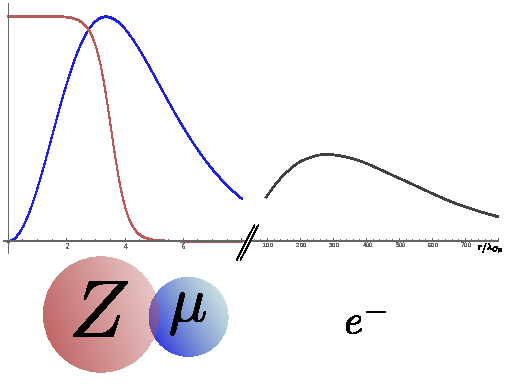
\includegraphics[width=0.75\linewidth]{pics/muon_groundState.pdf}%
\caption{The monopole charge distribution for the nucleus (red) and the $1s_{1/2}$ wave functions of the muon (blue) and the electron (gray, enhanced by a factor of 50) for hydrogen-like uranium. The muonic wave function overlaps strongly with the nuclear charge distribution. Therefore finite nuclear size effects are enhanced in muonic atoms}%
\label{fig:muonGS}%
\end{figure}
%
This means the overlap between muonic wave functions and nucleus is large in this case. Also, a typical energy scale for hydrogen-like systems is the ground state binding energy from Eq.~\eqref{eq:finestructure_formula} for a point-like nucleus, which reads as
\begin{equation}
E_{0,\text{point}}=m_f (1-\sqrt{1-(Z\alpha)^2}),
\end{equation}
and is proportional the fermion mass. As a consequence, for muonic atoms and high charge numbers, muonic transitions can have an energy of several MeV and fine-structure splitting can be on the order of $100\,$keV. Excitation energies of nuclear rotational states are of the same order~\cite{ENSDF} and therefore, an extended nuclear model has to be used, which contains the excited nuclear states of the ground state rotational band. Here, the symmetric rigid rotor model for nuclei with axial symmetry has proved successful in describing heavy muonic atoms, see e.g. Refs.~\cite{tanaka1984,hitlin1970,wu1969,Devons1995}, and also is used in this thesis. The symmetric rigid rotor model is presented in Appendix~\ref{app:rig_rotor}, where also the expressions for the nuclear wave functions in terms of Wigner D-functions can be found. In the symmetric rigid rotor model, the nucleus is described by a charge distribution $\rho(\mathbf{r})$ given in the body fixed nuclear frame, and the Euler angles $\Omega=(\phi,\theta,\psi)$ describe its position in the laboratory frame. The rotational state of the nucleus $\left|IM_IK\right>$ is given by the total nuclear angular momentum quantum number $I$, its projection on the $z$ axis of the laboratory frame $M_I$ and on the $z$ axis of the body fixed frame $K$, where $K$ also corresponds to the ground state angular momentum. As derived in Chapter~\ref{ch:furry_pic}, the muonic bound states without radiative corrections can be obtained by solving the Dirac equation for the nuclear potential. Therefore, the coupled system of muon as a Dirac particle and nucleus as a rigid rotor is described by the eigenvalue equation
\begin{equation}
\text{H} \left(\left|N\right>\otimes \left|\mu\right>\right)= \left(\text{H}_{\text{N}} + \text{H}_\mu + V_{\text{el}}\right) \left(\left|N\right>\otimes \left|\mu\right>\right)= E \left(\left|N\right>\otimes \left|\mu\right>\right),
\label{eq:muon_htotal}
\end{equation}
where $H_{\text{N}}$ is the nuclear rigid rotor Hamiltonian, and ${H_\mu}{=}{\boldsymbol{\alpha} \cdot \mathbf{p} + \beta m_\mu}$ is the free Dirac Hamiltonian for the muon with momentum $\mathbf{p}$, and $\boldsymbol{\alpha}$, $\beta$ are the four Dirac matrices. $\left|N\right>$ is the nuclear state and $\left|\mu\right>$ is the muon state. Following Eq.~\eqref{eq:furry_elPot}, the electric potential energy between muon and nuclear charge distribution reads as
\begin{equation}
\label{eq:muon_elInteract}
V_{\text{el}}(\mathbf{r}_\mu^\prime)=-Z\alpha \int \mathrm{d}^3\mathbf{r}_N^\prime \frac{\rho(\mathbf{r}_N^\prime)}{|\mathbf{r}_\mu^\prime-\mathbf{r}_N^\prime|}.
\end{equation}
It is important to recall, that the nuclear charge distribution is given in the body fixed nuclear frame, thus the integration in Eq.~\eqref{eq:muon_elInteract} in most conveniently performed in this frame. The resulting expression in dependence of the position of the muon, however, is needed in the laboratory frame. Therefore, in the following, a multipole expansion of Eq.~\eqref{eq:muon_elInteract} is performed, and the result is given as a function of the muon position in the laboratory frame and the Euler angles describing the orientation of the nuclear frame. Here, vectors are written in spherical components as $\mathbf{r}_i = (r_i,\vartheta_i,\varphi_i)$ in the laboratory frame and as $\mathbf{r}_i^\prime = (r_i^\prime,\vartheta_i^\prime,\varphi_i^\prime)$ in the body-fixed nuclear frame. Since rotations do not change the absolute values, it holds that $r_i^\prime = r_i$.

With the multipole expansion of the Coulomb potential~\cite{jackson1999}
\begin{equation}
\frac{1}{|\mathbf{r}_\mu^{\,\prime}-\mathbf{r}_N^{\,\prime}|}=\sum_{l=0}^\infty \frac{r_<^l}{r_>^{l+1}}\sum_{m=-l}^l  \text{C}^*_{lm}(\vartheta_N^{\prime},\varphi_N^{\prime})\text{C}_{lm}(\vartheta_\mu^\prime,\varphi_\mu^\prime),
\end{equation}
where $r_<:=\min (r_\mu^\prime,r_N^\prime)$, $r_>:=\max (r_\mu^\prime,r_N^\prime)$, the electric potential~\eqref{eq:muon_elInteract} can be written as
\begin{align}
V_{\text{el}}(\mathbf{r}_\mu^{\,\prime})=&\sum_{l,m}-Z\alpha \left[ \int \text{d}^3r^{\prime}_N \frac{r_<^l}{r_>^{l+1}}\text{C}^*_{lm}(\vartheta_N^{\prime},\varphi_N^{\prime})\rho(\mathbf{r}_N^{\,\prime})\right]\text{C}_{lm}(\vartheta_\mu^{\prime},\varphi_\mu^\prime),
\end{align}
where ${\text{C}_{lm}(\vartheta,\varphi)}{=}{\sqrt{4\pi/(2l+1)}\text{Y}_{lm}(\vartheta,\varphi)}$ are the normalized spherical harmonics.
For axially symmetric charge distributions, only the ${m}{=}{0}$-terms contribute after integrating over the charge distribution. The dependency on the muonic angular variables can be transformed to the laboratory system using the Euler angles by
\begin{equation}
\text{P}_{l}(\cos\vartheta_\mu^\prime)=
 \sum_{m=-l}^l C^*_{lm}(\theta,\phi)C_{lm}(\vartheta_\mu,\varphi_\mu),
\end{equation}
which is a special case of Eq.~\eqref{eq:rot_sphHarm}.
Thereby, the potential as a function of the Euler angles and the muon's position in the laboratory frame reads
\begin{align}
V_{\text{el}}(\mathbf{r}_\mu,\phi,\theta)=&\sum_{l=0}^\infty-Z\alpha \left[ \int \text{d}^3\mathbf{r}^{\prime}_N \frac{r_<^l}{r_>^{l+1}}\text{P}_{l}(\cos \vartheta_N^{\prime})\rho(\mathbf{r}_N^{\,\prime})\right]\sum_{m=-l}^l \text{C}^*_{lm}(\theta,\phi)\text{C}_{lm}(\vartheta_\mu,\varphi_\mu).\notag\\
\eqqcolon &\sum_{l=0}^\infty Q_{\text{el}}^{(l)}(r_\mu)\sum_{m=-l}^lC^*_{lm}(\theta,\phi)C_{lm}(\vartheta_\mu,\varphi_\mu)&\notag\\
\eqqcolon& \sum_{l=0}^\infty V^{(l)}_{\text{el}}(\mathbf{r}_\mu,\phi,\theta),
\label{eq:defmulti}
\end{align}
where $Q_{\text{el}}^{(l)}(r_\mu)$ describe the radial distribution of the multipole moments and the dependency on the muonic angles and the Euler angles is in form of a scalar product of spherical tensor operators. This means that the interaction energy only depends on the relative orientation of the muon with respect to the body fixed nuclear $z^\prime$~axis.

Most nuclei turn out to be symmetric with respect to reflection in the $(x^\prime ,y^\prime)$-plane~\cite{zickendraht1991}. This results in only even-$l$ terms in Eq.~\eqref{eq:defmulti} being non-zero, thus the first two terms are the monopole term $l=0$ and the quadrupole term $l=2$. The next term would be the $l=4$ hexadecapole terms. However, the higher order terms are usually not needed for the correct description of the hyperfine level structure~\cite{BorieRinker1982}. From Eq.~\eqref{eq:defmulti}, it follows that the monopole terms only depends on the muonic radial variable, since it can be written as
\begin{equation}
V_{\text{el}}^{(0)}(r_\mu)=-Z\alpha \int\text{d}^3\mathbf{r}_N^\prime \frac{\rho(\mathbf{r}_N^\prime)}{r_>}.
\end{equation}
In fact, the $l=0$ term is the averaged nuclear potential already derived in Eq.~\eqref{eq:gfac_monopole} in the previous chapter on the $g$ factor of spinless nuclei. As a consequence, the $l=0$-term can be used as a potential in the spherically symmetric Dirac equation to define the unperturbed muonic states as
\begin{equation}
\label{eq:muonicEn}
\left(\boldsymbol{\alpha} \cdot \mathbf{p} + \beta m_\mu + V_{\text{el}}^{(0)}(r_\mu) \right) \left|n\kappa m\right> = E_{n\kappa}\left|n\kappa m\right>.
\end{equation}
The unperturbed nuclear states are the rigid rotor states from Eq.~\eqref{app:rigidRot_state} with
\begin{equation}
\label{eq:nuclEn}
\text{H}_N \left|IM_IK\right> = E_N \left|IM_IK\right>,
\end{equation}
where the excitation energies of the nuclear rotational states are typically taken from experiments~\cite{ENSDF}, and not parametrized by the moment of inertia from Eq.~\eqref{eq:rig_rotorEn}.
The $l=2$ quadrupole term couples nuclear and muonic degrees of freedom and is treated in Section~\ref{sec:muon_dynamic}, and~\ref{sec:muon_residualSO}. The multipole interaction from Eq.~\eqref{eq:defmulti} in general, and the quadrupole interaction with $l=2$ in particular has the structure of a scalar product of two irreducible tensor operators, as defined in Eq.~\eqref{app:tensor_scalarProd}. One operator acts on the nuclear angular variables, i.e. the Euler angles, and one on the muonic angular variables.
For these types of operators, the calculation of expectation values can be simplified by using the theory of irreducible tensor operators, as described in Appendix~\ref{app:ang_theo}. Therefore, states of defined total angular momentum have to be considered as
\begin{equation}
\label{eq:totalState}
\left| FM_F\,IK\,n\kappa\right> = \sum_{M_I, m}\text{C}^{FM_F}_{IM_I\,j(\kappa)m}\left|IM_IK\right>\,\left|n\kappa m\right>
\end{equation}
with total angular momentum $F$, nuclear angular momentum $I$ and muonic angular momentum $j$. The muonic angular momentum $j$ is already composed out of the orbital angular momentum $l$ and the spin angular momentum, as described in Eq.~\eqref{eq:ansatz_dirac}. The total energy of the muon-nucleus system can be calculated as the sum of nuclear energy $E_N$ from Eq.~\eqref{eq:nuclEn}, the muonic energy from Eq.~\eqref{eq:muonicEn} and the expactation value of the quadrupole interaction $\left<V_{\text{el}}^{(2)}\right>$ from Eq.~\eqref{eq:defmulti}.

\subsection{Fine structure of heavy muonic atoms}
\label{sec:muon_finestructure}
In this subsection, the solution of the Dirac equation for the muon will be discussed. In particular, the effects of vacuum polarization in Uehling approximation, recoil corrections, and electron screening are implemented, using known methods. Especially, the usage of the dual-kinetic-balance method~\cite{Shabaev2004} in the framework of muonic atoms is presented. Results are presented for muonic $^{205}$Bi, $^{147}$Sm, and $^{89}$Zr. This subsection follows Ref.~\cite{michel2017}, which was published in the framework of this thesis. 

\subsubsection{Finite nuclear size corrections}
\label{sec:radialEq}
%The total Hamiltonian for a muon bound to a nucleus can be written as a sum of nuclear, muonic, and interaction Hamiltonian~\cite{Devons1995}. Thus, we consider the Hamiltonian
%\begin{equation}
%H = H_{N} + H^{(0)}_{\mu} + H_{\mu - N},
%\end{equation}
%with the nuclear Hamiltonian $H_{N}$, the Dirac Hamiltonian $H^{(0)}_{\mu}$ for the free muon, and the interaction Hamiltonian $H_{\mu - N}$. The nucleus is described in the rotational model, i.e. in a state with well defined angular momentum and charge- and current density in the body fixed nuclear frame~\cite{kozhedub2008}. As a next step, the interaction between the bound muon and the atomic nucleus is expanded, where electric and magnetic interactions are taken into account. The interaction Hamiltonian is
%\begin{equation}
%\label{eq:Hint}
%H_{\mu - N} = H_{E} + H_{M}
%\end{equation}
%where the electric part reads
%\begin{equation}
%\label{eq:elInt}
%H_{E}= - \alpha \int \mathrm{d}V^{\prime}\, \frac{\rho (\mathbf{r}^{\,\prime})}{|\mathbf{r}_{\mu}-\mathbf{r}^{\,\prime}|} ,
%\end{equation}
%with the fine structure constant $\alpha$, the position $\mathbf{r}^{\,\prime}$ of the nuclear charge distribution and the position $\mathbf{r}_{\mu}^{\,\prime}$ of the muon in the nuclear frame. The nuclear charge distribution $\rho(\mathbf{r})$ is normalized to the nuclear charge $Z$ as
%\begin{equation}
%\label{eq:norm}
%\int \mathrm{d}V\rho(\mathbf{r}) = Z.
%\end{equation}
For considering monopole and quadrupole interactions, the nuclear charge distribution is divided into a spherically symmetric part $\rho_0(r)$ and a part $\rho_2(r)$ describing the quadrupole distribution in the nuclear frame as~\cite{hitlin1970}
\begin{equation}
\label{eq:rho}
\rho(\mathbf{r}^{\,\prime}) = \rho_0(r^{\prime}) + \rho_2(r^{\prime}) \, Y_{20}(\vartheta^\prime,\varphi^\prime),
\end{equation}
with the spherical harmonics $Y_{lm}(\vartheta,\varphi)$. Since an analogous part for the dipole distribution would be an operator of odd parity, it would vanish after averaging with muon wave functions of defined parity~\cite{johnson2007}, and thus it is not considered here and neither are higher multipoles beyond the quadrupole term. Correspondingly, the electric potential from Eq.~\eqref{eq:defmulti} contains only the monopole and quadrupole part, and can be written as
\begin{equation}
\label{eq:quadInt}
V_{\text{el}}(\mathbf{r}_\mu,\phi,\theta) = V^{(0)}_{\text{el}}(r_\mu) + V^{(2)}_{\text{el}}(\mathbf{r}_\mu,\phi,\theta),
\end{equation}
where the spherically symmetric part of the charge distribution can be written as
\begin{equation}
\label{eq:Hmonopole}
V^{(0)}_{\text{el}}(r_\mu)= - 4 \pi Z\alpha \int_0^\infty \mathrm{d}r \, r^2 \frac{\rho_0(r)}{r_>},
\end{equation}
with $r_>=\text{max}(r,r_\mu)$. This interaction potential will be included in the numerical solution of the Dirac equation for the muon as described in Section~\ref{sec:radialEq}. The quadrupole part of the interaction $V^{(2)}_{\text{el}}$ causes hyperfine splitting, which is calculated in Section~\ref{sec:muon_dynamic}.\\

The appropriate states have well-defined angular momentum, as introduced in Eq.~\eqref{eq:totalState}. As a basis for further calculations, the Dirac equation
\begin{equation}
\label{eq:diracSph}
\left( \boldsymbol{\alpha}\cdot \mathbf{p}+ \beta + V_{\text{el}}^{(0)}(r_\mu) \right) \ket{n \kappa m} = (1-E^{(B)}_{n \kappa}) \ket{n \kappa m}
\end{equation}
is solved for the muon. Here, $E^{(B)}_{n \kappa}$ are the binding energies, and the potential $V_{\text{el}}^{(0)}(r_\mu)$ is the spherically symmetric part of the interaction with the nucleus. This is the monopole contribution from the electric interaction in Eq.~\eqref{eq:Hmonopole} and, if vacuum polarization is considered, the Uehling potential from Eq.~\eqref{eq:uehl_2}. A Fermi type charge distribution~\cite{Beier2000} is used to model the monopole charge distribution as
\begin{equation}
\label{eq:fermi}
\rho_0 (r)=N\left[1+\text{exp}\left(\cfrac{r-c}{a}\right)\right]^{-1},
\end{equation}
where $a$ is a skin thickness parameter and $c$ the half-density radius. The normalization constant $N$ is chosen such that the volume integral is equal to one, since the charge is already included in the fine-structure constant. It has been proven, that $a=t/(4\,\text{log}3)$, with $t=2.30\,\text{fm}$, is a good approximation for most of the nuclei~\cite{Beier2000}. The parameter $c$ is then determined by demanding, that the charge radius squared
\begin{equation}
\left<r^2\right>=\cfrac{\int\text{d}r \, r^4\rho_0(r)}{\int\text{d}r \, r^2\rho_0(r)}
\end{equation}
agrees with the values from the literature~\cite{Angeli2013}. Since the potential in Eq.~\eqref{eq:diracSph} is spherically symmetric, the angular part can be separated and the solution can be written in terms of the spherical spinors $\Omega_{\kappa m}(\vartheta,\varphi)$ from Eqs.~\eqref{eq:sph_spinor}, \eqref{eq:ansatz_dirac} as~\cite{greiner2000}
\begin{equation}
\ket{n\kappa m}=\frac{1}{r}\colvec{2}{G_{n\kappa}(r)\,\Omega_{\kappa m}}{i\,F_{n\kappa}(r)\,\Omega_{-\kappa m}}.
\end{equation}
The remaining equations for the radial functions are solved with the dual-kinetic-balance method~\cite{Shabaev2004} to obtain $G_{n\kappa}$ and $F_{n\kappa}$, and the corresponding eigenenergies $E_{n\kappa}$ numerically.

In Table~\ref{tab:sphDirac}, the binding energies for muonic $^{205}_{83}$Bi, $^{147}_{62}$Sm, and $^{89}_{40}$Zr are shown, where the finite nuclear size effect is illustrated by also including the binding energies $E^{(C)}_{n\kappa}$ from Eq.~\eqref{eq:finestructure_formula} of the pure Coulomb potential $-Z\alpha / r_\mu$, which read~\cite{greiner2000}
\begin{equation}
\label{eq:finestructure_formula_2}
E^{(C)}_{n\kappa}=1-\left(1+\frac{(Z\alpha)^2}{\left( n-|\kappa|+\sqrt{\kappa^2-(Z\alpha)^2} \right)^2}\right)^{-\frac{1}{2}}.
\end{equation}
Furthermore, the corrections from the Uehling potential in Eq.~\eqref{eq:uehl_2} are shown separately.
The uncertainties include the error in the tabulated RMS radius value as well as a model error, which is estimated via the difference of the binding energies with the Fermi potential from Eq.~\eqref{eq:fermi} and the potential of a charged sphere with the same RMS radius. For heavy nuclei, the finite nuclear size correction can amount up to 50$\,\%$, and thus the binding energy is halved.

%begin table
\begin{table}[b]
\setlength\extrarowheight{3pt}
\caption{\label{tab:sphDirac}
Overview of the binding energies for muonic $^{205}_{83}$Bi, $^{147}_{62}$Sm, and $^{89}_{40}$Zr, obtained by solving the Dirac equation with the spherically symmetric parts of the muon-nucleus interaction.
$E_{\rm{C}}$ are the binding energies \eqref{eq:finestructure_formula_2} for a  point-like nucleus.
$E_{\rm{fs}}$, $E_{\rm{uehl}}$ are the binding energies in the finite-size potential with and without the Uehling correction, respectively.
The reduced mass is used to include the non-relativistic recoil corrections from Section~\ref{sec:recoil}. If not indicated, the uncertainties are negligible. 
All energies are in keV.}
%\begin{ruledtabular}
\centering
\begin{tabular}{c|clll}
& state & $E_{\rm{C}}$& $E_{\rm{fs}}$ &$E_{\rm{uehl}}$\\ \hline \\[-7pt]
$^{205}_{\phantom{1}83}$Bi & $1s_{1/2}$&\text{21573.3} & \text{10699.(51.)} &\text{10767.(52.)} \\
  & $2s_{1/2}$& \text{\phantom{1}5538.6} & \text{\phantom{1}3654.(15.)} & \text{\phantom{1}3674.(15.)}\\
  & $2p_{1/2}$ & \text{\phantom{1}5538.6} & \text{\phantom{1}4893.(3.)} & \text{\phantom{1}4927.(3.)} \\
  & $2p_{3/2}$ & \text{\phantom{1}4958.9} & \text{\phantom{1}4706.(5.)} & \text{\phantom{1}4737.(5.)} \\
  & $3s_{1/2}$ & \text{\phantom{1}2394.3} & \text{\phantom{1}1796.(5.)} & \text{\phantom{1}1804.(6.)} \\
  & $3p_{1/2}$ & \text{\phantom{1}2394.3} & \text{\phantom{1}2170.0(5)} & \text{\phantom{1}2190.1(5)} \\
  & $3p_{3/2}$ & \text{\phantom{1}2221.4} & \text{\phantom{1}2131.(1.)} & \text{\phantom{1}2141.(1.)} \\
  & $3d_{3/2}$ & \text{\phantom{1}2221.4} & \text{\phantom{1}2216.9(3)}& \text{\phantom{1}2227.8(3)}\\
  & $3d_{5/2}$ & \text{\phantom{1}2174.6} & \text{\phantom{1}2172.8(2)} & \text{\phantom{1}2183.0(2)} \\[7pt]
 $^{147}_{\phantom{1}62}$Sm & $1s_{1/2}$& \text{11423.8} & \text{\phantom{1}7165.(28.)} & \text{\phantom{1}7213.(29.)} \\
  & $2s_{1/2}$& \text{\phantom{1}2895.7} & \text{\phantom{1}2230.(7.)} & \text{\phantom{1}2242.(7.)} \\
  & $2p_{1/2}$ & \text{\phantom{1}2895.7} & \text{\phantom{1}2778.(2.)} & \text{\phantom{1}2795.(2.)} \\
  & $2p_{3/2}$ & \text{\phantom{1}2736.9} & \text{\phantom{1}2689.(2.)} & \text{\phantom{1}2706.(2.)} \\
  & $3s_{1/2}$ & \text{\phantom{1}1268.9} & \text{\phantom{1}1061.(2.)} & \text{\phantom{1}1066.(2.)} \\
  & $3p_{1/2}$ & \text{\phantom{1}1268.9} & \text{\phantom{1}1228.6(4)} & \text{\phantom{1}1234.2(4)} \\
  & $3p_{3/2}$ & \text{\phantom{1}1221.7} & \text{\phantom{1}1204.7(6)} & \text{\phantom{1}1210.0(6)} \\
  & $3d_{3/2}$ & \text{\phantom{1}1221.7} & \text{\phantom{1}1221.4(1)} & \text{\phantom{1}1226.2(1)} \\
  & $3d_{5/2}$ & \text{\phantom{1}1207.6} & \text{\phantom{1}1207.4} & \text{\phantom{1}1212.1} \\[7pt]
 $^{89}_{40}$Zr & $1s_{1/2}$& \text{\phantom{1}4595.5} & \text{\phantom{1}3643.(8.)} & \text{\phantom{1}3669.(8.)} \\
  & $2s_{1/2}$& \text{\phantom{1}1155.2} & \text{\phantom{1}1021.(2.)} & \text{\phantom{1}1026.(2.)} \\
  & $2p_{1/2}$ & \text{\phantom{1}1155.2} & \text{\phantom{1}1147.8(2)} & \text{\phantom{1}1153.7(2)} \\
  & $2p_{3/2}$ & \text{\phantom{1}1129.9} & \text{\phantom{1}1127.0(2)} & \text{\phantom{1}1132.6(2)} \\
  & $3s_{1/2}$ & \text{\phantom{11}510.6} & \text{\phantom{11}469.8(5)} & \text{\phantom{11}471.4(5)} \\
  & $3p_{1/2}$ & \text{\phantom{11}510.6} & \text{\phantom{11}508.0(1)} & \text{\phantom{11}509.8(1)} \\
  & $3p_{3/2}$ & \text{\phantom{11}503.1} & \text{\phantom{11}502.0(1)} & \text{\phantom{11}503.8(1)} \\
  & $3d_{3/2}$ & \text{\phantom{11}503.1} & \text{\phantom{11}503.1} & \text{\phantom{11}504.5} \\
  & $3d_{5/2}$ & \text{\phantom{11}500.7} & \text{\phantom{11}500.7} & \text{\phantom{11}502.1} \\

\end{tabular}
%\end{ruledtabular}
\footnotetext[1]{$V(r_\mu)=H^{(0)}_E(r_\mu)$}
\footnotetext[2]{$V(r_\mu)=H^{(0)}_E(r_\mu)+V_{\text{Uehl}}(r_\mu)$
%\footnotetext[3]{$V(r_\mu)=-Z\alpha/r_\mu$
\\see Eq.~\eqref{eq:Hmonopole}, \eqref{eq:diracSph}, and \eqref{eq:uehl_2} for definitions}
\end{table}
%end table
%
%
\subsubsection{Vacuum polarization in Uehling approximation}
\label{sec:qed}

For atomic electrons, there are two QED corrections of the order $\alpha$, namely the self-energy (SE) QED and the vacuum polarization (VP) correction~\cite{Beier2000}, which usually contribute equally. For muons, however, the VP correction is much larger due to virtual electron-positron pairs, which are less suppressed due to the small electron-to-muon mass ratio~\cite{BorieRinker1982}. The spherically symmetric part of the vacuum polarization to first order in $\alpha$ and $Z\alpha$ is the Uehling potential~\cite{Elizarov2005}
\begin{alignat}{2}
&V_{\text{Uehl}}(r_\mu)&&=-\alpha \frac{2\alpha}{3\pi}\int_0^\infty \text{d}r^{\prime}\,4\pi \rho_0(r^\prime)\int_1^\infty \text{d}t\,\left( 1+\frac{1}{2t^2} \right)\nonumber\\[7.5pt]
&&&\times\frac{\sqrt{t^2-1}}{t^2} \frac{\text{exp}(-2m_e|r_\mu-r^\prime|t)-\text{exp}(-2m_e(r_\mu+r^\prime)t)}{4m_er_\mu t},
\label{eq:uehl_2}
\end{alignat}
where $m_e$ is the electron mass and $\rho_0$ is the spherically symmetric part of the charge distribution from Eq.~\eqref{eq:rho}. This potential can be directly added to the Dirac equation~\eqref{eq:diracSph}. In this way, all iterations of the Uehling potential are included~\cite{indelicato2013}. Results for our calculations can be found in Table~\ref{tab:sphDirac}.
%
%
\subsubsection{Recoil corrections}
\label{sec:recoil}
Taking into account the finite mass and the resulting motion of the nucleus leads to recoil corrections to the bound muon energy levels. In nonrelativistic quantum mechanics, as in classical mechanics, the problem of describing two interacting particles can be reduced to a one particle problem by using the reduced mass $m_r$ of the muon-nucleus system~\cite{landaulifshitz3}. With the mass of the nucleus $m_N$, the reduced mass reads in the chosen system of units as
\begin{equation}
\label{eq:redmass}
m_r=\frac{m_N}{m_N+1},
\end{equation}
and the Dirac equation is accordingly modified to
\begin{equation}
\label{eq:diracSphRed}
\left( \boldsymbol{\alpha}\cdot \mathbf{p}+ \beta\,m_r + V_{\text{el}}^{(0)}(r_\mu) \right) \ket{n \kappa m} = (m_r-E^{(B)}_{n \kappa}) \ket{n \kappa m}.
\end{equation}
In relativistic quantum mechanics, this separation is not possible. We follow an approach used in Refs.~\cite{friar1973,BorieRinker1982}, which includes the nonrelativistic part of the recoil correction already in the wave functions by using the reduced mass in the Dirac equation and calculating the leading relativistic corrections perturbatively. If $E^{\text{(fm)}}_{n\kappa}$ denotes the binding energy of Eq.~\eqref{eq:diracSph} with the finite size potential from Eq.~\eqref{eq:Hmonopole}, but with the reduced mass replaced by the full muon rest mass, and $E^{\text{(rm)}}_{n\kappa}$ the binding energy in the same potential but with the reduced mass from Eq.~\eqref{eq:redmass}, then the leading relativistic recoil correction $\Delta E^{\text{(rec,rel)}}_{n\kappa}$ according to Ref.~\cite{BorieRinker1982} reads
\begin{equation}
\label{eq:relrec}
\Delta E^{\text{(rec,rel)}}_{n\kappa} = -\frac{\left(E^{\text{(fm)}}_{n\kappa}\right)^2}{2 M_N}+\frac{1}{2 M_N}\left< h(r) + 2 E^{\text{(fm)}}_{n\kappa} P_1(r)  \right>,
\end{equation}
where $M_N$ is the mass of the nucleus, and the functions $h(r)$ and $P_1(r)$ are defined in Eqs. (109) and (111) of Ref.~\cite{BorieRinker1982}, respectively. In Table~\ref{tab:recoil}, the binding energies obtained by solving the Dirac equation with the muon rest mass and the reduced mass of the muon-nucleus system are compared. Furthermore, the leading relativistic recoil correction is shown. The uncertainties include errors in the RMS radius, the model of the charge distribution and for the relativistic recoil, and a $(m_\mu/M_N)^2$ term due to higher-order corrections in the mass ratio of muon and nucleus, which dominates the uncertainty for lower $Z$.
%begin table
\begin{table}
\setlength\extrarowheight{3pt}
\caption{\label{tab:recoil}Relativistic recoil corrections to the binding energies for muonic $^{205}_{83}$Bi, $^{147}_{62}$Sm, and $^{89}_{40}$Zr. fm (full mass) denotes the finite size binding energy, analogous to the fourth column of Table~\ref{tab:sphDirac}, but with the rest mass of the muon used in the Dirac equation. $\Delta E_{\text{rec,nr}}$ is the non-relativistic recoil correction, which is the difference between the finite size Dirac solutions with reduced mass and full mass, respectively. $\Delta E^{\text{(rec,rel)}}_{n\kappa}$ is the leading relativistic recoil correction from Section~\ref{sec:recoil}. 
If not indicated, the uncertainties are negligible. 
All energies are in keV.}
%\begin{ruledtabular}
\centering
\begin{minipage}{\textwidth}
\centering
\renewcommand*{\thefootnote}{\alph{footnote}}
\begin{tabular}{l|llll}
& state & $E^{\text{(fm)}}$ &$\Delta E^{\text{rec,nr}}$&$\Delta E^{\text{(rec,rel)}}_{n\kappa}$\footnotemark[1]\\ \hline \\[-7pt]
 $^{205}_{\phantom{1}83}$Bi & $1s_{1/2}$& \text{10702.(51.)} & \text{-2.80(4)} & \text{0.39(4)} \\
  & $2s_{1/2}$& \text{\phantom{1}3656.(15.)} & \text{-1.42(2)} & \text{0.09(3)}\\
  & $2p_{1/2}$ & \text{\phantom{1}4895.6(3.0)} & \text{-2.24(1)} & \text{0.12(3)} \\
  & $2p_{3/2}$ & \text{\phantom{1}4708.2(4.6)} & \text{-2.27(1)} & \text{0.01(1)} \\
  & $3s_{1/2}$ & \text{\phantom{1}1796.6(5.5)} & \text{-0.78(1)} & \text{0.03(3)} \\
  & $3p_{1/2}$ & \text{\phantom{1}2180.0(0.5)} & \text{-1.05} & \text{0.03(3)} \\
  & $3p_{3/2}$ & \text{\phantom{1}2131.9(1.3)} & \text{-1.06} & \text{0.03(3)} \\
  & $3d_{3/2}$ & \text{\phantom{1}2218.1(0.3)} & \text{-1.21} & \text{0.02(2)} \\
  & $3d_{5/2}$ & \text{\phantom{1}2174.0(0.2)} & \text{-1.19} & \text{0.02(2)} \\[7pt]
 $^{147}_{\phantom{1}62}$Sm & $1s_{1/2}$& \text{\phantom{1}7168.(28.)} & \text{-3.17(4)} & \text{0.29(7)} \\
  & $2s_{1/2}$& \text{\phantom{1}2231.1(6.7)} & \text{-1.31(1)} & \text{0.05(5)} \\
  & $2p_{1/2}$ & \text{\phantom{1}2779.4(1.5)} & \text{-1.97(1)} & \text{0.05(5)} \\
  & $2p_{3/2}$ & \text{\phantom{1}2691.2(1.8)} & \text{-1.96(1)} & \text{0.04(4)} \\
  & $3s_{1/2}$ & \text{\phantom{1}1062.0(2.3)} & \text{-0.68(1)} & \text{0.02(2)} \\
  & $3p_{1/2}$ & \text{\phantom{1}1229.5(0.4)} & \text{-0.89} & \text{0.01(1)} \\
  & $3p_{3/2}$ & \text{\phantom{1}1205.6(0.6)} & \text{-0.89} & \text{0.01(1)} \\
  & $3d_{3/2}$ & \text{\phantom{1}1222.3(0.1)} & \text{-0.93} & \text{0.01(1)} \\
  & $3d_{5/2}$ & \text{\phantom{1}1208.3} & \text{-0.92} & \text{0.01(1)} \\[7pt]
 $^{89}_{40}$Zr & $1s_{1/2}$& \text{\phantom{1}3646.5(8.2)} & \text{-3.36(3)} & \text{0.15(15)} \\
  & $2s_{1/2}$& \text{\phantom{1}1022.4(1.5)} & \text{-1.11(1)} & \text{0.02(2)} \\
  & $2p_{1/2}$ & \text{\phantom{1}1149.2(0.2)} & \text{-1.43} & \text{0.01(1)} \\
  & $2p_{3/2}$ & \text{\phantom{1}1128.4(0.2)} & \text{-1.41} & \text{0.01(1)} \\
  & $3s_{1/2}$ & \text{\phantom{11}470.3(0.5)} & \text{-0.54} & \text{0.01(1)} \\
  & $3p_{1/2}$ & \text{\phantom{11}508.6(0.1)} & \text{-0.64} & \text{0.00} \\
  & $3p_{3/2}$ & \text{\phantom{11}502.7(0.1)} & \text{-0.63} & \text{0.00} \\
  & $3d_{3/2}$ & \text{\phantom{11}503.7} & \text{-0.64} & \text{0.00} \\
  & $3d_{5/2}$ & \text{\phantom{11}501.3} & \text{-0.63} & \text{0.00} \\
\end{tabular}
%\end{ruledtabular}
\footnotetext[1]{$\Delta E^{\text{rec,nr}}:=E^{\text{(red.mass)}}-E^{\text{(fm)}}$, see Section~\ref{sec:recoil} for definitions.}
\end{minipage}
\end{table}
%end table
%
%
\subsubsection{Interaction with atomic electrons}
\label{sec:screen}
%begin table
\begin{table}
\setlength\extrarowheight{3pt}
\caption{\label{tab:screen}Electron screening corrections $\Delta E_{\rm{S}}$ to the bound muon energy levels for muonic $^{205}_{83}$Bi, $^{147}_{62}$Sm, and $^{89}_{40}$Zr. The subscript '$\rm{eff}$' are the screening corrections with the effective nuclear charge method, whereas '$\rm{3step}$' use the 3 step calculation, both described in Section~\ref{sec:screen}. For the superscript $(1)$, only the 1s electrons are considered, while for $({1}{+}{2})$, all electrons from with $n=1,2$ are considered. All energies are in keV.}
%\begin{ruledtabular}
\centering
\begin{tabular}{c|crrrr}
&$\mu$-state & $\Delta E_{\rm{S,eff}}^{(1)}$  & $\Delta E_{\rm{S,eff}}^{(1+2)}$ & $\Delta E_{\rm{S,3step}}^{(1)}$ & $\Delta E_{\rm{S,3step}}^{(1+2)}$\\ \hline \\[-7pt]
 $^{205}_{\phantom{1}83}$Bi & $1s_{1/2}$& \text{5.555} & \text{10.825} & \text{5.555} & \text{10.825} \\
  & $2s_{1/2}$& \text{5.537} & \text{10.803} & \text{5.538} & \text{10.805} \\
  & $2p_{1/2}$ & \text{5.548} & \text{10.817} & \text{5.549} & \text{10.818} \\
  & $2p_{3/2}$ & \text{5.547} & \text{10.816} & \text{5.548} & \text{10.817} \\
  & $3s_{1/2}$ & \text{5.490} & \text{10.748} & \text{5.494} & \text{10.753} \\
  & $3p_{1/2}$ & \text{5.514} & \text{10.776} & \text{5.516} & \text{10.779} \\
  & $3p_{3/2}$ & \text{5.512} & \text{10.774} & \text{5.515} & \text{10.777} \\
  & $3d_{3/2}$ & \text{5.526} & \text{10.791} & \text{5.528} & \text{10.793} \\
  & $3d_{5/2}$ & \text{5.525} & \text{10.789} & \text{5.527} & \text{10.792} \\[7pt]
 $^{147}_{\phantom{1}62}$Sm & $1s_{1/2}$& \text{3.705} & \text{7.312} & \text{3.705} & \text{7.312} \\
  & $2s_{1/2}$& \text{3.699} & \text{7.305} & \text{3.700} & \text{7.305} \\
  & $2p_{1/2}$ & \text{3.703} & \text{7.309} & \text{3.703} & \text{7.309} \\
  & $2p_{3/2}$ & \text{3.703} & \text{7.309} & \text{3.703} & \text{7.309} \\
  & $3s_{1/2}$ & \text{3.682} & \text{7.285} & \text{3.683} & \text{7.286} \\
  & $3p_{1/2}$ & \text{3.689} & \text{7.293} & \text{3.691} & \text{7.295} \\
  & $3p_{3/2}$ & \text{3.689} & \text{7.293} & \text{3.690} & \text{7.294} \\
  & $3d_{3/2}$ & \text{3.694} & \text{7.299} & \text{3.695} & \text{7.300} \\
  & $3d_{5/2}$ & \text{3.694} & \text{7.298} & \text{3.694} & \text{7.299} \\[7pt]
 $^{89}_{40}$Zr & $1s_{1/2}$& \text{2.214} & \text{4.405} & \text{2.214} & \text{4.405} \\
  & $2s_{1/2}$& \text{2.212} & \text{4.402} & \text{2.212} & \text{4.403} \\
  & $2p_{1/2}$ & \text{2.213} & \text{4.403} & \text{2.213} & \text{4.403} \\
  & $2p_{3/2}$ & \text{2.213} & \text{4.403} & \text{2.213} & \text{4.403} \\
  & $3s_{1/2}$ & \text{2.205} & \text{4.395} & \text{2.206} & \text{4.396} \\
  & $3p_{1/2}$ & \text{2.207} & \text{4.397} & \text{2.208} & \text{4.398} \\
  & $3p_{3/2}$ & \text{2.207} & \text{4.397} & \text{2.208} & \text{4.398} \\
  & $3d_{3/2}$ & \text{2.209} & \text{4.399} & \text{2.210} & \text{4.400} \\
  & $3d_{5/2}$ & \text{2.209} & \text{4.399} & \text{2.209} & \text{4.400} \\

\end{tabular}
%\end{ruledtabular}
\end{table}
%end table
The effect of the surrounding electrons on the binding energies of the muon is commonly referred to as electron screening and was estimated following Ref.~\cite{vogel1973} by calculating an effective screening potential from the charge distribution of the electrons as
\begin{equation}
\label{eq:screenPot}
V_{e}(\mathbf{r}_\mu)=-\alpha \int \mathrm{d}V\frac{\rho_e (\mathbf{r})}{|\mathbf{r}_\mu-\mathbf{r}|},
\end{equation}
and using this potential in the Dirac equation for the muon. The charge distribution of the electrons is obtained by their Dirac wave functions as $\rho_e (\mathbf{r})=\sum_i \psi_{e_i}^*(\mathbf{r})\cdot \psi_{e_i}(\mathbf{r})$, where $\psi_{e_i}(\mathbf{r})$  is the four component spinor of the $i$-th considered electron. In order to obtain the wave functions of the electrons, it has to be taken into account, that the muon essentially screens one unit of charge from the nucleus. The simplest possibility is to replace the nuclear charge by an effective charge $\tilde{Z}=Z-1$ and then solve the Dirac equation for the electron with this modified nuclear potential. Another possibility is to start solving the Dirac equation for the muon in the nuclear potential without electron screening. Then, the Dirac equation for the electron is solved for all required states, with the screening potential due to the bound muon
\begin{equation}
V_{\mu}(\mathbf{r}_e)=-\alpha \int \mathrm{d}V\frac{\psi_\mu^*(\mathbf{r})\cdot \psi_\mu(\mathbf{r})}{|\mathbf{r}_e-\mathbf{r}|},
\end{equation}
analogously to Eq.~\eqref{eq:screenPot}.
The interaction between the electrons is not taken into account here. Finally, the Dirac equation for the muon is solved again, now including the nuclear potential and the screening potential \eqref{eq:screenPot} due the atomic electrons from the considered electron configuration. This procedure can be repeated in the spirit of Hartree's method~\cite{bethe_salpeter} until the electrons and the muon are self-consistent in the fields of each other. Our studies show that one iteration is usually enough since the overlap of muon and electron wave functions in heavy muonic atoms is small. It is important to note, that here the screening potential depends to a small extent on the state of the muon, since the muon wave function is used in the calculation for the electron wave function. The atomic electrons primarily behave like a charged shell around the muon and the nucleus; thus every muon level is mainly shifted by a constant term, which is not observable in muonic transitions. The correction $\Delta E_S$ is defined as the difference of the binding energy without and with screening potential, respectively. Therefore, a positive value indicates that the muon is less bound due to the screening effect. The main contribution to the nonconstant part of the screening potential comes from the 1$s$ electrons, since their wave functions have the biggest overlap with the muon; therefore the exact electron configuration has only a minor effect on transition energies~\cite{vogel1973}. In Table~\ref{tab:screen}, results for the screening correction are shown for both mentioned methods and for different electron configurations. Values of the screening correction for different electron configurations show that a 10\% error for the non-constant part is a reasonable estimate.
%
%
%\section{Hyperfine interactions}
%\label{sec:hfs}
%\subsubsection{Electric quadrupole splitting}
%\label{sec:elQuad1}
%%begin hfs table
%\begin{table*}
%\setlength\extrarowheight{3pt}
%\begin{small}
%\caption{\label{tab:hfs}
%Results for the electric quadrupole and magnetic dipole hyperfine splitting for a selection of hyperfine states of muonic $^{205}_{83}$Bi ($I=\frac{9}{2}$), $^{147}_{62}$Sm ($I=\frac{7}{2}$), and $^{89}_{40}$Zr ($I=\frac{9}{2}$). $\Delta E_Q$ are the values of the electric quadrupole splitting. $\Delta E_M^{\rm{hom}}$ is the magnetic dipole splitting from Eq.~\eqref{eq:hmag} using a homogeneous nuclear current distribution and $\Delta E_M^{\rm{sp}}$ using the nuclear magnetization distribution in the single particle model. See Sections~\ref{sec:elQuad1} and~\ref{sec:magndip} for definitions. All energies are in keV.}
%%\begin{ruledtabular}
%\centering
%\begin{tabular}{c|cllllll}
% nucleus&state&\multicolumn{2}{c}{$\Delta E_Q$}&\multicolumn{2}{c}{$\Delta E_M^{\rm{hom}}$}&\multicolumn{2}{c}{$\Delta E_M^{\rm{sp}}$}\\
% & &$F=I-\frac{1}{2}$&$F=I+\frac{1}{2}$&$F=I-\frac{1}{2}$&$F=I+\frac{1}{2}$&$F=I-\frac{1}{2}$&$F=I+\frac{1}{2}$\\[2pt] \hline \\[-7pt]
%   $^{205}$Bi & $1s_{1/2}$& \phantom{-11}0 & \phantom{-11}0 & -2.27(20) &\phantom{-}1.86(16) & -2.41(20) &\phantom{-}1.97(16) \\
%  & $2s_{1/2}$& \phantom{-11}0 & \phantom{-11}0 & \text{-0.43(5)} &\phantom{-}0.35(4) & -0.47(6) &\phantom{-}0.38(4) \\
%  & $2p_{1/2}$ & \phantom{-11}0 & \phantom{-11}0 & -1.23(11) & \phantom{-}1.01(9) & -1.31(11) &\phantom{-}1.07(10) \\
%  & $2p_{3/2}$ & -175.(24.) & \phantom{-}175.(24.) & -0.55(2) & \phantom{-}0.010(4) & -0.554(22) & \phantom{-}0.098(4) \\
%  & $3s_{1/2}$ & \phantom{-11}0 & \phantom{-11}0 & \text{-0.144(20)} & \phantom{-}0.118(16) & -0.160(20) & \phantom{-}0.131(16) \\
%  & $3p_{1/2}$ & \phantom{-11}0 & \phantom{-11}0 & -0.311(33) & \phantom{-}0.255(26) & -0.336(33) & \phantom{-}0.275(27) \\
%  & $3p_{3/2}$ & \phantom{1}-48.9(8.0) & \phantom{-1}48.9(8.0) & -0.160(7) & \phantom{-}0.028(1) & -0.163(7) & \phantom{-}0.029(1) \\
%  & $3d_{3/2}$ & \phantom{1}-25.4(1.3) & \phantom{-1}25.4(1.3) & -0.161(6) & \phantom{-}0.028(1) & -0.163(6) & \phantom{-}0.029(1) \\
%  & $3d_{5/2}$ & \phantom{-1}28.3(1.3) & \phantom{1}-28.3(1.3) & -0.103(3) & -0.027 & -0.103(3) & -0.027 \\[7pt]
%  $^{147}$Sm & $1s_{1/2}$& \phantom{-11}0 & \phantom{-11}0 & \text{\phantom{-}0.42(18)} & -0.33(14) & \phantom{-}0.25(17) & -0.20(14) \\
%  & $2s_{1/2}$& \phantom{-11}0 & \phantom{-11}0 & \phantom{-}0.072(39) & -0.056(30) & \phantom{-}0.033(39) & -0.026(30) \\
%  & $2p_{1/2}$ & \phantom{-11}0 & \phantom{-11}0 & \phantom{-}0.164(58) & -0.127(45) & \phantom{-}0.106(58) & -0.082(45) \\
%  & $2p_{3/2}$ & \phantom{1}-32.8(3.2) & \phantom{-1}32.8(3.2) & \phantom{-}0.066(8) & -0.004(1) & \phantom{-}0.058(8) & -0.004(1) \\
%  & $3s_{1/2}$ & \phantom{-11}0 & \phantom{-11}0 & \phantom{-}0.023(13) & -0.018(10) & \phantom{-}0.010(13) & -0.008(8) \\
%  & $3p_{1/2}$ & \phantom{-11}0 & \phantom{-11}0 & \phantom{-}0.044(18) & -0.034(14) & \phantom{-}0.026(18) & -0.02(1) \\
%  & $3p_{3/2}$ & \phantom{11}-9.4(1.1) & \phantom{-11}9.4(1.1) & \phantom{-}0.020(3) & -0.001 & \phantom{-}0.017(3) & -0.001 \\
%  & $3d_{3/2}$ & \phantom{11}-3.2(0.1) & \phantom{-11}3.2(0.1) & \phantom{-}0.015(1) & \phantom{-}0.000 & \phantom{-}0.014(1) & \phantom{-}0.000 \\
%  & $3d_{5/2}$ & \phantom{-11}3.7(0.2) & \phantom{11}-3.7(0.2) & \phantom{-}0.010 & \phantom{-}0.004 & \phantom{-}0.010 & \phantom{-}0.004 \\[7pt]
% $^{89}$Zr & $1s_{1/2}$& \phantom{-11}0 & \phantom{-11}0 & \phantom{-}0.36(13) & -0.29(10) & \phantom{-}0.23(12) & -0.19(10) \\
%  & $2s_{1/2}$& \phantom{-11}0 & \phantom{-11}0 & \phantom{-}0.053(23) & -0.043(18) & \phantom{-}0.030(23) & -0.025(18) \\
%  & $2p_{1/2}$ & \phantom{-11}0 & \phantom{-11}0 & \phantom{-}0.071(14) & -0.058(11) & \phantom{-}0.057(14) & -0.047(11) \\
%  & $2p_{3/2}$ & \phantom{-1}12.2(4.7) &\phantom{1}-12.2(4.7) & \phantom{-}0.023(1) & -0.004 & \phantom{-}0.022(1) &-0.004 \\
%  & $3s_{1/2}$ & \phantom{-11}0 & \phantom{-11}0 & \phantom{-}0.016(7) & -0.013(6) & \phantom{-}0.009(7) & -0.007(6) \\
%  & $3p_{1/2}$ & \phantom{-11}0 & \phantom{-11}0 & \phantom{-}0.020(4) & -0.017(4) & \phantom{-}0.016(4) & -0.013(4) \\
%  & $3p_{3/2}$ & \phantom{-11}3.6(1.4) & \phantom{11}-3.6(1.4) & \phantom{-}0.007 & -0.001 & \phantom{-}0.007 & -0.001 \\
%  & $3d_{3/2}$ & \text{\phantom{-11}0.9(0.3)} & \text{\phantom{11}-0.9(0.3)} & \phantom{-}0.004 & \phantom{-}0.000 & \phantom{-}0.004 & \phantom{-}0.000 \\
%  & $3d_{5/2}$ & \text{\phantom{11}-1.1(0.4)} & \text{\phantom{-11}1.1(0.4)} & \phantom{-}0.003 & \phantom{-}0.000 & \phantom{-}0.003 &\phantom{-}0.000 \\
%
%\end{tabular}
%%\end{ruledtabular}
%\end{small}
%\end{table*}
%% end hfs table
%Since for heavy nuclei the nuclear radius is comparable to the muon's Compton wavelength~\cite{Angeli2013,codata}, the muonic wavefunction overlaps strongly with the nucleus and the muon is sensitive to nuclear shape corrections, which results in hyperfine splitting of the energy levels. The quadrupole part of the electric interaction \eqref{eq:quadInt} can be rewritten as~\cite{kozhedub2008}
%\begin{equation}
%\label{eq:Hquad}
%V^{(2)}_{\text{el}}(\mathbf{r}_\mu,\theta,\phi) = - \alpha \frac{Q_0 F_{\text{QD}}(r_\mu)}{2\, r_\mu^3} \sum_{m=-2}^2 C_{2m}(\theta,\phi)C_{2m}^{*}(\vartheta_\mu,\varphi_\mu),
%\end{equation}
%where $C_{lm}(\vartheta,\varphi)=\sqrt{4\pi/(2l+1)}Y_{lm}(\vartheta,\varphi)$ and angles with a subscript $\mu$ describe the position of the muon in the laboratory frame. Here, the nuclear intrinsic quadrupole moment is defined via the charge distribution from Eq.~\eqref{eq:rho} as
%\begin{equation}
%\label{eq:defQ0}
%Q_0 = 2 \sqrt{\frac{4\pi}{5}} \int_0^\infty r^4 \rho_2(r)\,\mathrm{d}r,
%\end{equation}
%and the distribution of the quadrupole moment is described by the function $F_{\text{QD}}(r_\mu)$, with the point-like limit $F_{\text{QD}}(r_\mu)=1$. For the shell model, where the quadrupole distribution is concentrated around the nuclear RMS radius $R_N$, the divergence for $r_\mu=0$ is removed, and the corresponding quadrupole distribution function is
%\begin{equation}
%F_{\text{QD}}(r_\mu)=
%\begin{cases}
%\left(\nicefrac{r_\mu}{R_N}\right)^5 & r_\mu \leq R_N\\
%1 &r_\mu > R_N
%\end{cases}.
%\end{equation}
%Formally, this corresponds to a charge distribution with
%\begin{equation}
%\rho_2(r_\mu)=\frac{Q_0}{2 R_N^4}\sqrt{\frac{5}{4\pi}}\delta(r_\mu-R_N).
%\end{equation}
%The matrix elements of the quadrupole interaction from Eq.~\eqref{eq:Hquad} in the states~\eqref{eq:totalState} read~\cite{Korzinin2005}
%\begin{IEEEeqnarray}{l}
%\label{eq:hquad}
%\bra{FM_FI\kappa}H^{(2)}_E\ket{FM_FI\kappa}= - \alpha (-1)^{j+I+F}
%\left\{\begin{matrix}
%j & I & F\\
%I & j & 2
%\end{matrix}\right\}\\
%\qquad\quad\times \bra{I|}\frac{Q_0}{2} \widehat{C}_2(\vartheta_N,\varphi_N)\ket{|I}
%\bra{n\kappa|}\frac{F_{\text{QD}}(r_\mu)}{r_\mu^{3}}\widehat{C}_2(\vartheta_\mu,\varphi_\mu)\ket{|n\kappa}\nonumber.
%\end{IEEEeqnarray}
%The reduced matrix element in the nuclear coordinates can be expressed with the spectroscopic nuclear quadrupole moment $Q$ as
%\begin{equation}
%\nonumber
%\bra{I|}\frac{Q_0}{2} \widehat{C}_2(\vartheta_N,\varphi_N)\ket{|I}= Q\sqrt{\frac{(2I+3)(2I+1)(I+1)}{4I(2I-1)}},
%\end{equation}
%and the reduced matrix elements in the muonic coordinates are
%\begin{IEEEeqnarray}{l}
%\bra{n\kappa|}f(r_\mu)\widehat{C}_2(\vartheta_\mu,\varphi_\mu)\ket{|n\kappa} =\\[5pt]
%\quad-\sqrt{\frac{(2j+3)(2j+1)(2j-1)}{16j(j+1)}}
%\int_0^\infty \left( G^2_{n\kappa}(r_\mu)+F^2_{n\kappa}(r_\mu)\right)\frac{F_{\text{QD}}(r_\mu)}{r_\mu^{3}} \mathrm{d}r_\mu.\nonumber
%\end{IEEEeqnarray}
%The values for the nuclear RMS radii $R_N$ and the spectroscopic quadrupole moments $Q$ are taken from Refs.~\cite{Angeli2013,Stone2005}. In Table~\ref{tab:hfs}, results for the electric quadrupole hyperfine splitting for the nuclei $^{205}_{83}$Bi, $^{147}_{62}$Sm, and $^{89}_{40}$Zr are shown for a selection of hyperfine states, with uncertainties stemming from the error in the quadrupole moment and an estimation of the modeling uncertainty.
%%
%%
%\subsubsection{Magnetic dipole splitting}
%\label{sec:magndip}
%As for the magnetic part, dipole interaction is considered. Therefore, the corresponding interaction Hamiltonian reads~\cite{Elizarov2005}
%\begin{equation}
%\label{eq:Hmag}
%H_{M} = \frac{|e|}{4 \pi}\,\boldsymbol{\mu}\cdot \left( F_{\text{BW}}(r) \frac{\mathbf{r}}{r^3} \times \boldsymbol{\alpha} \right),
%\end{equation}
%with the charge of the muon $e=-|e|$, the nuclear magnetic moment $\boldsymbol{\mu}$, its distribution function $F_{\text{BW}}$, and the Dirac matrices $\boldsymbol{\alpha}$.
%%If the nuclear current density is described by a normalized scalar function $f_\mu(r)$ as
%%\begin{equation}
%%\label{eq:currentdistr}
%%\mathbf{j}(r)= \text{rot}\left(\boldsymbol{\mu}f_\mu(r)\right),
%%\end{equation}
%%then the distribution function is given by
%%\begin{equation}
%%\label{eq:Fbw}
%%F_{\text{BW}}(r)=-r^2 \frac{\partial}{\partial r}\,\int \text{d}V^{\prime}\,\frac{f_\mu(r^{\prime})}{|\mathbf{r}-\mathbf{r}\,^{\prime}|}.
%%\end{equation}
%The difference in the hyperfine splitting between a point-like magnetic moment and a spatial distribution of the magnetization is called the Bohr-Weisskopf effect~\cite{bohrWeisskopf1950}. In the following, the diagonal matrix elements of the magnetic interaction are analyzed, paying special attention to the distribution function $F_{\text{BW}}$. We expect the contribution of the higher-order terms, namely electric octupole, magnetic quadrupole, and beyond, to be smaller than the uncertainty of the considered terms~\cite{Devons1995,Steffen1985}. Therefore they can be ignored here.
%
%The hyperfine splitting arises from the interaction of the nuclear magnetic moment with the muon's magnetic moment, which is also sensitive to the spatial distribution of the nuclear currents.
%Since the magnetic moment of the muon is inversely proportional to its mass, the magnetic hyperfine splitting in muonic atoms is less important than in electronic atoms. The matrix elements of the corresponding Hamiltonian~\eqref{eq:Hmag} in the state~\eqref{eq:totalState} are~\cite{Korzinin2005}
%\begin{IEEEeqnarray}{l}
%\label{eq:hmag}
%\bra{FM_FI\kappa}H_M\ket{FM_FI\kappa}=
%\,\,\left[ F(F+1)-I(I+1)-j(j+1)\right] \\[7.5pt]
%\qquad\qquad\qquad\qquad\,\,\times\frac{\alpha}{2 m_p}\frac{\mu}{\mu_N}\frac{\kappa}{Ij(j+1)}\int_0^\infty \frac{G_{n\kappa}(r_\mu)F_{n\kappa}(r_\mu)F_{\text{BW}}(r_\mu)}{r_\mu^2}\mathrm{d}r_\mu,\nonumber
%\end{IEEEeqnarray}
%where $m_p$ is the proton mass, and the ratio of the observed magnetic moment $\mu:=\bra{II}(\boldsymbol{\mu})_z\ket{II}$ and the nuclear magneton $\mu_N$ can be found in the literature~\cite{Stone2005}. For the simple model of a homogeneous nuclear current, the distribution function of the Bohr-Weisskopf effect reads
%\begin{equation}
%\label{eq:bwsimple}
%F_{\rm{BW}}(r_\mu)=\begin{cases}
%\left( \nicefrac{r_\mu}{R_N} \right)^3 & r_\mu \leq R_N\\
%1 &r_\mu > R_N
%\end{cases}.
%\end{equation}
%Furthermore, an additional method is used to obtain the distribution function $F_{\rm{BW}}$ from the nuclear single particle model, where the nuclear magnetic moment is assigned to the odd nucleon and the Schrödinger equation for this nucleon is solved in the Woods-Saxon potential of the other nucleons~\cite{Elizarov2005}. In Table~\ref{tab:hfs}, results for the magnetic dipole hyperfine splitting for the nuclei $^{205}_{83}$Bi, $^{147}_{62}$Sm, and $^{89}_{40}$Zr are presented for a selection of hyperfine states, using both methods for obtaining $F_{\rm{BW}}$, where the model error is estimated by the difference of these two methods and the uncertainty in the magnetic moment is also taken into account.
%

\subsection{Dynamical hyperfine structure}
\label{sec:muon_dynamic}
In this subsection, the hyperfine structure of muonic atoms is discussed in detail. In electronic systems, the energy splitting due to hyperfine interactions is usually calculated in first order perturbation theory. This is not enough for the correct prediction of the level structure of heavy muonic atoms.  There are two reasons for this:

Firstly, the fine-structure splitting between states of the same parity, especially between the $2p_{1/2}$ and $2p_{3/2}$ states, is up to the energy scale of a few hundred keV. On the other hand, the first order energy correction due to the electric quadrupole interaction can also be on the order of 100 keV in the $2p_{3/2}$ states. It should be noted that the expectation value of the quadrupole interaction in the $2p_{1/2}$ states vanishes because of angular momentum selection rules. The quadrupole interaction is represented as a rank 2 tensor operator, thus the sum of the involved angular momenta must also be larger than or equal to 2. This is not the case for the expectation value of the $2p_{1/2}$ states with $j=1/2$. There are, however, also the non-diagonal matrix elements with one $2p_{1/2}$ and one $2p_{3/2}$ states, which are also on the hundred keV level for high $Z$ muonic atoms. If the quadrupole hyperfine structure is only calculated in first order perturbation theory, these non-diagonal elements are not considered. Since the separation between the two unperturbed states ($2p_{1/2}$ and $2p_{3/2}$) is on the same level as the non-diagonal matrix elements, first order perturbation theory is not sufficient. As a consequence, the non-diagonal matrix elements have to be taken into account. One possibility would be to use higher order perturbation theory, which involves a sum over the complete muonic spectrum. However, already the consideration of the non-diagonal matrix elements for a muonic fine-structure doublet can explain the majority of the higher order effects. Therefore, the formalism of quasi-degenerate perturbation theory~\cite{sakurai1994} is useful, and the general approach will be briefly reviewed in the following section. Here, the quadrupole interaction is rediagonalized in finite-dimensional subspaces by only using a small number of muonic states.

Secondly, the energy scale of the fine structure and electric quadrupole splitting is on the same scale as the typical excitation energy of the excited nuclear states in the rotational ground state band. In addition, the nuclear states in the ground state rotational band have the same parity and thus are coupled to each other by the quadrupole interaction. This means that the expectation value of the quadrupole operator is generally non-zero, also for the case of different nuclear rotational states. As a consequence, the excited nuclear states have to be taken into account when rediagonalizing the quadrupole interaction in finite-dimensional subspaces as mentioned above.

\subsubsection{Quasi-degenerate perturbation theory}
\label{sec:almostDeg}
In this section, the general approach to quasi-degenerate perturbation theory is briefly reviewed, following~\cite{BorieRinker1982,sakurai1994}, before it will be applied to muonic atoms in the following sections. For simplicity, a system with unperturbed eigenstates $\left|n\right>$ and corresponding unperturbed energies $\mathcal{E}_n$ is investigated. The corresponding eigenvalue equation is
\begin{equation}
H_0 \left|n\right> = \mathcal{E}_n \left|n\right>,
\end{equation}
where $H_0$ is the unperturbed Hamiltonian. Now, a perturbation $H_1$ is considered.
The connection to the muonic atom case can be made by considering $\left|n\right>$ as a multi-index for all the quantum numbers of the muonic atom and using the quadrupole interaction for the perturbation $H_1$. The perturbed eigenvalue equation reads
\begin{equation}
\label{eq:pert_Htot}
\left(H_0 + H_1\right) \left|a\right> = E_a \left|a\right>.
\end{equation}
If $m$ different states $\left| n_i \right>$ are almost degenerate, their energy separation is on the same order as the first order correction due to $H_1$. In this case, the corresponding modelspace is defined as all $\left| n_i \right>$ with $i\in \{1,...,m\}$, if necessary the states have to be relabeled, such that the lowest indices correspond to the states defining the model space.
The projector~$\text{P}$ on the modelspace is defined by acting on an eigenstate $\left|a\right> = \sum_n a_n \left|n\right>$ of Eq.~\eqref{eq:pert_Htot} as
\begin{equation}
\text{P}\left|a\right> = \sum_{i=1}^m a_i \left|n_i\right>,
\end{equation}
thus considering only the states inside of the modelspace.
Analogously, the projector~$\text{Q}$ is defined as the complement, i.e. keeping only coefficients of states outside of the modelspace. Thereby, it holds that $\text{P}+\text{Q}=\rm 1\hspace*{-0.4ex}\rule{0.1ex}{1.52ex}\hspace*{0.2ex}$ and the following relations~\cite{BorieRinker1982} can be derived for eigenstates of the total Hamiltonian from Eq.~\eqref{eq:pert_Htot}:
\begin{alignat}{2}
&\text{Q}\left|a\right> &&= - (H_0-E_a)^{-1}\text{Q}H_1 \left|a\right>,\notag\\
 (H_0-E_a+\text{P}H_1)&\text{P}\left|a\right>&&= -\text{P}H_1\text{Q}\left|a\right>.
\end{alignat}
A combination of these two equations results in
\begin{equation}
\text{P}\left( \,
(H_0-E_a+H_1)\text{P}\left|a\right>
- H_1(H_0-E_a)^{-1}\text{Q}H_1\left|a\right>
\right) = 0,
\label{eq:pert_projectionEq}
\end{equation}
which can be expanded in $\text{Q}$. Thereby, states outside of the finite dimensional modelspace can be treated systematically. The zero-order term is obtained by neglecting the term containing a $\text{Q}$ operator:
\begin{equation}
\label{eq:pert_firstOrder}
\text{P}\left(H_0+H_1-E_a\right) \text{P}\left|a\right> = 0.
\end{equation}
This is essentially Eq.~\eqref{eq:pert_Htot}, but projected on the modelspace. To zeroth order in the projection operator $Q$, the states outside of the modelspace can be neglected. Since this is a finite-dimensional system, an exact solution can be obtained by diagonalization of the Hamiltonian matrix.

When applied to muonic atoms, the unperturbed Hamiltonian is the sum of  a rigid rotor Hamiltonian for the nucleus and Dirac Hamiltonian with the monopole potential for the muon. The perturbation is the hyperfine (mainly quadrupole) interaction. Then, a modelspace needs to be chosen, for example the first few nuclear rotational states and a muonic fine-structure doublet like the ($2p_{1/2}$, $2p_{3/2}$) or ($3d_{3/2}$, $3d_{5/2}$) states. Finally, the diagonal and non-diagonal matrix elements of the hyperfine interactions need to be calculated for all states in the modelspace and the matrix representation of the total Hamiltonian in the modelspace has to be diagonalized.

The solution of Eq.~\eqref{eq:pert_firstOrder} results in an approximation for the eigenstates of the full Hamiltonian as
\begin{equation}
\label{eq:pert_firstOrderState}
\left|a^{(0)}\right> = \sum_{i=1}^m a_i^{(0)}\left|n_i\right>,
\end{equation}
which is a linear combination of the unperturbed states forming the modelspace with the coefficients obtained from the diagonalization of the Hamiltonian matrix. The corresponding eigenvalues are the approximations $E_a^{(0)}$ of the eigenenergy.

Eq.~\eqref{eq:pert_projectionEq} is used for the leading order corrections due to the operator $\text{Q}$, including the Q-dependent term. However, only the effect on the modelspace is investigated, corresponding to the approximation $\left|a\right> \approx \text{P}\left|a\right>$. Using the property of a projection operator $\text{P}^2=\text{P}$, Eq.~\eqref{eq:pert_projectionEq} can be written as
\begin{equation}
\label{eq:pert_secondOrder}
 \underbrace{\text{P}(H_0+H_1-E_a)\text{P}}_{\tilde{H}_0} + \underbrace{\text{P}(H_1(E_a-H_0)^{-1}\text{Q}H_1)\text{P}}_{\tilde{H}_1} \left|a\right> = 0,
\end{equation}
which takes the form of an eigenvalue problem with the unperturbed Hamiltonian $\tilde{H}_0$ and the perturbation $\tilde{H}_1$. Because of $\text{P}$ on the left and right side, this is a finite dimensional problem, although each matrix element of $\tilde{H}_1$ involves a summation over the complete spectrum as shown below. The unperturbed solutions are given by Eq.~\eqref{eq:pert_firstOrderState}. Thereby, the energy correction due to the perturbation $\tilde{H}_1$ can be calculated within first order perturbation theory as
\begin{alignat}{2}
\label{eq:pert_secondOrderEnerg}
&E_a^{(1)}&&= \left<a^{(0)} \middle| \tilde{H}_1 \middle| a^{(0)} \right>\\[7.5pt]
& &&= \sum_{k>m} \frac{\left<a^{(0)}\middle|H_1\middle|n_k\right>\left<n_k\middle|H_1\middle|a^{(0)}\right>}{E_a^{(0)}-\mathcal{E}_{n_k}}\\[7.5pt]
& &&= \sum_{i,j=1}^m a_i^{(0)\,*}a_j^{(0)} \sum_{k>m} \frac{\left<n_i\middle|H_1\middle|n_k\right>\left<n_k\middle|H_1\middle|n_j\right>}{E_a^{(0)}-\mathcal{E}_{n_k}}\notag,
\end{alignat}
where the projector on states outside of the modelspace is formally written as $\text{Q}=\sum_{k>m}\left|n_k\right>\left<n_k\right|$. If there are continuous parts in the spectrum, this sum also involves integrals. Once the zeroth order energies and states are found by diagonalizing the Hamiltionian in the modelspace, the first order energy correction due to states outside of the modelspace is calculated by calculating the second order energy correction due to the original perturbation $H_1$, but the intermediate sum only involves states not contained in the modelspace, i.e. those not already considered in the diagonalization. As a result, the sum $E_a = E_a^{(0)}+E_a^{(1)}$ contains a complete second order treatment of the perturbation $H_1$, and additionally the contributions of the states in the modelspace to all orders.

For actual calculations in the context of muonic atoms, these computations are very time-consuming for the following reasons: Already the unperturbed Hamiltonian involves a numerical solution of the Dirac equation with an extended nuclear monopole potential. The diagonal and non-diagonal matrix elements of the electric quadrupole interaction have to be calculated via numerical integration as well, before diagonalizing the total Hamiltonian. Since finite-basis-set methods~\cite{Shabaev2004} are used in this thesis for solving the Dirac equation, a numerical, discrete representation of the complete muonic spectrum is obtained. Therefore numerical evaluations of Eq.~\eqref{eq:pert_secondOrderEnerg} without approximations is possible in the framework of this thesis.\\

In the following sections, the approach of quasi-degenerate perturbation theory from Section~\ref{sec:almostDeg} will be applied to muonic atoms considering electric monopole and quadru\-pole interaction, as well as magnetic dipole interaction. The starting point is a given deformed nuclear charge distribution $\rho(\mathbf{r})$ and a distribution of the static currents $\mathbf{j}(\mathbf{r})$ inside the nucleus.
The necessary steps are the following:
\begin{itemize}
\item definition of the unperturbed  and perturbed Hamiltonian
\item calculation of the potentials starting from the given charge and current distribution
\item solve the Dirac equation with the electric monopole potential
\item definition of modelspaces
\item calculation of diagonal and non-diagonal matrix elements of the hyperfine operators in the modelspace and rediagonalization
\item calculation of energy correction due to states outside of the modelspace
\end{itemize}


\subsubsection{Non-diagonal elements of hyperfine interactions}
\label{sec:non-diagElements}
The unperturbed Hamiltonian for the muonic atom is already given by Eq.~\eqref{eq:muonicEn} for the nucleus and in Eq.~\eqref{eq:nuclEn} for the muon in terms of the nuclear charge distribution $\rho(\mathbf{r})$. The corresponding states of defined total angular momentum $F$ are given in Eq.~\eqref{eq:totalState}.
The next step for the calculation of the hyperfine structure of muonic atoms in the framework of quasi-degenerate perturbation theory is the computation of the diagonal and non-diagonal matrix elements of the electric quadrupole and magnetic dipole interactions.

The multipole expansion of the electric potential in Eq.~\eqref{eq:defmulti} can be used to express the electric quadrupole interaction energy in terms of the nuclear charge distribution. The quadrupole terms with $l=2$ is
\begin{equation}
V^{(2)}_{\text{el}}(\mathbf{r}_\mu,\phi,\theta)\hspace{-3pt}=\hspace{-3pt}-Z\alpha\hspace{-4pt} \left[ \int \text{d}^3\mathbf{r}^{\prime}_N \frac{\min(r_N,r_\mu)^2}{\max(r_N,r_\mu)^{3}}\text{P}_{2}(\cos \vartheta_N^{\prime})\rho(\mathbf{r}_N^{\,\prime})\right]\hspace{-3pt}\sum_{m=-2}^2 \text{C}^*_{2m}(\theta,\phi)\text{C}_{2m}(\vartheta_\mu,\varphi_\mu).
\label{eq:quadPot}
\end{equation}
As a next step, the matrix element of~\eqref{eq:quadPot} with two arbitrary states from Eq.~\eqref{eq:totalState} is considered, which reads as
\begin{equation}
\Delta E^{(2)}=\left<F_1M_1\,I_1K \,n_1\kappa_1 \middle| V^{(2)}_{\text{el}} \middle|F_2M_2\,I_2K \,n_2\kappa_2 \right>.
\label{eq:quadPotEl}
\end{equation}
With the relation $\text{C}_{lm}^*(\vartheta,\varphi) =(-1)^m\text{C}_{l\,(-m)}(\vartheta,\varphi)$, and fact that the normalized spherical harmonic are irreducible tensor operators as introduced in Appendix~\ref{app:ang_theo}, the sum in Eq.~\eqref{eq:quadPot} is a scalar product of two rank-2 irreducible tensors. Therefore, Eq.~\eqref{app:reducedMatEl_expectation} can be used to rewrite the matrix element from Eq.~\eqref{eq:quadPotEl} in terms of the reduced matrix elements of the spherical harmonics as
\begin{alignat}{2}
&\Delta E^{(2)} =&& -Z\alpha\delta_{F_1F_2}\delta_{M_1M_2} (-1)^{F+I_2+j_1}
\begin{Bmatrix}
I_1 & I_2 & 2 \\
j_2 & j_1&F
\end{Bmatrix}
\left<I_1K\middle|\middle|\text{C}_2 \middle|\middle| I_2 K \right>\\[7.5pt]
&&&\times\left<n_1\kappa_1\middle|\middle|\text{C}_2  \int \text{d}^3\mathbf{r}^{\prime}_N \frac{r_<^2}{r_>^{3}}\text{P}_{2}(\cos \vartheta_N^{\prime})\rho(\mathbf{r}_N^{\,\prime}) \middle|\middle| n_2\kappa_2 \right>,
\label{eq:quadNonDiagEl}
\end{alignat}
where it is useful to define
\begin{equation}
\label{eq:quadDistr}
f_Q(r_\mu)/r_\mu^3 \coloneqq \int \text{d}^3\mathbf{r}^{\prime}_N \frac{r_<^2}{r_>^{3}}\text{P}_{2}(\cos \vartheta_N^{\prime})\rho(\mathbf{r}_N^{\,\prime}),
\end{equation}
since for the approximation of a point-like quadrupole moment or generally for large $r_\mu$ it holds that $f_Q(r_\mu)=1$, and thus the usual $r_\mu^{-3}$ radial integral for quadrupole hyperfine structure is recovered. Accordingly, $f_Q(r_\mu)$ describes the finite distribution of the quadrupole moment inside the nucleus. The reduced matrix element in the nuclear coordinates can be calculated with the rigid rotor wave functions from Appendix~\ref{app:rig_rotor} and the definition of the reduce matrix element from Eq.~\eqref{app:wignerEckardt}. It is given in Eq.~\eqref{eq:rigidRotRedElement} and reads
\begin{equation}
\left< I_1K\middle|\middle|\text{C}_l\middle|\middle|I_2K\right>=(-1)^{I_2+K}
\sqrt{(2I_1+1)(2I_2+1)}
\left(
\begin{matrix}
I_1&I_2&l\\
-K&K&0
\end{matrix}
\right).
\end{equation}
The reduced matrix elements in the muonic variables can be evaluated as~\cite{johnson2007}
\begin{alignat}{2}
&&&\left< n_1\kappa_1\big{|}\big{|}f(r_\mu)\text{C}_l(\vartheta_\mu,\varphi_\mu) \big{|}\big{|}n_2\kappa_2\right> =
 (-1)^{j_1+1/2} \sqrt{(2j_1+1)(2j_2+1)}
\notag\\[7.5pt]
&&&\times
\left(
\begin{matrix}
j_1&j_2&l\\
-\frac{1}{2}&\frac{1}{2}&0
\end{matrix}
\right)\pi(l_1+l_2)\int \text{d}r ({g_{n_1\kappa_1}(r)g_{n_2\kappa_2}(r)}{+}{f_{n_1\kappa_1}(r)f_{n_2\kappa_2}(r)}) f(r_\mu),
\end{alignat}
where $f_{n\kappa}(r_\mu)$ and $g_{n\kappa}(r_\mu)$ are the radial wave functions~\eqref{eq:radial_equations_small} obtained by solving the Dirac equation~\eqref{eq:muonicEn}.
The function
\begin{equation}
\label{eq:parityFunc}
\pi(n) =
\left\{
\begin{matrix}
1\,\text{, {\it n} even;}\phantom{11}\\
0\,\text{, otherwise}
\end{matrix}
\right.
\end{equation}
represents the parity selection rules.
Thus, the evaluation of a single reduced muonic matrix element requires one numerical integration, and for every calculation of $f_Q(r_\mu)$ therein, another numerical integration of Eq.~\eqref{eq:quadDistr} has to be performed.

In the following, the matrix elements of the magnetic hyperfine structure will be calculated for diagonal elements, and for non-diagonal matrix elements in the framework of the rigid rotor nuclear model, following the analysis in Ref.~\cite{Steffen1985}. The magnetic Hamiltonian due to the vector potential $\mathbf{A}_N$ caused by the nuclear static currents in the nuclear body fixed frame reads
\begin{equation}
\label{eq:Hmag_rot}
\text{H}_{M}(\mathbf{r}_\mu) = |e|\,\boldsymbol{\alpha}\cdot \mathbf{A}_N(\mathbf{r}_\mu),
\end{equation}
where the vector potential is generated by the static currents in the nucleus, and the connection reads~\cite{jackson1999}
\begin{equation}
\mathbf{A}_N(\mathbf{r}_\mu) = \frac{1}{4\pi}\int\text{d}^3\mathbf{r}^\prime \frac{\mathbf{j}(\mathbf{r}^\prime)}{|\mathbf{r}_\mu-\mathbf{r}^\prime|}.
\end{equation}
For extended nuclei without a divergence at the origin the current distribution can be expressed in terms of the curl of another vector field, since the divergence of the current distribution in the static case is zero~\cite{jackson1999}. This field is called magnetization $\mathbf{M}(\mathbf{r})$ and the connection between current distribution and magnetization is
\begin{equation}
\mathbf{j}(\mathbf{r}) = \boldsymbol{\nabla} \times  \mathbf{M}(\mathbf{r}).
\end{equation}
The restriction to magnetic dipole interactions is done by writing the magnetization as
\begin{equation}
\mathbf{M}(\mathbf{r})=\boldsymbol{\mu}f(r)=\mu\mathbf{e}_z^\prime\,f(r),
\end{equation}
where $\boldsymbol{\mu}$ is the nuclear magnetic dipole operator and $\mu$ its absolute value. The second equality follows from the fact, that the symmetric rigid rotor model is used and the magnetic moment has to be aligned with the nuclear body fixed $z$-axis $\mathbf{e}_z^\prime$. Otherwise, axial symmetry would be violated.
In Cartesian coordinates in the laboratory system, the basis vector $\mathbf{e}_z^\prime$ of the body fixed system reads as
\begin{equation}
\label{eq:magMomOp}
\boldsymbol{\mu}(\theta,\phi)=|\boldsymbol{\mu}|
\begin{pmatrix}
\sin\theta\cos\phi \\ \sin\theta\sin\phi \\ \cos\theta
\end{pmatrix}.
\end{equation}
The scalar function $f(r)$ describes the finite distribution of the dipole moment in the nucleus, which is responsible for the Bohr-Weisskopf effect~\cite{bohrWeisskopf1950} and is normalized as
\begin{equation}
4\pi\int_0^\infty \text{d}r\,r^2\,f(r)=1.
\end{equation}
Thereby, the magnetic Hamiltonian can be written as
\begin{equation}
\label{eq:hmag_rot2}
\text{H}_M(\mathbf{r}_\mu,\theta,\phi) =\frac{|e|}{4\pi}\boldsymbol{\mu}(\theta,\phi)\cdot
\left( F_{\text{BW}}(r)\frac{\mathbf{r}}{r^3}\times \boldsymbol{\alpha}\right),
\end{equation}
and the function $F_{\text{BW}}(r)$ is connected to the distribution function $f(r)$ via
\begin{equation}
F_{\text{BW}}(r)=-4\pi r^2\partial_r \left(\int_0^\infty\text{d}r^\prime \frac{r^{\prime\,2}f(r^\prime)}{\max (r,r^\prime)}\right).
\end{equation}
The magnetic dipole Hamiltonian from Eq.~\eqref{eq:hmag_rot2} can be written as a scalar product of two rank-1 irreducible tensor operators acting on the muonic and nuclear coordinates, respectively, as~\cite{johnson2007}
\begin{alignat}{2}
&\text{H}_M  (\mathbf{r}_\mu,\theta,\phi) &&=\sum_{\lambda=-1}^1 (-1)^\lambda \;t_\lambda(\mathbf{r}_\mu) \;\;\mu_{-\lambda}(\theta,\phi),\notag\\[7.5pt]
&\qquad \quad t_\lambda(\mathbf{r}_\mu) &&= \frac{-i\sqrt{2}|e|}{4\pi}\left(\boldsymbol{\alpha}\cdot\mathbf{C}^{(0)}_{1\lambda}(\vartheta_\mu,\varphi_\mu)\right)\frac{F_{\text{BW}}(r_\mu)}{r_\mu^2}\,\notag,
\end{alignat}
where $\mathbf{C}^{(a)}_{b\,c}(\vartheta,\varphi)$ are the vector spherical harmonics~\cite[Section 7.]{varshalovich1988} and $\mu_\lambda$ are the spherical components with $\lambda = -1,0,1 $~\cite[Section 1.]{varshalovich1988} of the magnetic moment operator from Eq.~\eqref{eq:magMomOp}. Correspondingly, Eq.~\eqref{app:reducedMatEl_expectation} can be used for the calculation of the expectation value, and the result is
\begin{alignat}{2}
& \left<F_1M_1\,I_1K\,n_1\kappa_1 \middle|\text{H}_M \middle|F_2M_2\,I_2K\,n_2\kappa_2 \right> = \delta_{F_1F_2}\delta_{M_1M_2}(-1)^{F_1+j(\kappa_2)+I_1}\\[7.5pt]
&\qquad\qquad\qquad\times
\begin{Bmatrix}
j(\kappa_1)&j(\kappa_2)&1\\
I_2&I_1&F_1
\end{Bmatrix}
\left< n_1\kappa_1\middle|\middle|t \middle|\middle| n_2\kappa_2\right>
\left< I_1K\middle|\middle|\mu \middle|\middle|I_2K\right>.
\end{alignat}
The reduced matrix elements of the nuclear magnetic moment operator can be obtained with literature values of the magnetic moment  from~\cite{Stone2005} and with Eq.~\eqref{eq:rigidRotRedElement}, using the relation
\begin{equation}
\left< IK\middle|\middle|\mu \middle|\middle|IK\right> =
|\mathbf{\mu}| \left< IK\middle|\middle|C_1 \middle|\middle|IK\right>.
\end{equation}
The reduced muonic matrix elements can be evaluated as~\cite{johnson2007}
\begin{alignat}{2}
\left< n_1\kappa_1\middle|\middle|t \middle|\middle| n_2\kappa_2\right> = -\frac{|e|}{4\pi}(\kappa_1+\kappa_2)(-1)^{j(\kappa_1)+1/2}\sqrt{(2j(\kappa_1)+1)+(2j(\kappa_2)+1)}\qquad\quad\;\\[7.5pt]
\times
\begin{pmatrix}
j(\kappa_1)&j(\kappa_2)&1\\
-1/2&1/2&0
\end{pmatrix}
\pi(l(-\kappa_1)+l(\kappa_2)+1)\int_0^\infty \text{d}r F_{\text{BW}}(r)\left(f_{n_1\kappa_1}g_{n_2\kappa_2}+f_{n_2\kappa_2}g_{n_1\kappa_1} \right).
\end{alignat}

\subsubsection{Rediagonalization of muonic fine-structure doublets}
\label{sec:toyModelRediag}
The concept of rediagonalization in the context of quasi-degenerate perturbation theory was introduced in Section~\ref{sec:almostDeg}. The unperturbed Hamiltonian is introduced in Eqs.~\eqref{eq:muonicEn} and~\eqref{eq:nuclEn} for the unperturbed states from Eq.~\eqref{eq:totalState}. The matrix elements necessary for the rediagonalization of the hyperfine states are discussed in Section~\ref{sec:non-diagElements} for the general case. Thereby, all necessary ingredients for the rediagonalization in the dynamical hyperfine structure of muonic atoms are available. In this section, this concept is applied to a simplified part of the muonic $^{185}$Re spectrum for clarification. The $^{185}$Re nucleus has a ground state angular momentum of $I=5/2$~\cite{Stone2005}, and in this section, the first two excited nuclear states with angular momentum quantum numbers of $7/2$ and $9/2$ are considered. As for the muonic states, the ($2p_{1/2}$,$2p_{3/2}$) fine-structure doublet is considered. 
As a first step, it has to be considered, which unperturbed states $\left|FM_F\,IK\,n\kappa\right>$ can be formed by the nuclear and the muonic states. In general, for every possible value of $F$, the projection quantum number has $(2F+1)$ possible values: $M_F\in \{-F,...,F\}$. The minimal value for $F$ is $F_{\text{min}}=\min(|j(\kappa)-I|)_{\kappa, I}$ and the maximal value for $F$ is $F_{\text{max}}=\max(j(\kappa)+I)_{\kappa, I}$ for the considered values of $\kappa$ and $I$. In this example, the values are $F_{\text{max}}=6$ and $F_{\text{min}}=1$. As a next step, it has to be checked for every value of $F$, which combinations of muonic and nuclear states of the modelspace are able to have the $F$ value. For this, the triangle equation $|j(\kappa)-I|\leq F \leq j(\kappa)+I$ has to hold. In this way, a modelspace is separated into distinct blocks, each with a value of $F$ and a corresponding subset of states from the modelspace, which can form this $F$ value. Since the hyperfine interactions are diagonal in $F$ and $M_F$, the rediagonalization has to be performed only in the blocks separately and not in the entire modelspace. The separation of the modelspace into the different blocks is shown in Fig.~\ref{fig:blockRe}. For the experimental nuclear excitation energies from~\cite{ENSDF} and the RMS radius from~\cite{Angeli2013}, the resulting level scheme without and with rediagonalized quadrupole interaction is shown in Fig.~\ref{fig:quad2}, which demonstrates the rich level structure in this case. Furthermore, there is no clear distinction between the fine- and hyperfine structure, since the nuclear rotational states, the fine-structure splitting and the quadrupole matrix elements are all on the same energy scale. In practice, for the calculations in Section~\ref{sec:muon_re} up to five excited nuclear states are used, which leads to even more energy levels.

After the rediagonalization, the previously unperturbed states $\left|FM_F\,IK\,n\kappa\right>$ are mixed. The quantum numbers $F$ and $M_F$ describing the total angular momentum of the muon-nucleus system are still well-defined, since the hyperfine structure is diagonal therein. However, different $I$, $\kappa$, and in principle also $n$ are mixed by the rediagonalization. The mixed state can be written as
\begin{equation}
\label{eq:rediagonState}
\left|FM_F,\,i\right> = \sum_{k=1}^d \alpha^{(i)}_k \left| FM_F\,I_kK\,n_k\kappa_k\right>,
\end{equation}
where $i\in \{1,...,d\}$ and $d$ is the number of states in the modelspace, which can form the total angular momentum $F$. For the example of rhenium in this section, there is one state for $F\in \{1,6\}$; three states for $F\in\{2,5\}$; and five states for $F\in\{3,4\}$ (see Fig.~\ref{fig:blockRe}). Thus, e.g. for $F=3$, a 5x5-matrix has to be rediagonalized, and the coefficient-matrix $\alpha^{(i)}_k$ in Eq.~\eqref{eq:rediagonState} corresponds to the matrix of corresponding eigenvectors.
%
\begin{figure}%
\centering
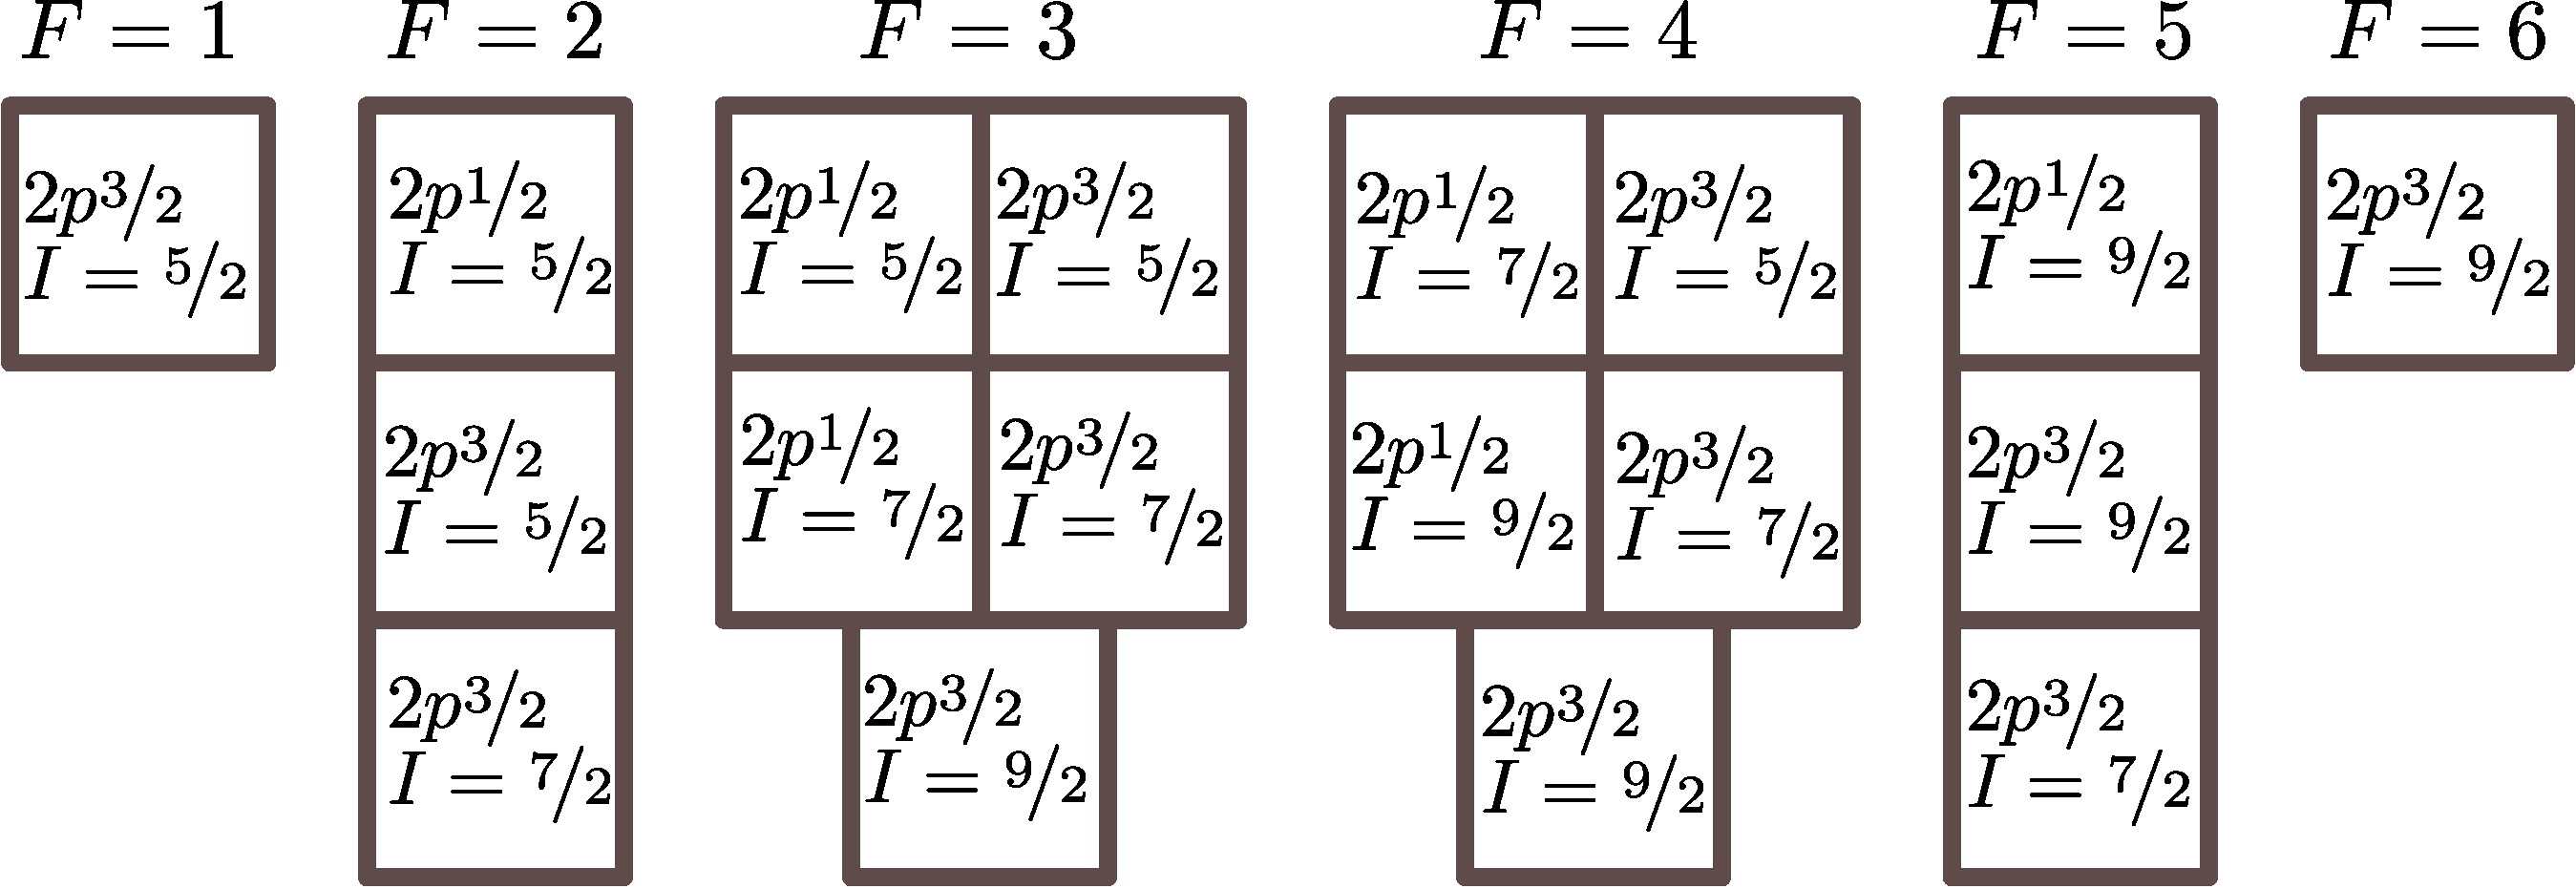
\includegraphics[width=0.91\linewidth]{pics/blocksRe.pdf}%
\caption{Separation of the modelspace consisting of the muonic $2p_{1/2}$ and $2p_{3/2}$ states coupled to the nuclear states with angular momentum $5/2$, $7/2$, and $9/2$. For every possible value of $F\in \{1,...,6\}$, the states are shown, which are involved in the rediagonalization of the hyperfine interaction.}%
\label{fig:blockRe}%
\end{figure}
%
%
\begin{figure}%
\centering
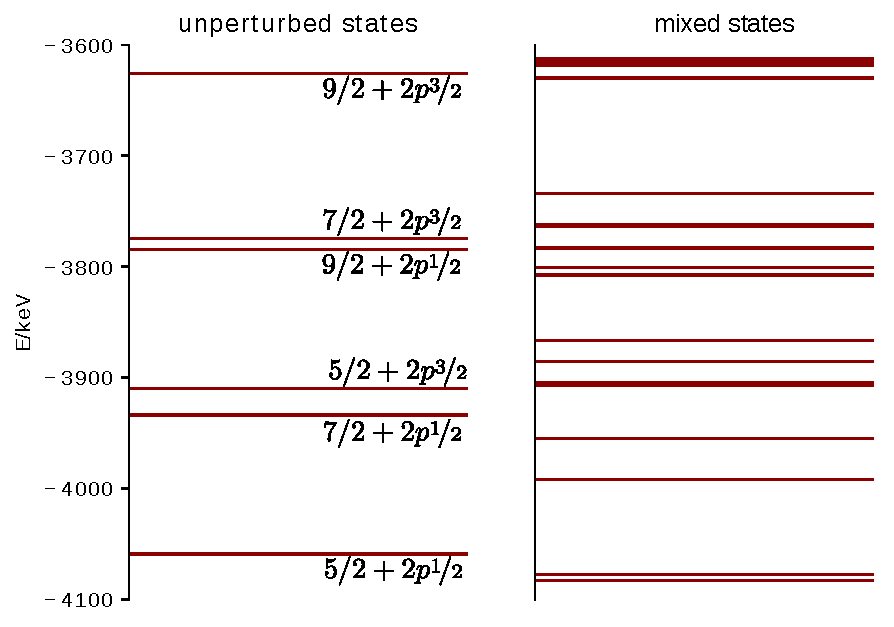
\includegraphics[width=0.75\linewidth]{pics/quad2.pdf}%
\caption{Level scheme of the muonic $2p_{1/2}$ and $2p_{3/2}$ states coupled to the nuclear 5/2, 7/2, and 9/2  states in $^{185}$Re. Zero energy corresponds to the free, resting muon and the nuclear ground state. Due to the nuclear rotational states and the strong quadrupole interaction, there is no clear distinction between fine- and hyperfine structure, which results in a rich structure of the energy levels.}%
\label{fig:quad2}%
\end{figure}
%

\subsection{Transition probabilities and intensities}
\label{sec:transitions}
It has been shown in Section~\ref{sec:muon_dynamic} that the coupling of muonic states and nuclear rotational states in connection with a strong quadrupole interaction leads to a rich and complicated level structure without a clear distinction of fine- and hyperfine structure. As a result, there is a large number of potential transitions between the states. For example, if the $L$ x-rays are considered, i.e. the transitions from the $3d$ fine-structure doublet to the $2p$ fine-structure doublet, there are only four transitions if the hyperfine structure is not considered. One of these transitions is suppressed because it is not an electric dipole transition. On the other hand, due to the dynamical hyperfine structure, there could be in principle hundreds of $L$ x-rays and many of them would be of electric dipole type. As a consequence, for the comparison with experimental spectra not only the level structure is needed, but also the corresponding relative intensities. In experimental spectra, the intensity of a transition is proportional to the number of measured photons with the energy of the transition. The intensities are a product of two quantities:
Firstly, it is proportional to the transition probability, which can be calculated, in principle, as soon as the wave functions and corresponding energies are known. In this thesis, the transition probabilities are calculated relativistically and without the long-wavelength approximation.
Secondly, the intensities are proportional to the population of the initial state. However, for the calculation of the population of the initial states, all transitions to the initial state from even higher states have to be considered. This eventually leads to a cascade calculation for the muon, where the muon is initially in a highly excited state and drops towards the ground state step-by-step by radiative transitions. In the following, the transition probabilities, the population, and the cascade calculations are discussed separately.\\

As a first step, the transition probabilities due to spontaneous emission of a photon in a muonic transition will be analyzed in this paragraph. Starting point is the general formula for the Einstein coefficient (transition probability per time) for a state with defined total angular momentum from an initial state $\left|F_iM_i,i_i\right>$ to a final state $\left|F_fM_f,i_f\right>$, where the states, in which the hyperfine structure is diagonalized, are defined in Eq.~\eqref{eq:rediagonState}. Following~\cite[Section 6.]{johnson2007}, this expression reads as
\begin{equation}
\label{eq:transitionGeneral}
A^{(\lambda)}_{J}=\frac{2\alpha (2J+1)(J+1)}{J}\Delta E_{if}\,\sum_{M,M_i,M_f} \left|\left<F_fM_f,i_f\middle|\hat{t}^{(\lambda)}_{JM}\middle|F_iM_f,i_i\right>\right|^2.
\end{equation}
Here, $\Delta E_{if}$ is the energy difference of the initial and final state, $J$ is the total angular momentum of the photon and $\lambda=1$ corresponds to an electric transition, whereas $\lambda=0$ stands for a magnetic transition. The multipole transition operator $\hat{t}^{(\lambda)}_{JM}$ is defined in Eqs.~(6.120), (6.121), (6.128), and (6.129) of Ref.~\cite{johnson2007} in terms of the components of the multipole potential $\mathbf{a}^{(\lambda)}_{JM}$ and of the scalar potential $\varphi_{JM}$ as
\begin{equation}
\boldsymbol{\alpha}\cdot \mathbf{a}^{(\lambda)}_{JM}(\mathbf{r}_\mu) - \varphi_{JM}(\mathbf{r}_\mu) = i\sqrt{\frac{(2J+1)(J+1)}{4\pi J}}\hat{t}^{(\lambda)}_{JM}(\mathbf{r}_\mu).
\end{equation}
Using Eq.~\eqref{eq:rediagonState} for the definition of the mixed states is terms of the unperturbed states $\left| FM_F\,IK\,n\kappa\right>$, the matrix elements are written as
\begin{equation}
\label{eq:tranElement1}
\left<F_fM_f,i_f\middle|\hat{t}^{(\lambda)}_{JM}\middle|F_iM_f,i_i\right> =
\sum_{k_i,\,k_f}\alpha^{(i_f)\,*}_{k_f} \alpha^{(i_i)}_{k_i}\left<F_fM_f\,I_{k_f}K\,n_{k_f}\kappa_{k_f} \middle|\hat{t}^{(\lambda)}_{JM}\middle|F_iM_i\,I_{k_i}K\,n_{k_i}\kappa_{k_i}\right>.
\end{equation}
Since the muonic transitions are considered in this section, the transition operator acts on the muonic coordinates~$\mathbf{r}_\mu$ only. These despribe one subsystem of the composite states in Eq.~\eqref{eq:transitionGeneral} with total angular momentum $F_i$ and $F_f$, respectively. Since the multipole transition operator is an irreducible tensor operator of rank $J$, Eq.~\eqref{app:subsystem_expectation} can be used for the computation of the matrix elements. This results in the following expression for the matrix elements:
\begin{alignat}{2}
\left<F_fM_f\,I_{k_f}K\,n_{k_f}\kappa_{k_f} \middle|\hat{t}^{(\lambda)}_{JM}\middle|F_iM_i\,I_{k_i}K\,n_{k_i}\kappa_{k_i}\right>=\delta_{I_{k_f}I_{k_i}}(-1)^{F_i+j(\kappa_{k_f})+I_{k_i}-J}
\notag\\[7.5pt]
\times\sqrt{2F_i+1}\text{C}^{F_fM_f}_{F_iM_i\,JM}
\begin{Bmatrix}
j(\kappa_{k_i})&j(\kappa_{k_f})&J\\
F_f&F_i&I_{k_i}
\end{Bmatrix}
\left< n_{k_f}\kappa_{k_f}\middle|\middle|\hat{t}^{(\lambda)}_{J}\middle|\middle|n_{k_i}\kappa_{k_i}\right>.
\label{eq:tranElement2}
\end{alignat}
The only dependency on the projection numbers $M$, $M_f$, and $M_i$ is in the arguments of the Clebsch-Gordan coefficients.
Furthermore, the Clebsch-Gordan coefficients in Eq.~\eqref{eq:tranElement2} do not depend on the summation indices $k_i$ and $k_f$.
Therefore, the summation over $M$, $M_f$, $M_i$ only affects the Clebsch-Gordan coefficients and the sum rule~\cite{varshalovich1988}
\begin{equation}
\sum_{M,M_i,M_f}\left(C^{F_fM_f}_{F_iM_i\,JM}\right)^2 = 2F_f+1
\end{equation}
can be used to simplify the calculation of Eq.~\eqref{eq:transitionGeneral} considerably. According to Ref.~\cite{johnson2007}, the reduced matrix elements in the muonic variables in Eq.~\eqref{eq:tranElement2} can be evaluated in length gauge as
\begin{alignat}{2}
\label{eq:relElTrans}
&\left< n_{f}\kappa_{f}\middle|\middle|\hat{t}^{(1)}_{J}\middle|\middle|n_{i}\kappa_{i}\right>=&&
\left<n_f\kappa_f\middle|\middle|C_J\middle|\middle|n_i\kappa_i\right>\\
&&&\times\int\text{d}r\,r^2 \text{\huge\{}j_J(\Delta E_{if}\,r)\left[g_{n_f\kappa_f}(r)g_{n_i\kappa_i}(r)+f_{n_i\kappa_i}(r)f_{n_f\kappa_f}(r)\right]\\
&&& +j_J(\Delta E_{if}\,r)\text{\huge[}\frac{\kappa_i-\kappa_f}{J+1}
\left(g_{n_f\kappa_f}(r)f_{n_i\kappa_i}(r)+g_{n_i\kappa_i}(r)f_{n_f\kappa_f}(r)\right)\\
&&& +\left(g_{n_i\kappa_i}(r)f_{n_f\kappa_f}(r)-g_{n_f\kappa_f}(r)f_{n_i\kappa_i}(r)\right)
 \text{\huge]}\text{\huge\}}
\end{alignat}
for electric transitions with $\lambda= 1 $ and as
\begin{alignat}{2}
\label{eq:relMagTrans}
&\left< n_{f}\kappa_{f}\middle|\middle|\hat{t}^{(0)}_{J}\middle|\middle|n_{i}\kappa_{i}\right>=&&
\left<n_f\,({-}{\kappa_f})\middle|\middle|C_J\middle|\middle|n_i\kappa_i\right>\notag\\
&&&\times\int\text{d}r\,r^2\frac{\kappa_i+\kappa_f}{J+1}j_J(\Delta E_{if}\,r)\left[-g_{n_f\kappa_f}(r)f_{n_i\kappa_i}(r)-f_{n_f\kappa_f}(r)g_{n_i\kappa_i}(r)\right]
\end{alignat}
for magnetic transitions with $\lambda = 0$. Here, $j_J(x)$ are the spherical Bessel functions~\cite[Eq. 10.47.3]{NIST:DLMF}.
The reduced matrix elements of the normalized spherical harmonics $\text{C}_{JM}(\vartheta,\varphi)$ read as~\cite{johnson2007}
\begin{alignat}{2}
&\left<n_f\kappa_f\middle|\middle|C_J\middle|\middle|n_i\kappa_i\right>=&&(-1)^{j(\kappa_f)+1/2}\sqrt{(2j(\kappa_i)+1)(2j(\kappa_f)+1)}\notag\\
&&& \times \pi(l(\kappa_f)+l(\kappa_i)+J)\,
\begin{pmatrix}
j(\kappa_f)&j(\kappa_i)&J\\
-\nicefrac{1}{2}&\nicefrac{1}{2}&0
\end{pmatrix},
\label{eq:reducedCjmuonic}
\end{alignat}
where the function $\pi(x)$ is defined in Eq.~\eqref{eq:parityFunc}. The angular momentum selection rules are implemented in the 6j- and 3j-symbols and in the function $\pi(x)$ in Eqs.~\eqref{eq:tranElement2} and~\eqref{eq:reducedCjmuonic}. For electric dipole transitions with $J=1$ and $\lambda=1$, the following selection rules have to be fulfilled:
\begin{alignat}{4}
&j(\kappa_i)&&=j(\kappa_f) &&\quad\text{ or }\quad j(\kappa_i)&&=j(\kappa_f)\pm 1,\\
&F_i &&= F_f &&\quad\text{ or }\quad\quad F_i&&=F_j\pm 1,\\
&l(\kappa_i)&&=l(\kappa_f)\pm 1.
\label{eq:dipoleSelectionRules}
\end{alignat}
The relativistic expression for the electric transitions in Eq.~\eqref{eq:relElTrans} can be simplified in the long-wavelength approximation. This neglects the effects of retardation. In this case, the lower component of the radial spinors $f_{n\kappa}(r)$ is small, and therefore mixed terms $f_{n_1\kappa_1}(r)g_{n_2\kappa_2}(r)$ can be neglected. The term $\sim f_{n\kappa}(r)^2$ is kept for convenience, since $r^2 g_{n\kappa}(r)^2+r^2 f_{n\kappa}(r)^2$ corresponds to the radial probability density. The long-wavelength approximation means, that $\Delta E_{if} \, r$ is small, and therefore the corresponding spherical Bessel function can be expanded. For small arguments, the spherical Bessel functions can be approximated as
\begin{equation}
j_J(x)\approx \frac{x^J}{(2J+1)!!},
\end{equation}
where the double factorial is evaluated as $n!! = n \cdot (n-2) \cdot (n-4) \cdot ...\,\,$. Thereby, Eq.~\eqref{eq:relElTrans} becomes
\begin{alignat}{2}
\label{eq:relElTransNR}
&\left< n_{f}\kappa_{f}\middle|\middle|\hat{t}^{(1)}_{J}\middle|\middle|n_{i}\kappa_{i}\right>=&&
\left<n_f\kappa_f\middle|\middle|C_J\middle|\middle|n_i\kappa_i\right>\\
&&&\times\frac{\Delta E_{if}^J}{(2J+1)!!}\int\text{d}r\,r^2 \;r^J\left(g_{n_f\kappa_f}(r)g_{n_i\kappa_i}(r)+f_{n_i\kappa_i}(r)f_{n_f\kappa_f}(r)\right),
\end{alignat}
and the corresponding transition probabilities per time from Eq.~\eqref{eq:transitionGeneral} thereby have the energy dependence dependence $\sim \Delta E_{if} ^{2J+1}$.\\

After the transition probabilities have been discussed in the last paragraph, the remaining issue of the population of the initial states is discussed in the following.
The transition probabilities can be calculated ab initio, independent from experimental details. Unfortunately, this is not the case for the population. Here, details of the experimental setup and the capture process have to be considered. Muonic atoms are typically created by shooting a slow muon beem on a target, which contains the isotope of interest~\cite{wu1969,Devons1995,BorieRinker1982}. The average population of the muonic states after the muon has been captured by the nucleus depends on the state of the incoming muon as well as details of the nuclear target. Additionally, for highly excited states, the muon and the atomic electrons are not well separated, as described in Section~\ref{sec:screen}, thus the muon-electron interaction has to be taken into account and for example Auger transitions can occur~\cite{pisano1982}. In heavy nuclei, this leads to a complicated many-body problem. Even if an initial population of the low-lying muonic states where the electron-muon interaction can be neglected would be known in form of the diagonal elements of the muonic density matrix, the master equation using transition probabilities as given in Eqs.\eqref{eq:relElTrans} and \eqref{eq:relMagTrans} has to be solved~\cite{pisano1982}. Due to the large number of energy levels in the dynamical hyperfine structure and the calculation of the transition probabilities with Eq.~\eqref{eq:transitionGeneral}, this is still a very time-consuming calculation.

However, the cascade calculation can be simplified considerably. In experiments, muons typically tend to be captured in circular orbits, which are states with maximal angular momentum $l$=$n-1$. Additionally, the fastest transitions are electric dipole transitions of the muon, which change the orbital angular momentum quantum number of the muon by one. The most probable sequence of transitions correspondingly is: $5g\rightarrow 4f \rightarrow 3d \rightarrow 2p \rightarrow 1s$. Especially the $2p\rightarrow 1s$ ($K$ x-rays) and $3d\rightarrow 2p$ ($L$ x-rays) spectra have been used in the past to obtain information about nuclear structure from experiments with muonic atoms, e.g. in Refs.~\cite{tanaka1983,tanaka1984,tanaka1984_2,hitlin1970,Dey1979,dewit1966,Bergem1988}. Under the assumption that the muon starts in a circular orbit and then cascades by electric dipole transitions, the calculation of the intensities is considerably simplified. Because of the selection rules from Eq.~\eqref{eq:dipoleSelectionRules}, the $2p$ state can be only populated by the $3d$ states, which can only be populated by the $4f$ states and so on. This approach for the cascade calculations will be used also in this thesis. The population of a state in the, say, $2p$ states can be obtained by summing up all intensities of the transitions from the $3d$ states to this state. Finally, only the initial population of the initial states with the highest $n$ needs to be given. Here, a simple statistical population has proved to describe experiments correctly~\cite{Dey1979}, where every coupled muon-nucleus state with total angular momentum $F$ has a relative population $\sim (2F+1)$, corresponding to the different $M_F$ values. Furthermore, initially the nucleus is in its ground state, since the excitation of nuclear rotational levels only occurs during the muonic cascade, when energy is transfered from the muon to the nucleus.
The cascade starting from the muonic $4f$ states is visualized in Fig.~\ref{fig:cascade}. In practice, the calculation of the spectrum begins with the diagonalization the hyperfine interaction in the fine-structure doublets of the states with circular orbits ($2p$, $3d$, $4f$). Then, under the assumption of a relative population proportional to $(2F+1)$ in the fine-structure doublet with the highest quantum number $n=n_{\text{max}}$, all transitions to the next states with $n_{\text{max}-1}$ are calculated. The relative population of the $n_{\text{max}-1}$ states is obtained by summing up the intensities of all transitions to this state. This procedure can be repeated until the muonic ground state is reached, and thereby all line-intensities are obtained. A statistical population $\sim (2F+1)$ in the higher states leads to a statistical population in the lower states, as long as the hyperfine-structure  splitting can be neglected. In states with $n>3$, the hyperfine-structure splitting is typically small. Therefore, statistically populated $6h$ states lead to (almost) statistically populated $5g$, which in turn result in (almost) statistically populated $4f$ states. Thereby, the line intensities are in practice insensitive on the starting point of the cascade. The calculation of transition probabilities is used in Section~\ref{sec:muon_re} for the analysis of the spectrum of muonic rhenium.
%
\begin{figure}%
\centering
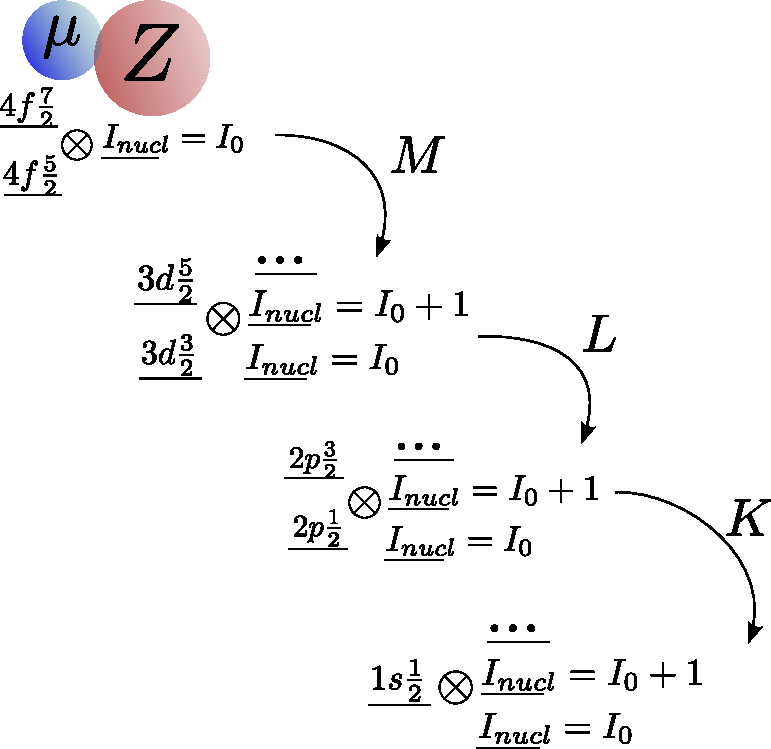
\includegraphics[width=0.82\linewidth]{pics/cascade.pdf}%
\caption{Visualization of the muonic cascade, starting from the muonic $4f$ states and the nucleus in its ground state. Then, the muon is cascading towards its ground state through the $3d$ and $2p$ states. Here, excited nuclear rotational states can be populated. The population of a state in the $3d$ modelspace is obtained by summing up all transitions from the $4f$ states to this state, and analogously for the $2p$ states. For a given initial population of the $4f$ states, in this way all intensities can be calculated.}%
\label{fig:cascade}%
\end{figure}
%
\newpage
\section{Higher order corrections for the dynamical hyperfine structure}
\label{sec:higherorder}
In this section, improved calculations of two higher order contributions to the dynamical hyperfine structure are discussed. Firstly, corrections of the quadrupole matrix elements due to vacuum polarization (VP) are considered. Furthermore, a numerical treatment of second order quadrupole interactions is presented.

The contribution of leading order VP to the spherically symmetric part of the charge distribution was briefly discussed in Section~\ref{sec:qed}. However, VP influences multipole interactions of all orders, thus in the context of the dynamical hyperfine structure it influences matrix elements of the quadrupole interaction between muon and nucleus. Until now, the corresponding correction to the matrix elements has only been considered with a power-series expansion~\cite{Fricke1969vp,zehnder1975} or for specific forms of the nuclear charge distribution~\cite{pearson1963}, which does not enable precision calculations for heavy muonic atoms. In this thesis, a new approach is developed in Section~\ref{sec:muon_quadUehl} by performing a multipole expansion of the Uehling potential. This enables the calculation of the leading order VP correction to the quadrupole matrix elements for arbitrary charge distributions with all finite size effects.

The approach of quasi-degenerate perturbation theory is discussed in Section~\ref{sec:almostDeg}, and the rediagonalization of the perturbation is applied to the hyperfine interaction in Section~\ref{sec:non-diagElements} and~\ref{sec:toyModelRediag}. However, there are residual second order corrections due to contrubutions from outside of the modelspace, as introduced in Eq.~\eqref{eq:pert_secondOrderEnerg}. A non-relativistic estimation of the residual second order electric quadrupole interaction with states outside of this modelspace has been presented in Ref.~\cite{chen1970}. In this thesis, an extended, fully relativistic approach is presented in Section~\ref{sec:muon_residualSO}.

\subsection{Quadrupole-Uehling interactions}
\label{sec:muon_quadUehl}
The resummation of the order $\alpha (Z\alpha)$ VP (Uehling potential) has been discussed in Section~\ref{sec:vacPolTheory}, with the result that it can be included in the Dirac equation. The starting point of this section is the renormalized expression for the Uehling potential for a given deformed nuclear charge distribution, which reads in the chosen system of units (Appendix~\ref{app:conventions}) as~\cite{Fullerton1976}
\begin{equation}
{V_{\text{uehl}}(\mathbf{r}_\mu^{\,\prime})}{=}{-Z\alpha\frac{2 \alpha}{3\pi} \int \text{d}^3\mathbf{r}_N^{\prime} \frac{\rho(\mathbf{r}_N^{\,\prime})}{|\mathbf{r}_\mu^{\,\prime} - \mathbf{r}_N^{\,\prime}\,|} K_1(2m_e{|\mathbf{r}_\mu^{\,\prime} - \mathbf{r}_N^{\,\prime}\,|}),}
\label{eq:Vvp}
\end{equation}
where $m_e$ is the electron mass, and primed coordinates belong to the body-fixed nuclear system, as defined in~\ref{sec:muon_framework}. $K_1(x)$ belongs to the family of functions
\begin{equation}
K_n(x)=\int_1^\infty \text{d}t\,\text{e}^{-xt}\left(\frac{1}{t^3}+\frac{1}{2t^5}\right)\sqrt{t^2-1}t^n.
\label{eq:defKn}
\end{equation}
For different $n$, the functions $K_n(x)$ are related by
\begin{alignat}{2}
&K_n(x)&&=-\partial_x K_{n-1}(y),\\
&K_{n-1}(x)&&=-\int^x\text{d}y\, K_n(y).
\label{eq:Kninfo}
\end{alignat}
Furthermore, they can be expressed in terms of Meijer G functions from Eq.~\eqref{app:def_meijerG} as
\begin{equation}
K_n(x)=\frac{1}{4} {G_{1, 3}^{3, 0}\left({\frac{x^{2}}{4}}\middle|\begin{matrix}   - \frac{n}{2} + 2 \\- \frac{n}{2} + \frac{1}{2}, 0, \frac{1}{2}   \end{matrix}   \right)} + \frac{1}{8} {G_{1, 3}^{3, 0}\left(\frac{x^2}{4}\middle| \begin{matrix}   - \frac{n}{2} + 3 \\- \frac{n}{2} + \frac{3}{2}, 0, \frac{1}{2}   \end{matrix}  \right)},
\label{eq:defKnAnalyt}
\end{equation}
which makes it possible to evaluate them with arbitrary precision implementations of the Meijer G function in existing libraries or programs like Refs.~\cite{Mathematica,mpmath}. The Uehling potential~\eqref{eq:Vvp} depends only on $|\mathbf{r}_\mu^{\,\prime} - \mathbf{r}_N^{\,\prime}\,|$, similar to the electric potential~\eqref{eq:defmulti}, which can be written as
\begin{equation}
|\mathbf{r}_\mu^{\,\prime} - \mathbf{r}_N^{\,\prime}|
=|\mathbf{r}_\mu - \mathbf{r}_N|
=\sqrt{r_\mu^2 + r_N^2 - 2 r_\mu r_N y},
\end{equation}
and therefore only depends on the lengths of the vectors and on ${y}{=}{\cos(\sphericalangle \mathbf{r}_\mu\mathbf{r}_N)}$. The dependence on $|\mathbf{r}_\mu^{\,\prime} - \mathbf{r}_N^{\,\prime}\,|$ is more complicated for the Uehling potential, but a multipole expansion can be performed nonetheless by expanding the dependence on $y$ in Legendre polynomials. It reads
\begin{alignat}{2}
&\frac{K_1(2m_e{|\mathbf{r}_\mu^{\,\prime} - \mathbf{r}^{\,\prime}\,|})}{|\mathbf{r}_\mu^{\,\prime} - \mathbf{r}^{\,\prime}\,|}
&&=\sum_{l=0}^\infty c_l(r_\mu,r_N) P_l(y)\\
&&&=\sum_{l=0}^\infty c_l(r_\mu,r_N) \sum_{m=-l}^l \text{C}^*_{lm}(\vartheta_N^{\prime},\varphi_N^{\prime})\text{C}_{lm}(\vartheta_\mu^\prime,\varphi_\mu^\prime),\notag
\end{alignat}
where the second equality is a consequence of the addition theorem~\eqref{eq:legendreAddTheorem} of Legendre polynomials. The expansion coefficients are still functions of the lengths of the vectors and are defined as
\begin{equation}
c_l(r_\mu,r_N)=\frac{2l+1}{2} \int_{-1}^1 \text{d}y \frac{K_1(2m_e{|\mathbf{r}_\mu - \mathbf{r}_N|})}{|\mathbf{r}_\mu - \mathbf{r}_N|} P_l(y).
\label{eq:defcl}
\end{equation}
Eq.~\eqref{eq:defcl} can be either solved by numerical integration, or expressed in a closed form, using Eq.~\eqref{eq:defKnAnalyt} for the functions $K_n(x)$. For the closed form expression, the integration variable $y$ in Eq.~\eqref{eq:defcl} is substituted by $z=f^{-1}(y)=2m_e{|\mathbf{r}_\mu - \mathbf{r}_N|}$ or $y=f(z)=(r_\mu^2+r_N^2 -(z/2m)^2)/(2r_\mu r_N)$. Thereby, Eq.~\eqref{eq:defcl} reads as
\begin{equation}
c_l(r_\mu,r_N)=\frac{2l+1}{4 r_\mu r_N m_e}\mathop\int\limits_{2m_e{|r_\mu - r_N|}}^{2m_e{(r_\mu + r_N)}} \text{d}z\, K_1(z)P_l(f(z)).
\label{eq:defcl2}
\end{equation}
Since $f(z)$ is quadratic in $z$, it follows that $P_l(f(z))$ is a polynomial of degree $2l$. Thereby, Eq.\eqref{eq:defcl2} can be integrated by part $2l$-times for the two functions $K_1(z)$ and $P_l(f(z))$, using the relations from Eq.~\eqref{eq:Kninfo}, to solve the integral as
\begin{equation}
c_l(r_\mu,r_N)=\frac{2l+1}{4 r_\mu r_N m_e}
\sum\limits_{i=0}^{2l} K_{-i}(z)\,\partial^{(i)}_yP_l(f(z))\text{\huge |}^{y=2m_e{|r_\mu - r_N|}}_{y=2m_e{(r_\mu + r_N)}}.
\label{eq:defcl3}
\end{equation}
Thereby, the Uehling potential can be written, analogously to the electric potential, as
\begin{align}
V_{\text{uehl}}(\mathbf{r}_\mu,\phi,\theta)=&\sum_{l=0}^\infty-Z\alpha\frac{2\alpha}{3\pi}
 \int \text{d}^3r^{\prime}_N c_l(r_\mu,r_N)\text{P}_{l}(\cos \vartheta_N^{\prime})\rho(\mathbf{r}_N^{\,\prime})\sum_{m=-l}^l \text{C}^*_{lm}(\theta,\phi)\text{C}_{lm}(\vartheta_\mu,\varphi_\mu).\notag\\
=:&\sum_{l=0}^\infty Q^{(l)}_{\text{uehl}}(r_\mu)\,\sum_{m=-l}^lC^*_{lm}(\theta,\phi)C_{lm}(\vartheta_\mu,\varphi_\mu)&\notag\\
=:& \sum_{l=0}^\infty V^{(l)}_{\text{uehl}}(\mathbf{r}_\mu,\phi,\theta).
\label{eq:defmultiuehl}
\end{align}
For $l=0$, the expression for Uehling potential of a spherical charge distribution~\cite{Fullerton1976} which only depends on $r_\mu$ is recovered as
\begin{align}
\label{eq:sph_uehl}
V^{(0)}_{\text{uehl}}(r_\mu)=& -\frac{2\alpha (Z\alpha)}{3 m_e r}\int_0^\infty \text{d}r^{\prime}\,\rho_0(r^\prime)\left[K_0(2m_e|r-r^\prime|)-K_0(2m_e(r+r^\prime))\right],
\end{align}
where the spherically averaged part of the charge distribution is
\begin{equation}
\rho_0(r)=\frac{1}{4\pi}\int_0^{2\pi}\text{d}\varphi\int_0^\pi\text{d}\vartheta \sin(\vartheta)\rho(\mathbf{r}).
\end{equation}
%
% begin quad uehl figure
\begin{figure}[t]%
\centering
\subfloat[]{\label{fig:quehl1}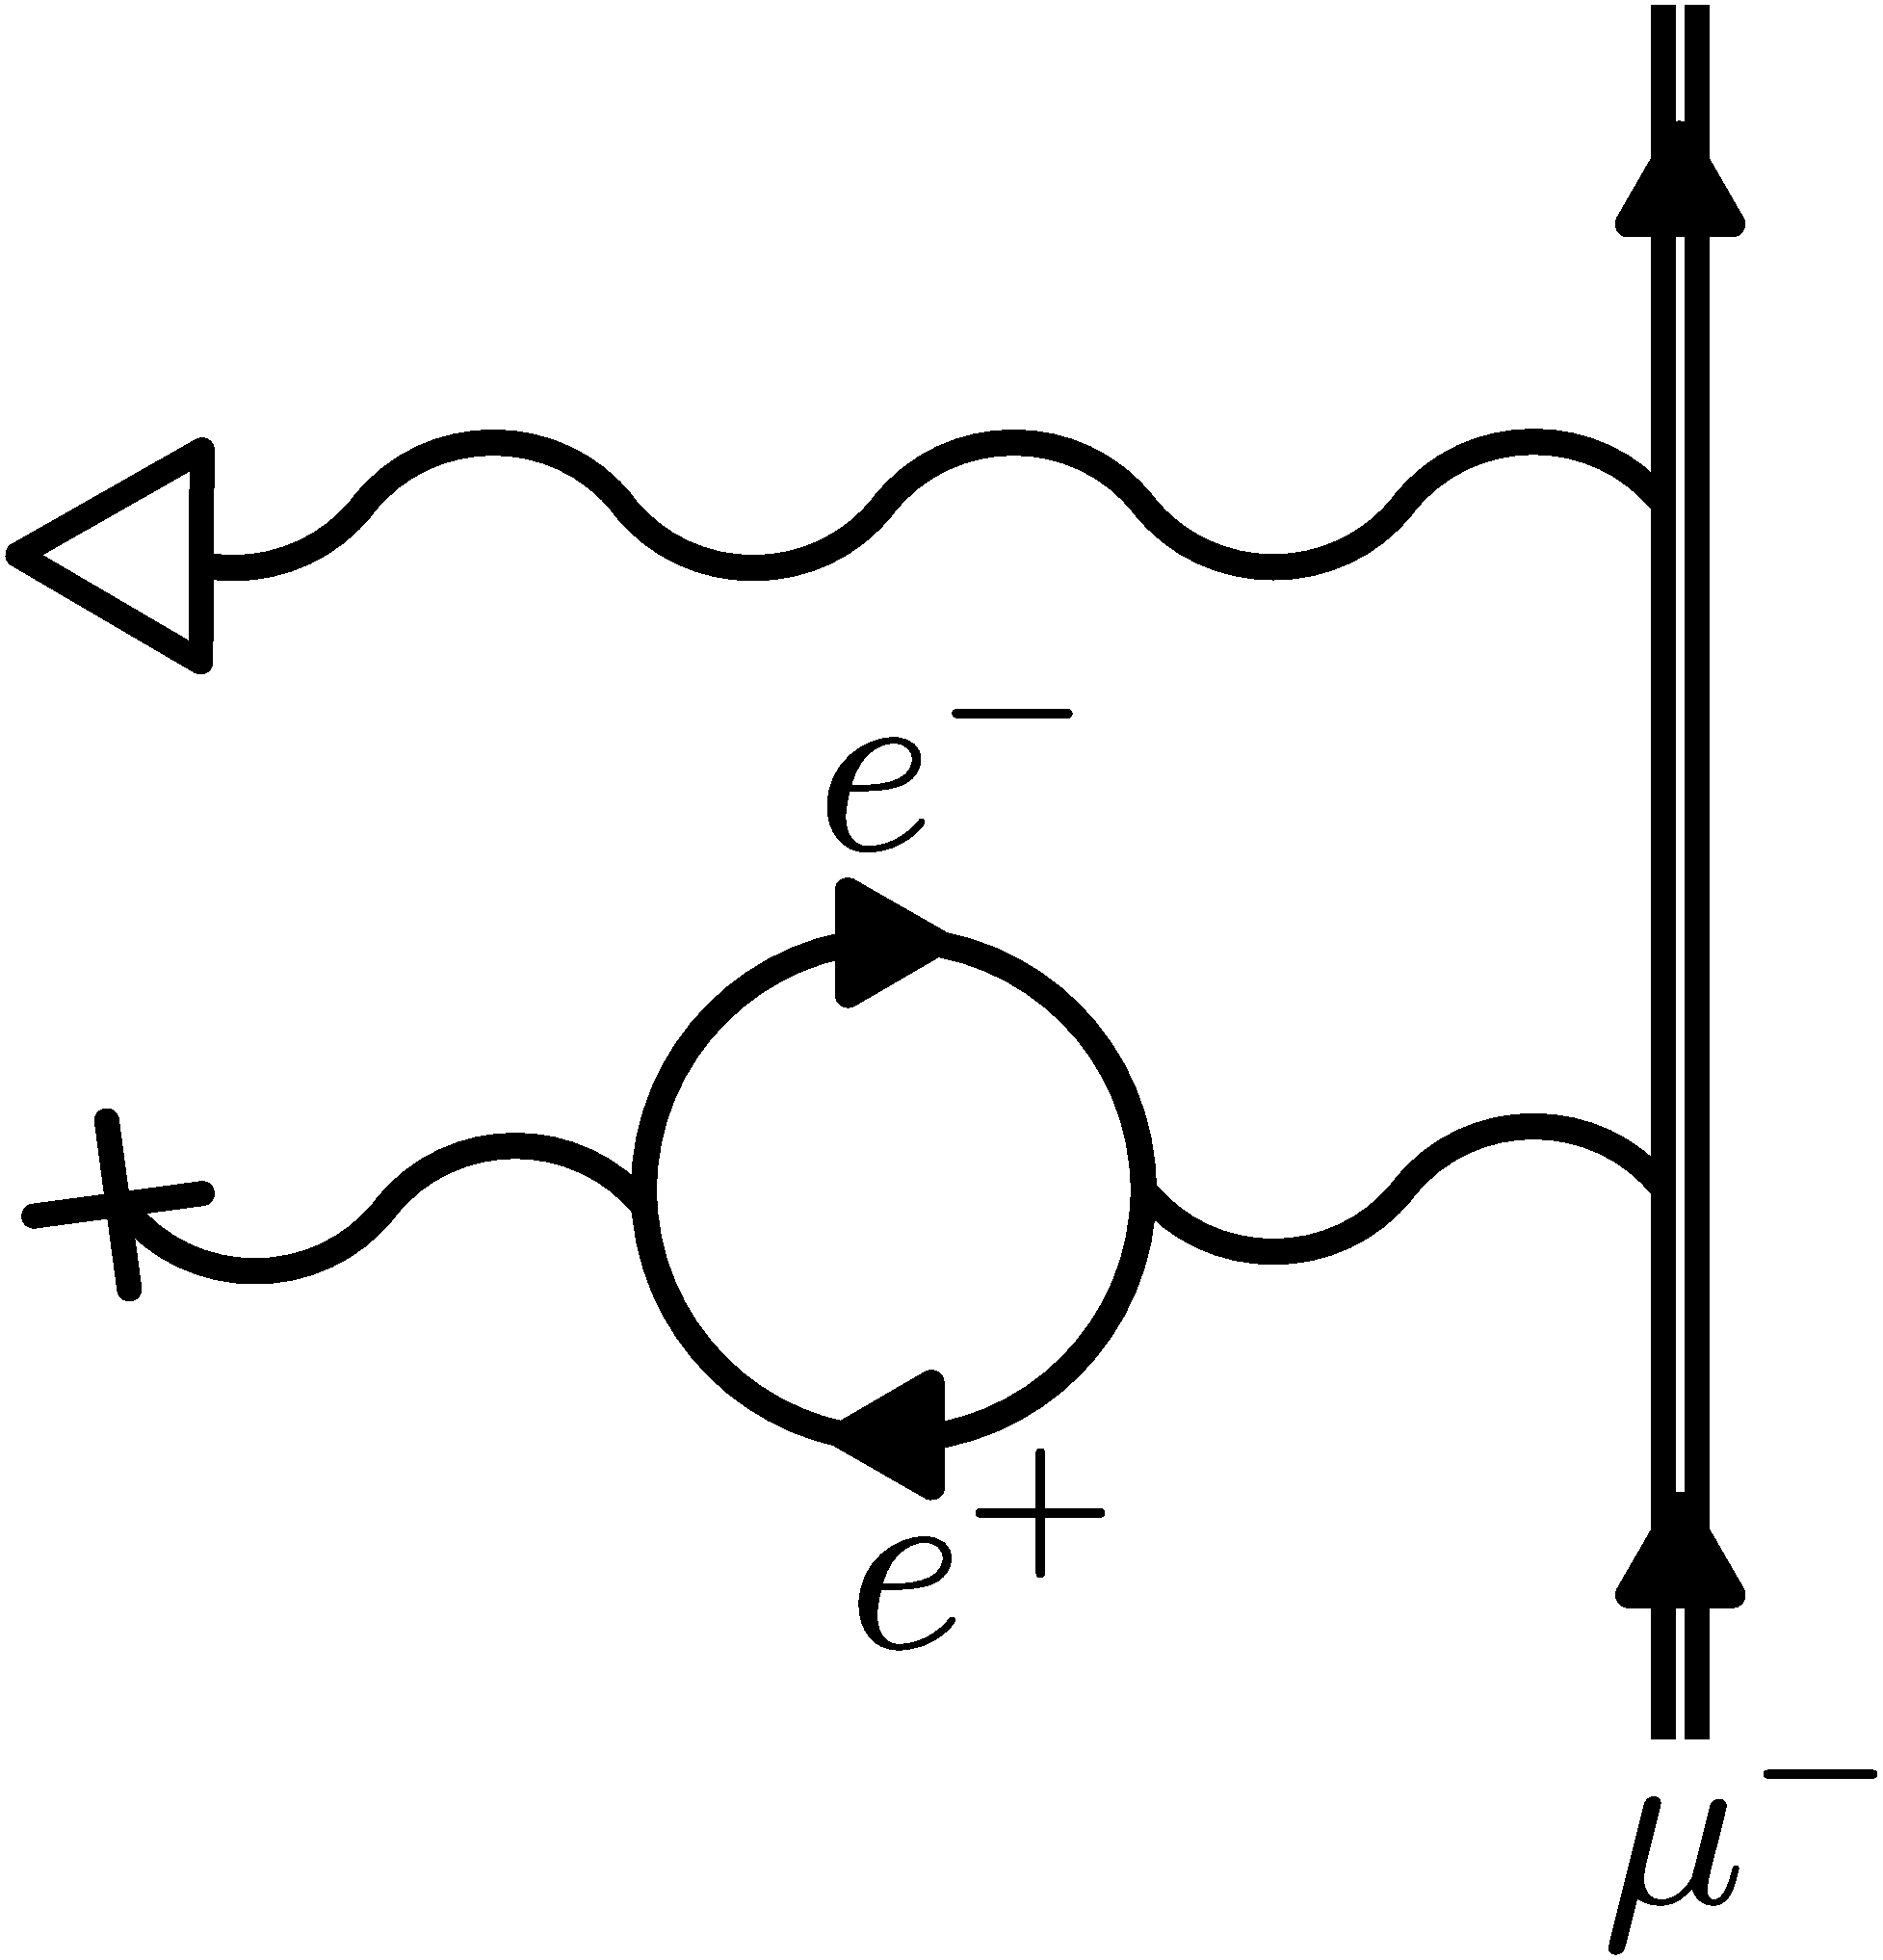
\includegraphics[width=0.3\linewidth]{pics/mixed}}
\hspace{2cm}
\subfloat[]{\label{fig:quehl2}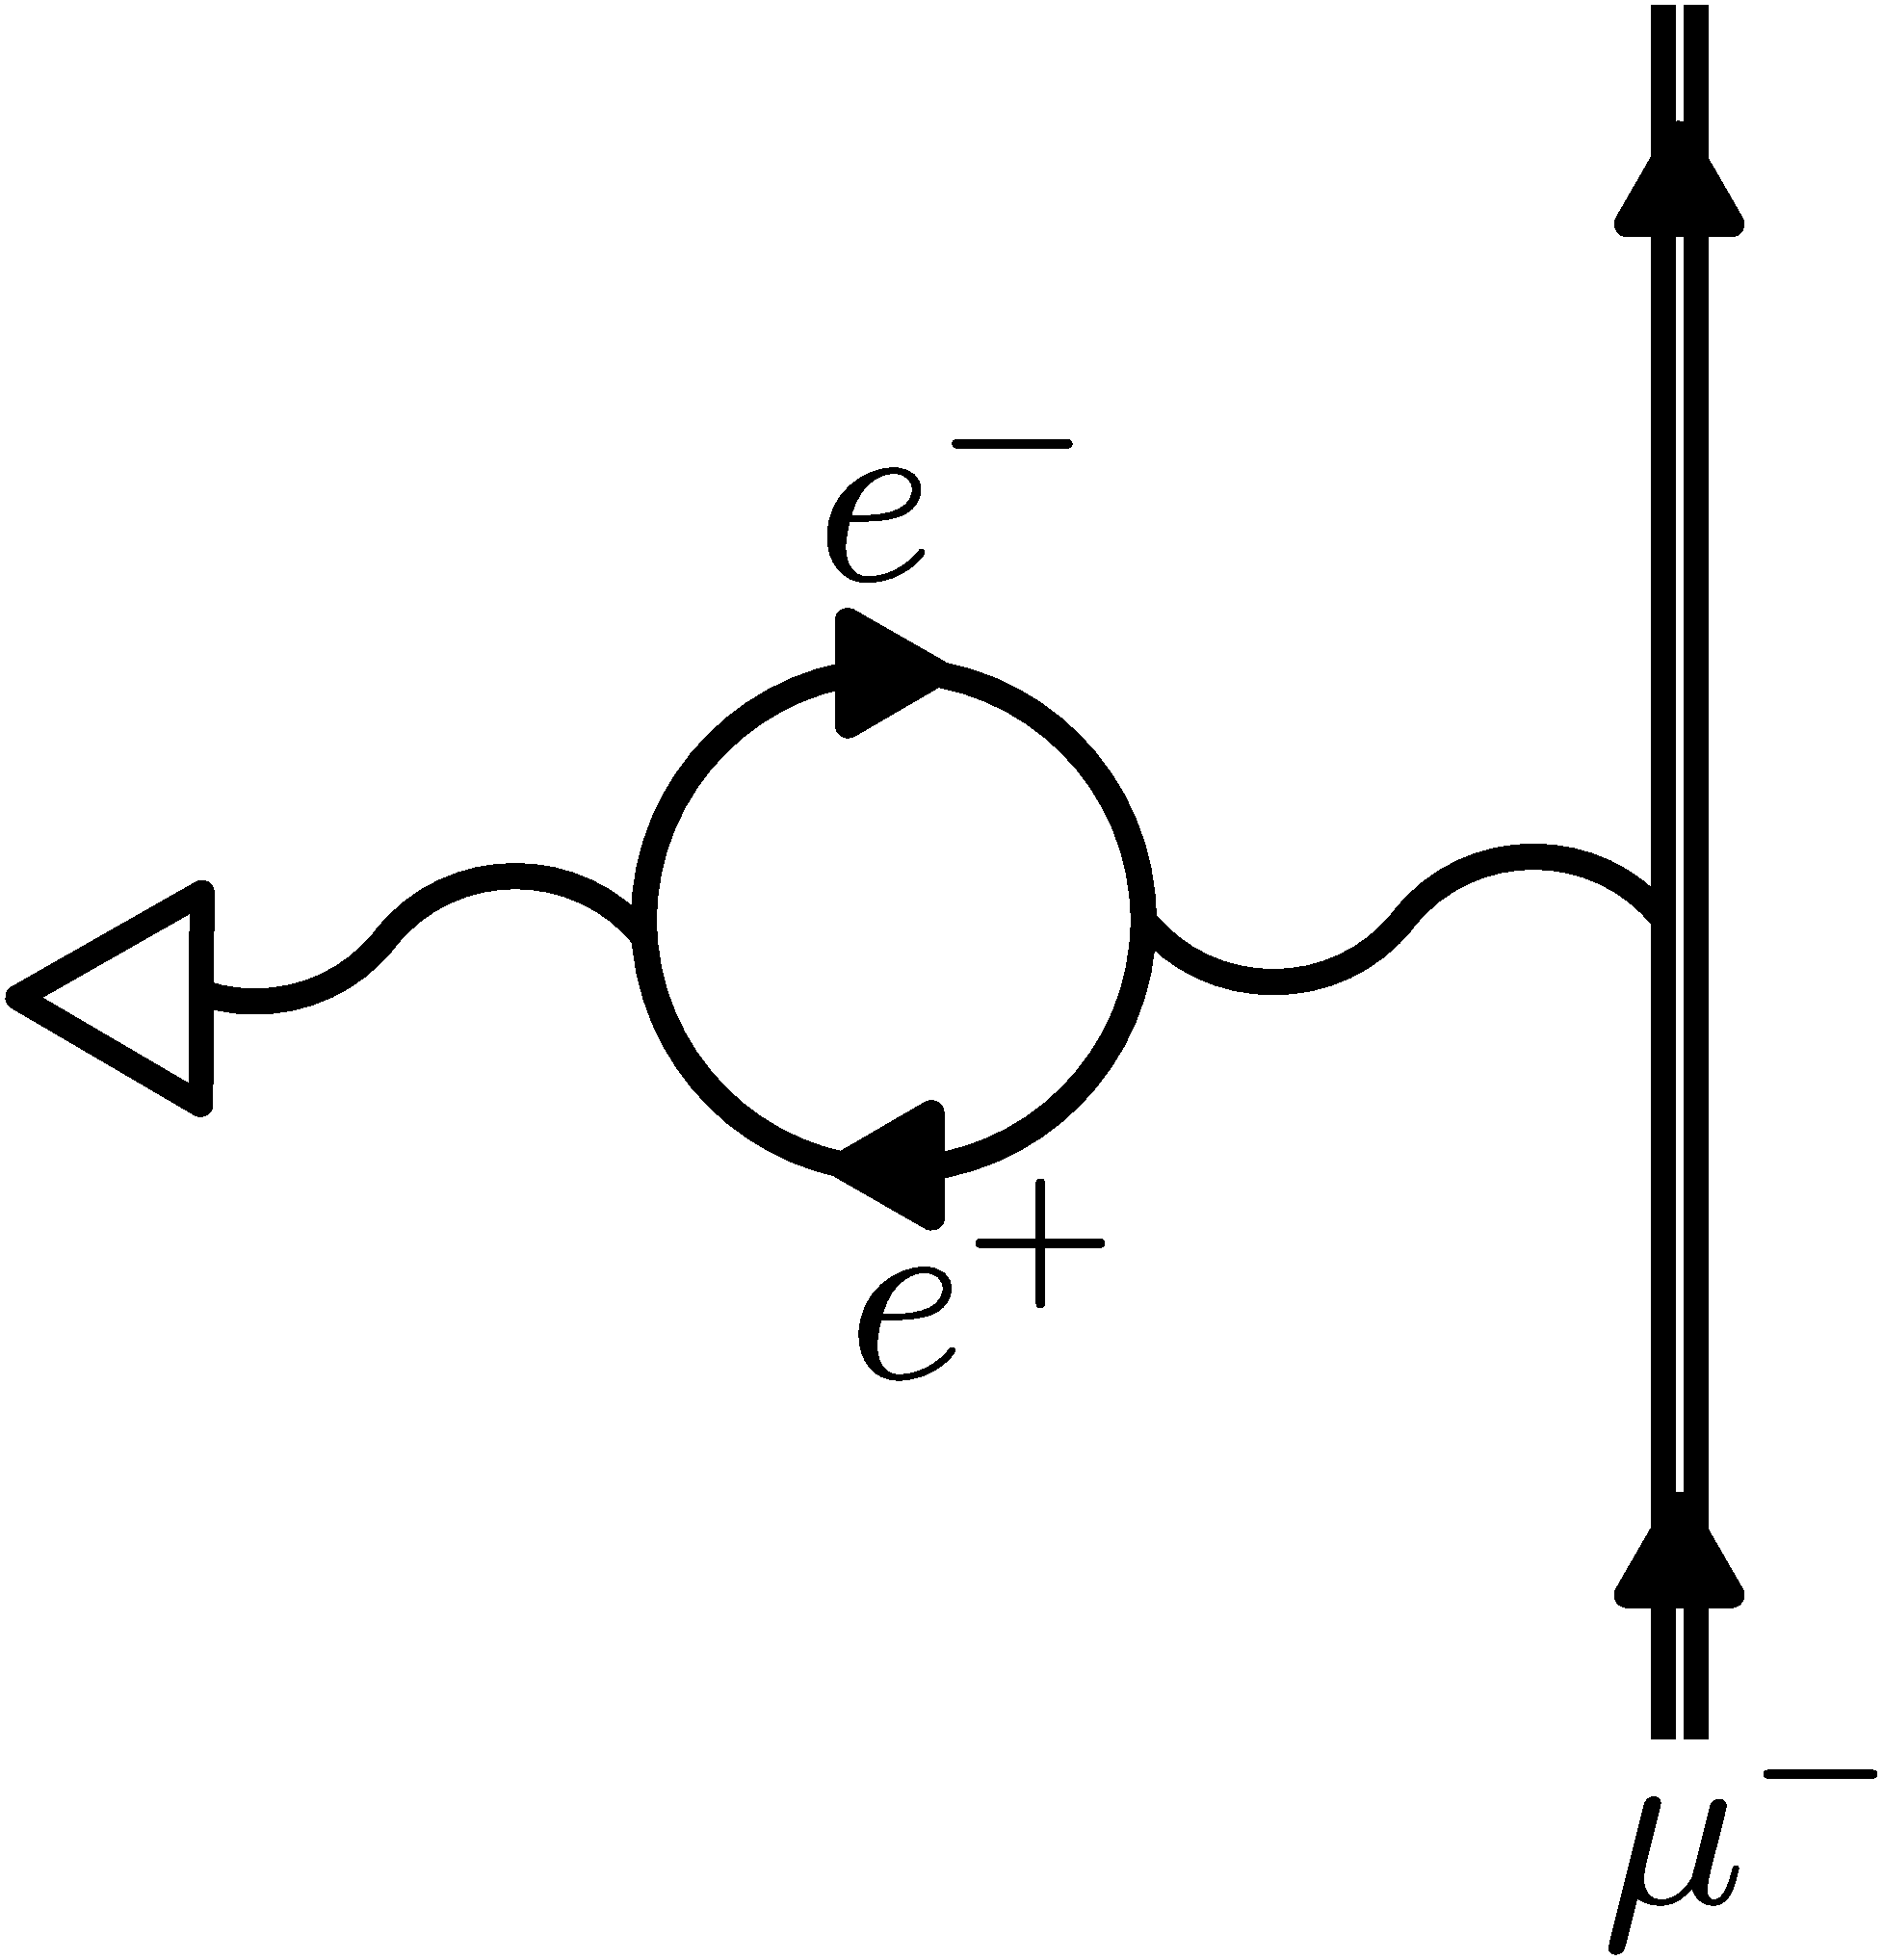
\includegraphics[width=0.3\linewidth]{pics/quehl}}
%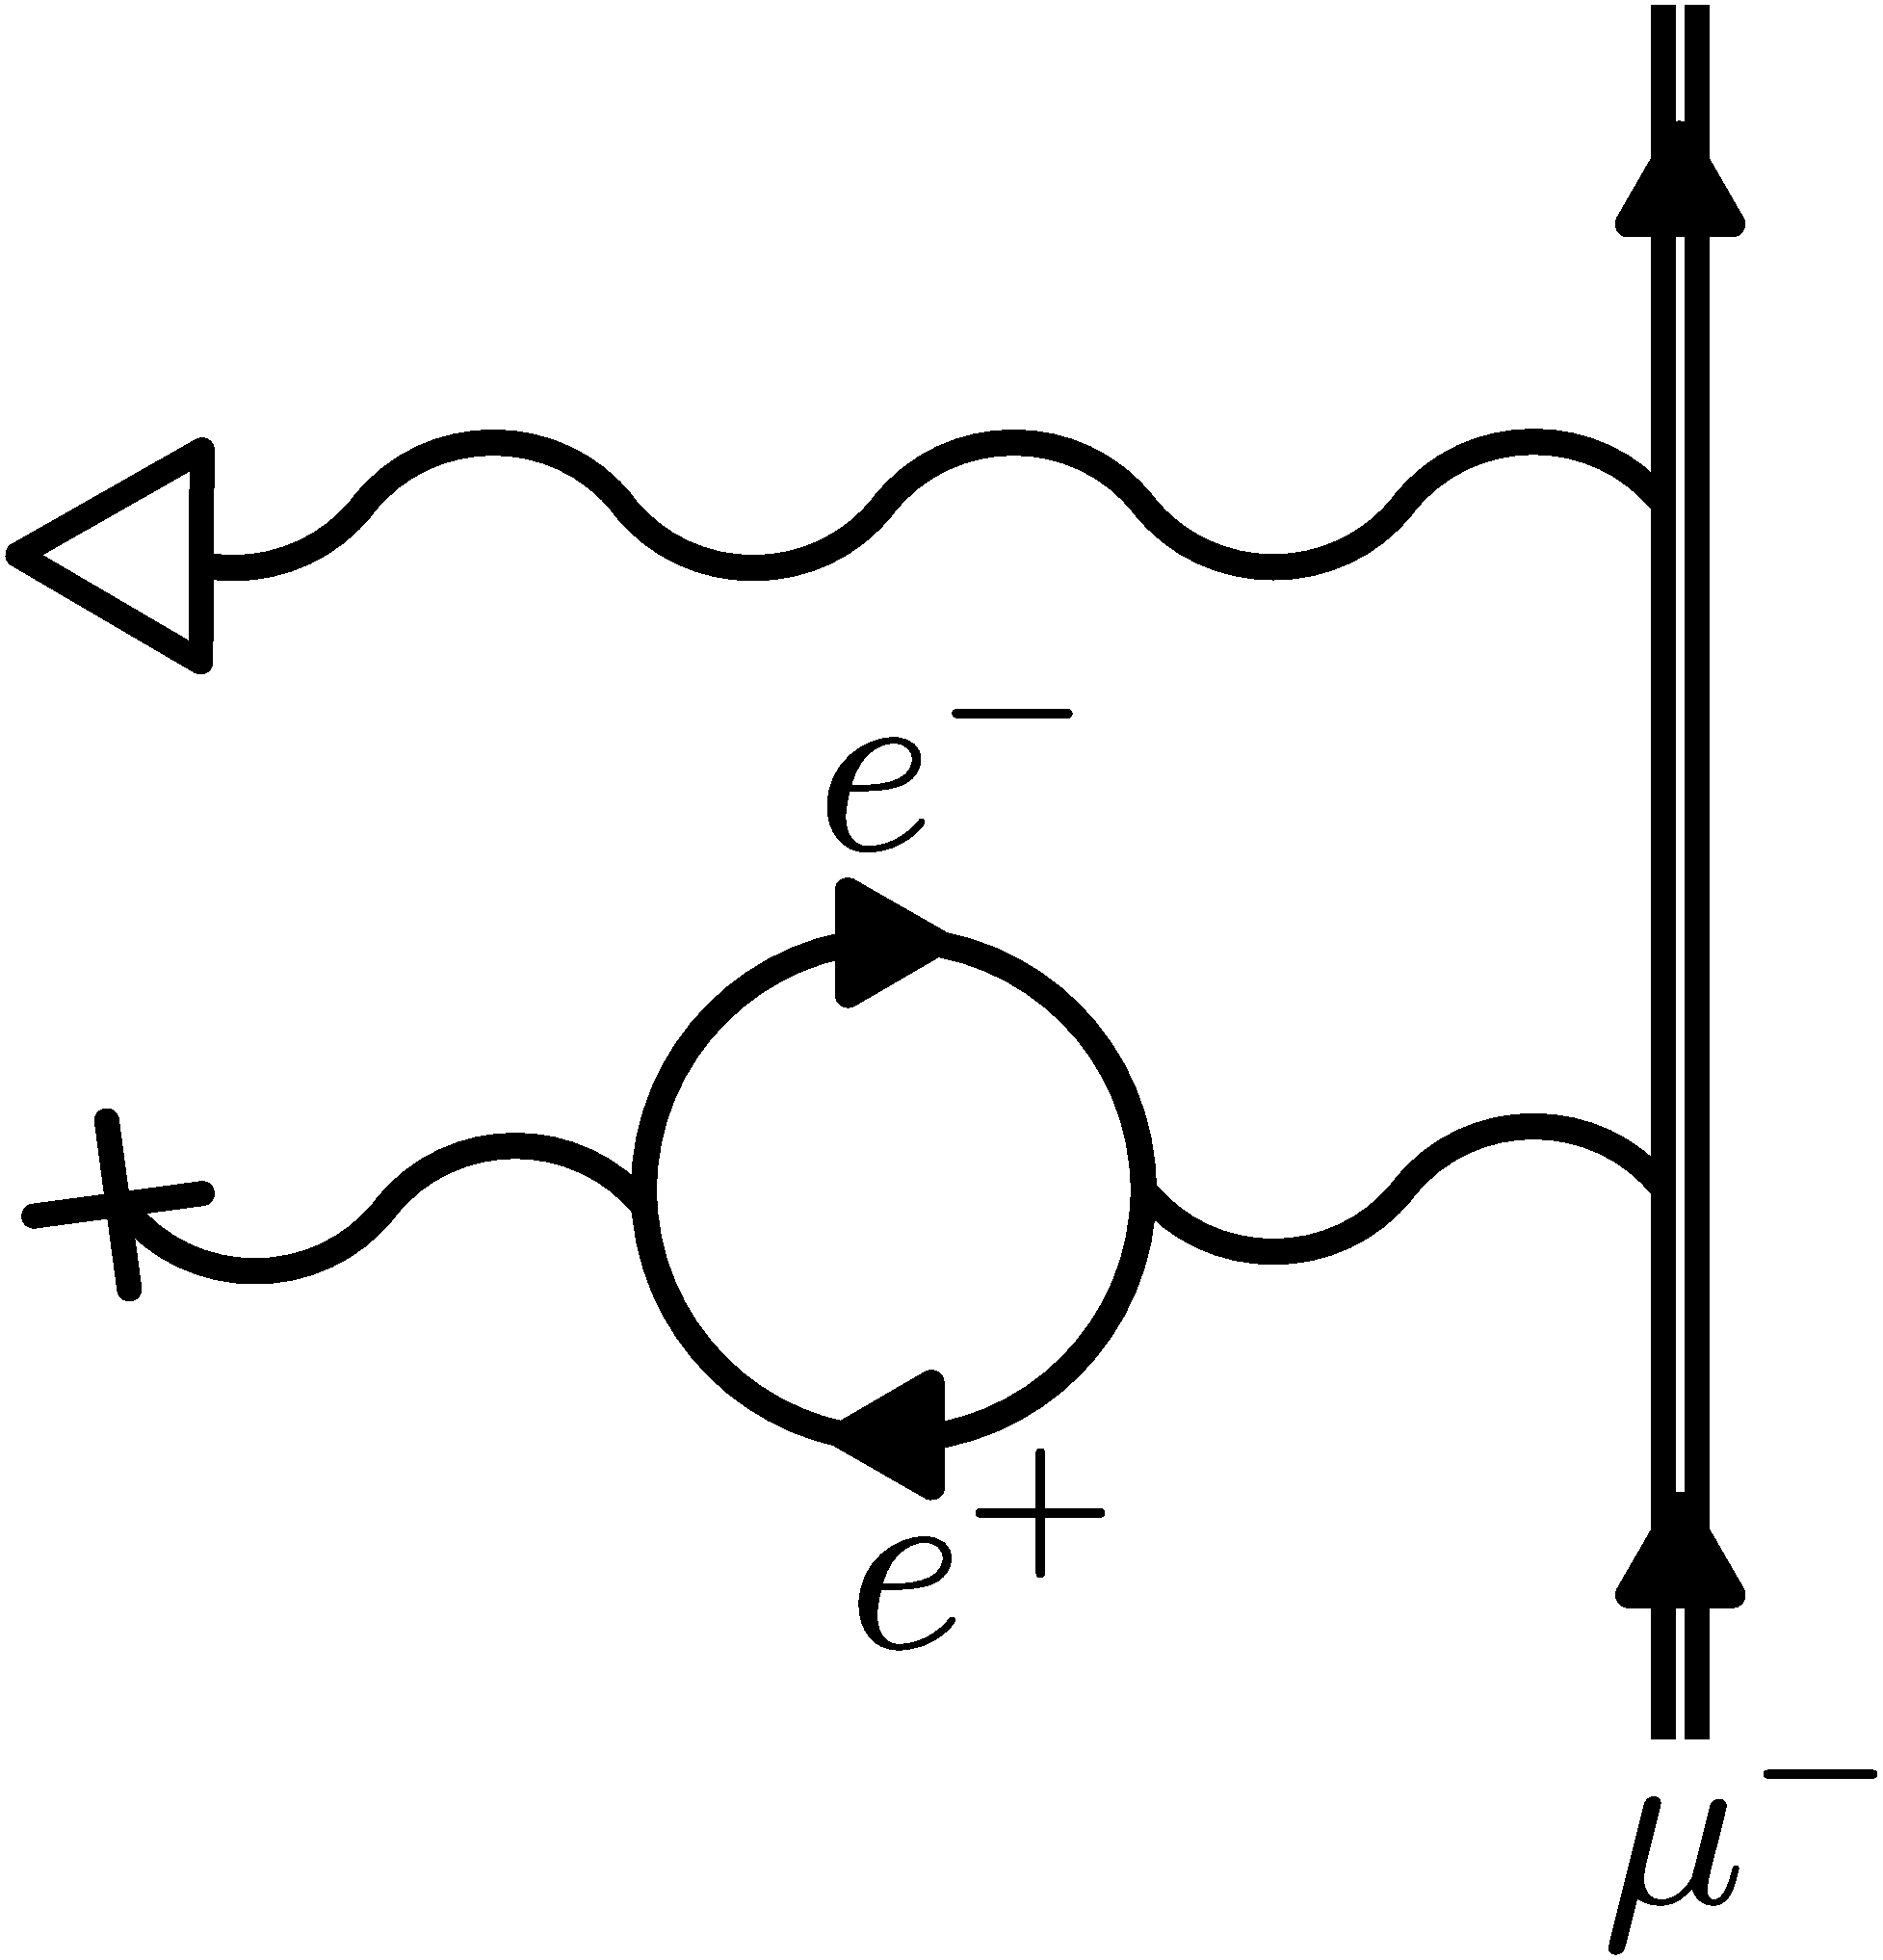
\includegraphics[width=0.30\textwidth]{pics/mixed}\hspace{3.5cm}
%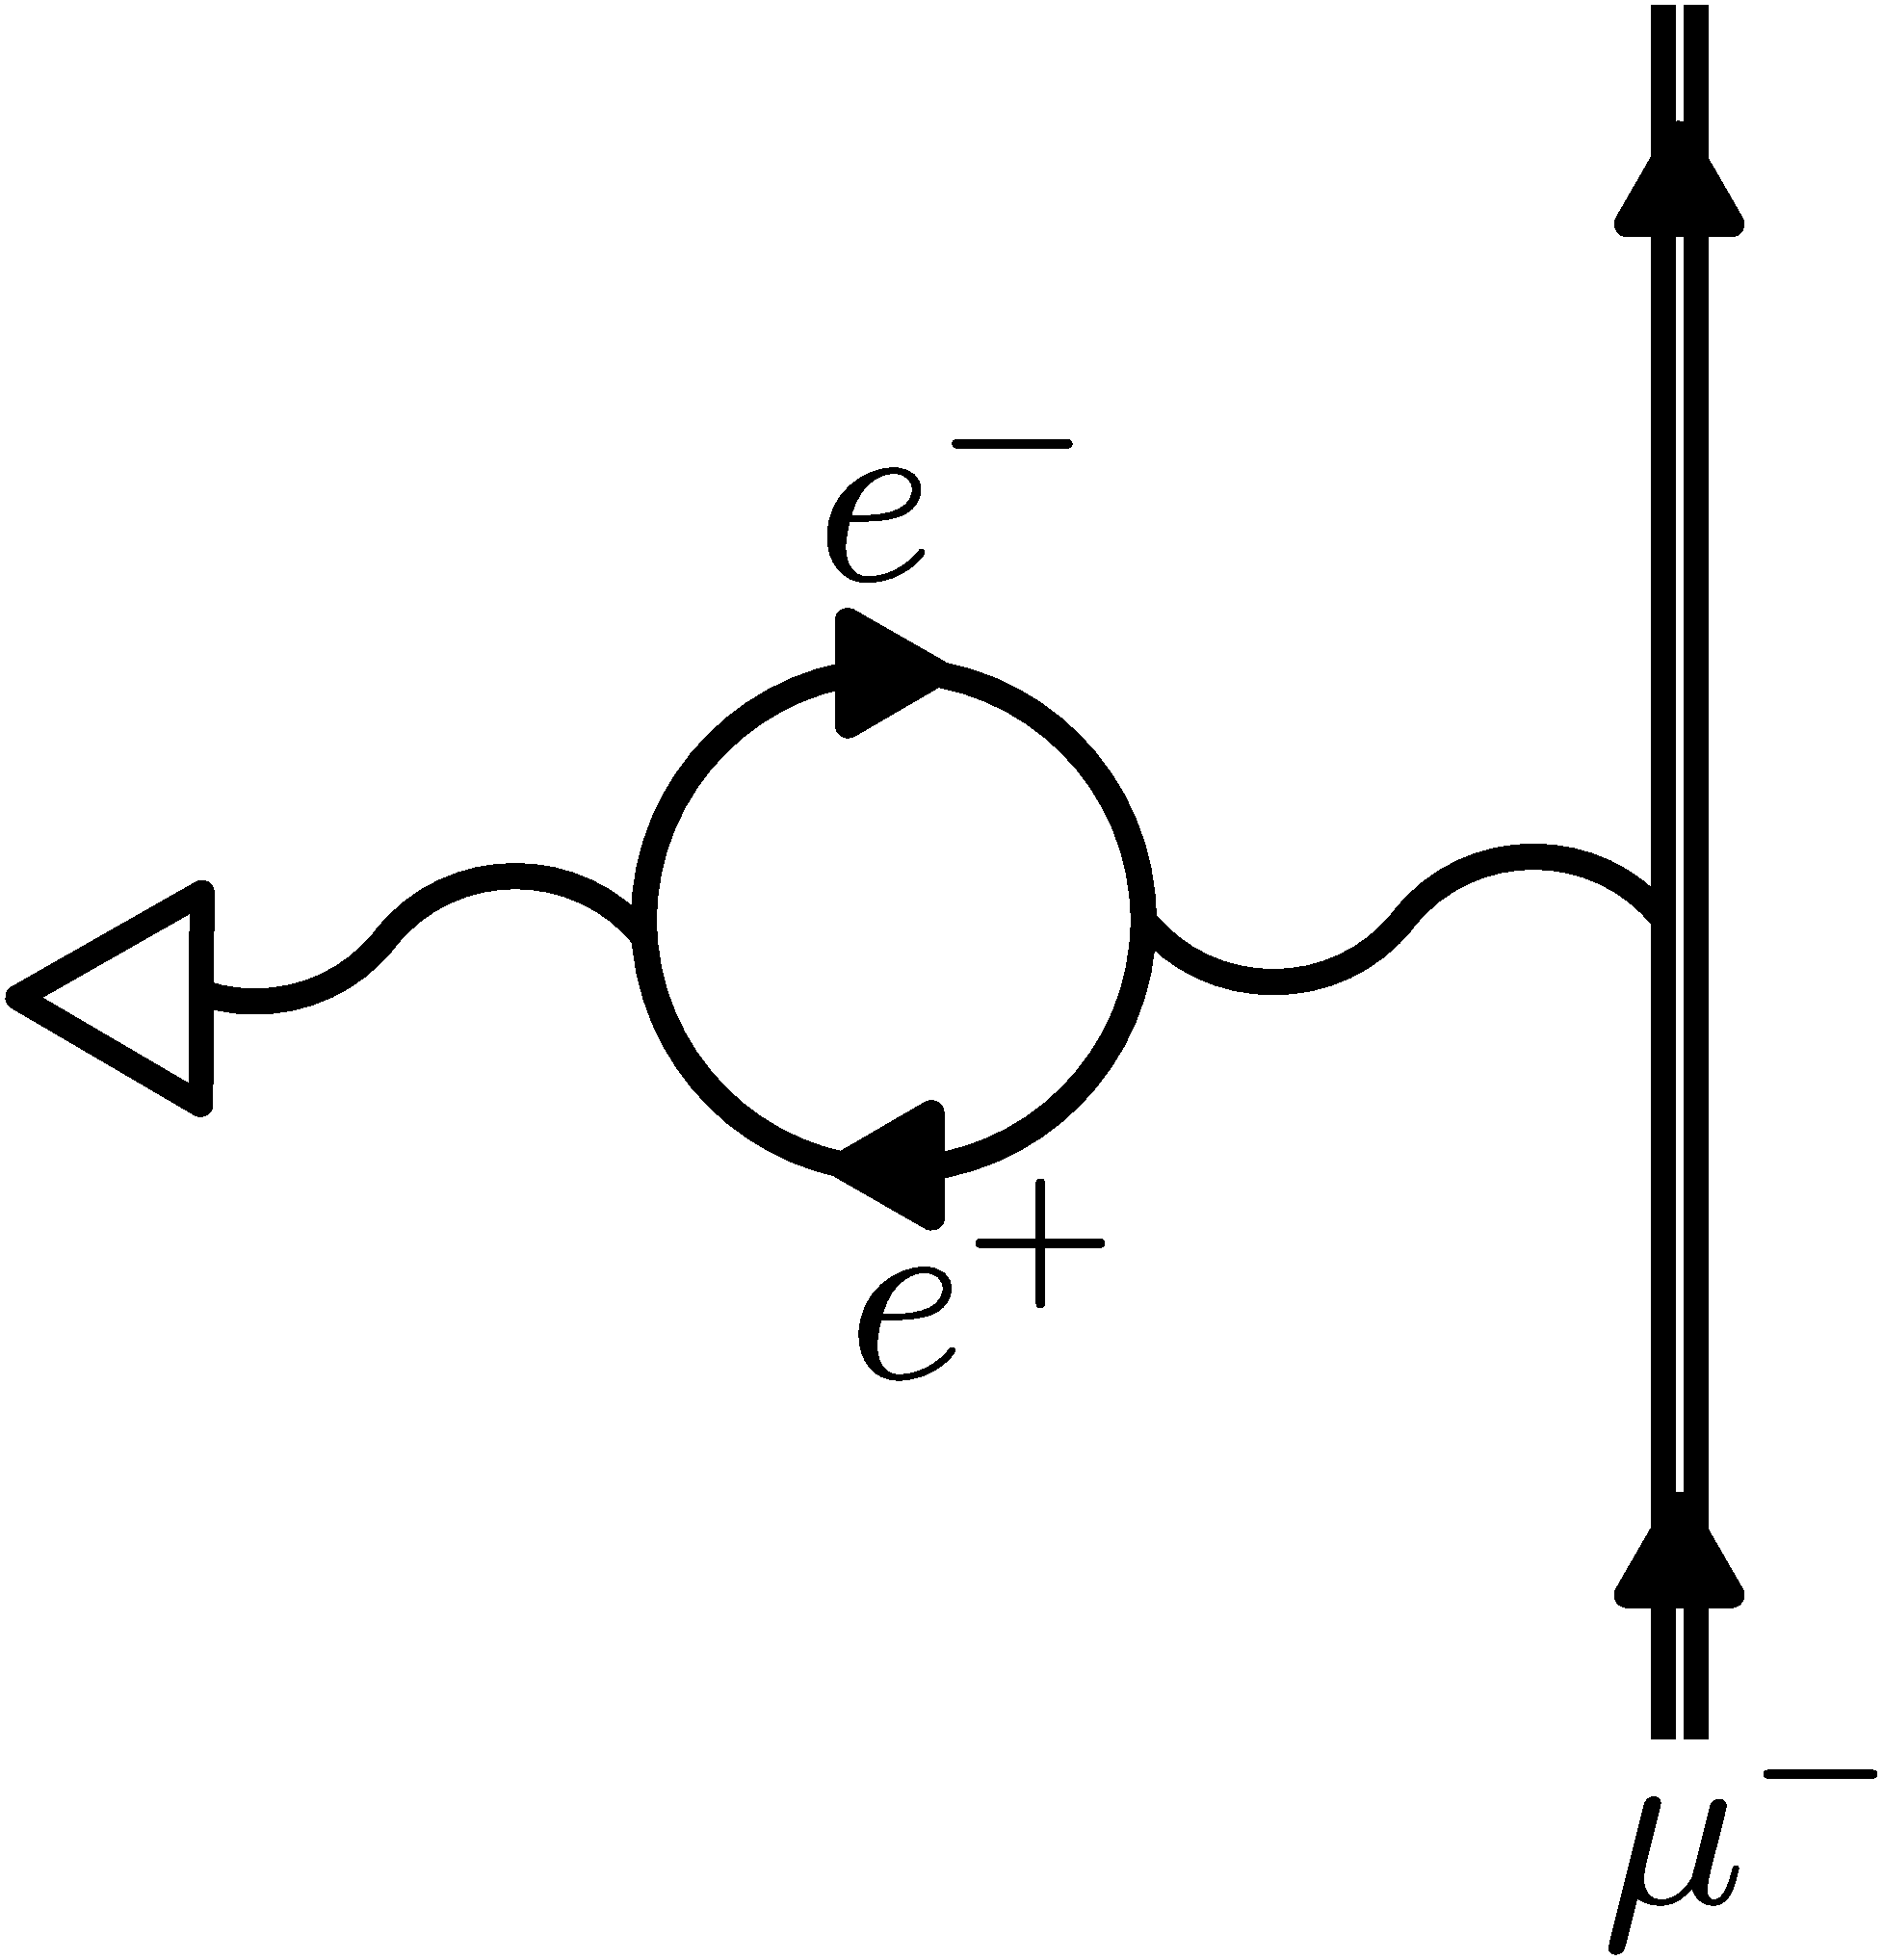
\includegraphics[width=0.30\textwidth]{pics/quehl}\\
%$\qquad\qquad\qquad\qquad$(a)\hfill(b)$\qquad\qquad\qquad\qquad$
\caption{
Feynman diagrams for the leading order contributions of the vacuum polarization to the quadrupole interaction in muonic atoms. An external double line stands for the bound-muon wave function. A single internal line for the free electron propagator, and a wave line for the photon propagator. A cross represents the interaction with the monopole potential, and a triangle the interaction with the quadrupole potential. Contribution (a) is calculated by including the spherically symmetric contribution of the Uehling potential~\eqref{eq:sph_uehl} in the Dirac equation; contribution (b) by including the quadrupole contribution of the Uehling potential~\eqref{eq:defmultiuehl} in the matrix elements.
}
\label{fig:quehl}
\end{figure}
% end quad uehl figure
%
The approach is applicable for arbitrary charge distributions, and is applied for the quadrupole term with $l=2$ in Section~\ref{sec:muon_re}. In the following, the quadrupole term $l=2$ is considered for the models of a charged-shell and point-like quadrupole distribution, where the corresponding term in Eq.~\eqref{eq:defmultiuehl} can be simplified. For the charged-shell quadrupole distribution, the nuclear charge distribution is written as
\begin{alignat}{2}
&\rho(\mathbf{r}_N)&&=\rho_0(r_N) + \rho_2(r_N,\vartheta_N)\\
&\rho_2(r_N,\vartheta_N)&&=-\alpha Q_0 \frac{5}{8\pi }\frac{\delta(r-R)}{R^4}
P_2(\cos\vartheta_N),
\end{alignat}
where the intrinsic quadrupole moment $Q_0$ is concentrated at the nuclear radius $R$. Thereby, the quadrupole part of the Uehling potential~\eqref{eq:defmultiuehl} reads
\begin{equation}
V^{(2)}_{\text{uehl}}(\mathbf{r}_\mu,\phi,\theta)=
-\alpha Q_0 \frac{\alpha}{3\pi}\frac{c_2(r_\mu,R)}{R^2}\sum\limits_{m=-l}^{l} C_{lm}^*(\theta,\phi)C_{lm}(\vartheta_\mu,\varphi_\mu).
\label{eq:quadUehlShell}
\end{equation}
A point-like quadrupole moment corresponds to the limit of zero nuclear radius $R$ in Eq.~\eqref{eq:quadUehlShell}. The limit cannot be calculated naively due to the $R^{2}$ factor in the denominator. However, it turns out that the Taylor expansion of $c_2(r_\mu,R)$ around $R=0$ has no constant and no linear term. Therefore, $c_2(r_\mu,R)$ can be expanded for small $R$ as
\begin{equation}
c_2(r_\mu,R) = \frac{K_1(2m_er_\mu)+2m_er_\mu K_2(2m_er_\mu)+4m_e^2r_\mu^2/3K_3(2m_er_\mu)}{r^3}R^2 + \mathcal{O}(R^3),
\end{equation}
and therby the point-like limit of quadrupole Uehling potential reads
\begin{alignat}{2}
\label{eq:quadUehlpoint}
&V^{(2)}_{\text{uehl}}(\mathbf{r}_\mu,\phi,\theta)&&=
-\alpha Q_0\, g(r) \sum\limits_{m=-l}^{l} C_{lm}^*(\theta,\phi)C_{lm}(\vartheta_\mu,\varphi_\mu).\\
&\qquad\qquad g(r)&&=\frac{\alpha}{3\pi}\frac{K_1(2m_er_\mu)+2m_er_\mu K_2(2m_er_\mu)+4m_e^2r_\mu^2/3K_3(2m_er_\mu)}{r^3}.
\label{eq:quadUehlShellLimit}
\end{alignat}
The expressions for the quadrupole Uehling potential for the charged-sphere and point-like distributions from Eqs.~\eqref{eq:quadUehlShell},~\eqref{eq:quadUehlpoint}, respectively, can be used for testing the implementation of the general case in Eq.~\eqref{eq:defmultiuehl}.\\


\subsection{Residual second order corrections}
\label{sec:muon_residualSO}
The rediagonalization of the hyperfine interaction in muonic atoms is explained in Section~\ref{sec:muon_dynamic}, using a modelspace consisting of a muonic fine-structure doublet and the first rotational nuclear states. Also, the leading contribution from states outside of the modelspace is derived in Eq.~\eqref{eq:pert_secondOrderEnerg}. Essentially, it is the second order energy correction due to the hyperfine interaction, excluding all states which are considered in the rediagonalization process. In the following, the residual second order corrections will be discussed for the case of the rhenium $2p$ modelspace given in Section~\ref{sec:toyModelRediag}. Here, the modelspace consists of the muonic $2p_{1/2}$ and $2p_{3/2}$ states and the nuclear $5/2,7/2,9/2$ states. This results in 18 coupled states, with values of the total angular momentum $F=1,...,6$, as shown in Fig.~\ref{fig:blockRe}. The set of these states is called $M_{\mu}$. The summation over all states, which are not in the modelspace involves all states $\left|FM_F\,I_iK_i\,n_i\kappa_i\right>$ as defined in Eq.~\eqref{eq:totalState}, where not all quantum numbers coincide with a state in the considered modelspace $M_{2p}$. In the following, this summation is schematically written as $\sum_{i\notin M_{\mu}}$.

After the subspace has been chosen and rediagonalization has been performed, the quadrupole interaction with states outside of the subspace leads to residual second order corrections to the energy levels~\cite{chen1970}.
For the total second order correction a summation/integration over the complete (discrete and continous) spectrum for both nuclear and muonic states has to be performed. For the complete nuclear spectrum, sophisticated models or numerous experimental data are required. However, the muon is point-like and can be described as a Dirac particle. Therefore, in this work, we calculate the second order corrections due to the electric quadrupole (Eq.~\eqref{eq:quadPot}) and quadrupole-Uehling interaction (${l}{=}{2}$-term in Eq.~\eqref{eq:defmultiuehl}), where the nucleus stays in the rotational ground state, but the complete muonic spectrum is considered.
For a composite state from Eq.~\eqref{eq:rediagonState}, where the hyperfine interaction is diagonalized in the modelspace, the second order energy shift due to states outside of the modelspace is
\begin{equation}
\Delta E_{\text{2.ord.}}^{(F,k)}= \sum_{i\notin M_{\mu}}\frac{\left|\left< FM_Fk\right|{V_{\text{el}}^{(2)}}{+}{V_{\text{uehl}}^{(2)}}\left|FM_Fn_i\kappa_iI_iK \right>\right|^2}{E_{F,k}-E_i},
\label{eq:second}
\end{equation}
where the sum is to be taken over all states not considered in the rediagonalization, including continuum states of the muon, and the unperturbed energy of the state $i$ is $E_i=E_{n_i\kappa_i}+E_{I_i}$.













\subsection{Evaluation for $^{185}\text{Re}$ \& $^{235}\text{U}$}
Calculations of the quadrupole-Uehling potential and the residual second order corrections have been performed for muonic rhenium and uranium, assuming a deformed Fermi nuclear charge distribution which reads as
\begin{equation}
\rho_{ca\beta}(\mathbf{r}\,)=N\left[1+\exp \left(\cfrac{r-c(1+\beta \text{Y}_{20}(\vartheta))}{a}\right)\right]^{-1},
\label{eq:deffermi_2}
\end{equation}
where $c$ is the half-density radius, $a$ the skin thickness, $\beta$ the deformation parameter, and $N$ a normalization constant determined by the condition
\begin{equation}
\int \text{d}^3r\, \rho_{ca\beta}(\mathbf{r}\,)=1.
\end{equation}
Using the deformed Fermi distribution has proved to be suitable for the description of the level structure of heavy muonic atoms, e.g.~\cite{hitlin1970,tanaka1984,tanaka1984_2}.
Values for the parameters can be estimated by using a value ${a}{=}{2.3\,\text{fm}/(4\ln 3)}$, which has proved to be a sufficiently accurate value for most nuclei~\cite{Beier2000}. Then, $c$ and $\beta$ are chosen such that the quadrupole moment and RMS value of the distribution are in agreement with the literature values from~\cite{Angeli2013,Stone2005}. For the nuclear states involved in the dynamical hyperfine structure, also the excitation energies are needed from literature~\cite{ENSDF}. The used parameters are summarized in Table~\ref{tab:params}.
With these parameters, the electric and Uehling potentials, both monopole and quadrupole parts, can be calculated numerically. The muon wave functions are obtained by solving the Dirac equation~\eqref{eq:muonicEn} with the dual-kinetic-balance method~\cite{Shabaev2004}. Thereby, a complete set of muonic bound and continuum states is obtained. An overview for the binding energies of muon states important for the dynamical hyperfine splitting are shown in Table~\ref{tab:monopole}.

The quadrupole matrix elements can be calculated both for the rediagonalization in the dynamical hyperfine structure and for the evaluation of the residual second-order terms \eqref{eq:second}, using Eq.~\eqref{eq:quadNonDiagEl}. As the next step, the total Hamiltonian~\eqref{eq:muon_htotal} is diagonalized in finite subspaces or modelspaces consisting of the muonic ($2p_{1/2}$, $2p_{3/2}$) or ($3d_{3/2}$, $3d_{5/2}$) doublet states and nuclear ground state rotational band. For rhenium, the first six states with $I =5/2,...,15/2$ are considered, and for uranium with $I =7/2,...,17/2$. The excitation energies of the nuclear states are summarized, along with other nuclear parameters, in Table~\ref{tab:params}. Thereby, the composite states and corresponding energies~$E_{\text{quad}}$ from Eq.~\eqref{eq:rediagonState} are obtained and finally, for each of these states the residual second order quadrupole correction \eqref{eq:second} is calculated. Here, the intermediate sum goes over the rotational nuclear and muonic states not included in the modelspace.
For the muonic ground state, a rediagonalization is not necessary, since the diagonal matrix elements of the quadrupole interactions vanish for muonic states with $j=1/2$.
The quadrupole-Uehling contribution to the binding energies is the difference of two calculations; once all matrix elements contain both the electric and Uehling interaction $\left({V_{\text{el}}^{(2)}}{+}{V_{\text{uehl}}^{(2)}}\right)$ and a second time only with the electric part ${V_{\text{el}}^{(2)}}$ from Eq.\eqref{eq:quadNonDiagEl}. Results for the residual second order quadrupole correction from Eq.~\eqref{eq:second} and for the quadrupole-Uehling corrections can be found in Table~\ref{tab:hfs_2} for a number of states.\\

To conclude, the improved calculation of the higher order effects, the quadrupole interaction in the framework of the dynamical hyperfine structure in heavy muonic atoms was analyzed by a fully relativistic treatment of the quadrupole-Uehling potential and of the residual second order terms.
The quadrupole-Uehling interaction was obtained rigorously by a multipole expansion of the Uehling potential for an arbitrary nuclear charge distribution.
Since it has the same angular structure as the conventional quadrupole interaction, the quadrupole-Uehling expectation value also vanishes between two muonic states with $j=1/2$, thus it does not affect the muonic ground state.
The calculations for uranium show that it can lead to energy corrections almost on the keV level for very heavy nuclei with muonic $2p$ states and thus can be potentially visible in the current experiments. Being a short-ranged potential, it falls of quickly for states further away from the nucleus. For states with $n\geq3$, we find values below $0.15\,$keV even for highest Z.
The generalization to Uehling corrections for higher-order multipoles is straight-forward. In the case of muonic atoms, since the influence of higher order multipoles is already small, this correction is expected to be negligible.
The residual second order quadrupole corrections in the dynamical hyperfine structure were calculated numerically using a basis of relativistic wave functions including the nuclear finite-size correction and monopole Uehling correction.
In contrast to the first order terms, the muonic ground state energy is affected by the second order corrections. Here, the energy correction amounts up to several keV. Also for muonic $2p$ states, it is of similar size. For the $3d$ levels, we find the energy corrections below $0.5\,$keV, both for rhenium and uranium.
If a more advanced nuclear model than the rotational model is used, the additional nuclear states appear as intermediate states in the second order corrections, leading to the nuclear polarization corrections. Therefore, the approach presented in this work provides an excellent basis for an accurate treatment of the muonic spectrum of the nuclear polarization effect in deformed muonic atoms.

%begin params table
\begin{table}[b]
\caption{\label{tab:params}%
Nuclear parameters used in the numerical calculations. $I_0$ is the nuclear ground state angular momentum. RMS and $Q_\text{spec}$ are the nuclear RMS radius and spectroscopic quadrupole moment of the nuclear ground state from~\cite{Angeli2013,Stone2005}, respectively. $c$, $a$, $\beta$ are the parameters of the deformed Fermi distribution derived from RMS and $Q_\text{spec}$. $E_{I}$ are the excitation energies of the nuclear rotational states with angular momentum $I$ (values are taken from Ref.~\cite{ENSDF}).}
%\begin{ruledtabular}
\centering
\begin{tabular}{r|ll}
& $^{185}_{\phantom{1}75}$Re & $^{235}_{\phantom{1}92}$U\\ \hline \\[-10pt]
$I_0$ \hfill$\phantom{.}$ & $5/2$ & $7/2$ \\
RMS \hfill[fm] & $5.3596(172)$ & $5.8337(41)$ \\
$Q_\text{spec}$ \hfill[b] & $2.21(4)\phantom{111}$ & $4.936(6)\phantom{1}$ \\
$c$ \hfill[fm] & $6.3517$ & $6.9562$ \\
$a$ \hfill[fm] & 0.5234 & 0.5234 \\
$\beta$ \hfill$\phantom{.abc.}$ & 0.2322 & 0.2711 \\[7pt]
$E_{I_0 + 1}$ \hfill[keV] & 125.3587(9) &  $\phantom{1}$46.108(8) \\
$E_{I_0 + 2}$ \hfill[keV] & 284.2(3) & 103.903(8) \\
$E_{I_0 + 3}$ \hfill[keV] & 475.7(4) & 171.464(13) \\
$E_{I_0 + 4}$ \hfill[keV] & 697.1(5) & 250.014(21) \\
$E_{I_0 + 5}$ \hfill[keV] & 949.7(5) & 339.976(24) \\
\end{tabular}
%\end{ruledtabular}
\end{table}
%

%begin monopole table
\begin{table}[b]
\caption{\label{tab:monopole}%
Binding energies of the low-lying, unperturbed muonic states due to the spherically symmetric parts of the electric and Uehling potential obtained by solving Eq.~\eqref{eq:muonicEn} for muonic rhenium and uranium. $E_{\rm{c}}$ shows the binding energies for a point-like Coulomb potential, $E_{\rm{fs}}$ and $E_{\rm{uehl}}$ include the finite size corrections without and with Uehling potential, respectively. All energies are in keV.
}
%\begin{ruledtabular}
\centering
\begin{tabular}{c|crrr}
& state & $E_{\rm{c}}$& $E_{\rm{fs}}$ &$E_{\rm{uehl}}$\\ \hline \\[-7pt]
$^{185}_{\phantom{m}75}$Re & $1s_{1/2}$ & 17229.12 & 9333.46 & 9394.02 \\
& $2s_{1/2}$ & 4398.85 & 3083.91 & 3100.44 \\
& $2p_{1/2}$ & 4398.85 & 4032.61 & 4059.50 \\
& $2p_{3/2}$ & 4033.07 & 3885.75 & 3910.50 \\
& $3s_{1/2}$ & 1912.97 & 1498.01 & 1504.28 \\
& $3p_{1/2}$ & 1912.97 & 1789.84 & 1798.66 \\
& $3p_{3/2}$ & 1804.01 & 1751.38 & 1759.75 \\
& $3d_{3/2}$ & 1804.01 & 1802.05 & 1810.30 \\
& $3d_{5/2}$ & 1773.14 & 1772.36 & 1780.16 \\[7pt]
$^{235}_{\phantom{1}92}$U&$1s_{1/2}$ & 27351.29 & 12100.56 & 12175.51 \\
& $2s_{1/2}$ & 7074.68 & 4308.67 & 4332.13 \\
& $2p_{1/2}$ & 7074.68 & 5901.35 & 5941.39 \\
& $2p_{3/2}$ & 6130.65 & 5674.78 & 5711.89 \\
& $3s_{1/2}$ & 3033.18 & 2148.86 & 2158.31 \\
& $3p_{1/2}$ & 3033.18 & 2645.58 & 2659.26 \\
& $3p_{3/2}$ & 2751.54 & 2588.19 & 2601.27 \\
& $3d_{3/2}$ & 2751.54 & 2739.69 & 2754.06 \\
& $3d_{5/2}$ & 2679.66 & 2674.77 & 2688.10

\end{tabular}
%\end{ruledtabular}
\end{table}
%
%begin hfs table
\begin{table*}
\begin{small}
\caption{\label{tab:hfs_2}
Overview of energy corrections due to residual second order electric quadrupole splitting~$\Delta E_{\text{2.ord.}}$ and quadrupole-Uehling interaction~$\Delta E_{\text{quad-uehl}}$ for $^{185}$Re and $^{235}$U. $F$ is the total angular momentum of muon and nucleus, $I_N$ is the nuclear angular momentum and $\mu$-state is the muonic state in spectroscopic notation. For the muonic $2p$ and $3d$ states, these are mixed by the dynamical hyperfine structure, thus $I_N$ (main) and $\mu$-state (main) denote states with the largest contribution. $E_{\text{quad}}$ is the binding energy without quadrupole Uehling and residual second order quadrupole interaction. The states are ordered descending in the total energy~$E_{\text{tot}}$. See Section~\ref{sec:higherorder} for details. All energies are in keV.}
%\begin{ruledtabular}
\centering
\begin{tabular}{l|rccccc|c}
 &F&\multicolumn{1}{c}{$I_{N}\,\text{(main)}$}&$\mu\text{-state (main)}$&\multicolumn{1}{c}{$E_{\text{quad}}$}&\multicolumn{1}{c}{$\Delta E_{\text{2.ord.}}$}&\multicolumn{1}{c}{$\Delta E_{\text{quad-uehl}}$}&\multicolumn{1}{c}{$E_{\text{tot}}$}\\\hline\\[-7pt]
$^{185}_{\phantom{1}75}\text{Re}$&  2 &   \nicefrac{5}{2} & $1s_{1/2}$& 9394.02 &  3.21 &   0.00 & 9397.23 \\
&  6 &  \nicefrac{13}{2} & $1s_{1/2}$& 8696.92 &  2.06 &   0.00 & 8698.98 \\
&  8 &  \nicefrac{15}{2} & $1s_{1/2}$& 8444.32 &  1.76 &   0.00 & 8446.08 \\
&  2 &   \nicefrac{5}{2} & $2p_{1/2}$ & 4083.31 &  2.18 &  0.28 & 4085.77 \\
&  3 &   \nicefrac{5}{2} & $2p_{1/2}$ & 4077.79 &  2.07 &  0.23 & 4080.09 \\
&  3 &   \nicefrac{9}{2} & $2p_{3/2}$ & 3992.27 &  2.41 &  0.41 & 3995.09 \\
&  4 &   \nicefrac{7}{2} & $2p_{1/2}$ & 3957.33 &  2.10 &  0.26 & 3959.69 \\
&  3 &   \nicefrac{5}{2} & $2p_{3/2}$ & 3886.35 &  1.12 & -0.22 & 3887.25 \\
&  5 &   \nicefrac{7}{2} & $2p_{3/2}$ & 3814.27 &  2.08 &  0.28 & 3816.63 \\
&  4 &   \nicefrac{9}{2} & $2p_{1/2}$ & 3734.93 &  1.03 & -0.27 & 3735.69 \\
&  6 &   \nicefrac{9}{2} & $2p_{3/2}$ & 3650.57 &  1.95 &  0.25 & 3652.77 \\
&  5 &   \nicefrac{9}{2} & $2p_{3/2}$ & 3556.36 &  1.13 & -0.24 & 3557.25 \\
&  7 &  \nicefrac{11}{2} & $2p_{3/2}$ & 3458.14 &  1.85 &  0.23 & 3460.22 \\
&  6 &  \nicefrac{11}{2} & $2p_{3/2}$ & 3344.35 &  0.93 & -0.19 & 3345.09 \\
&  8 &  \nicefrac{13}{2} & $2p_{3/2}$ & 3111.03 &  0.68 &  0.02 & 3111.73 \\
&  7 &  \nicefrac{15}{2} & $2p_{3/2}$ & 2941.66 &  0.82 & -0.15 & 2942.33 \\
&  8 &  \nicefrac{15}{2} & $2p_{3/2}$ & 2938.52 &  0.67 & -0.16 & 2939.03 \\
&  3 &   \nicefrac{5}{2} & $3d_{3/2}$ & 1815.47 &  0.07 &  0.03 & 1815.57 \\
&  1 &   \nicefrac{5}{2} & $3d_{3/2}$ & 1804.28 &  0.11 & -0.03 & 1804.36 \\
&  3 &   \nicefrac{7}{2} & $3d_{5/2}$ & 1783.72 &  0.05 &  0.02 & 1783.79 \\
&  0 &   \nicefrac{5}{2} & $3d_{5/2}$ & 1772.11 &  0.11 & -0.04 & 1772.18 \\[7pt]
$^{235}_{\phantom{1}92}\text{U}$&  3 &   \nicefrac{7}{2} & $1s_{1/2}$& 12175.51 &  6.83 &   0.00 & 12182.34 \\
&  7 &  \nicefrac{15}{2} & $1s_{1/2}$& 11925.50&  4.66 &  0.00  & 11930.16 \\
&  9 &  \nicefrac{17}{2} & $1s_{1/2}$& 11835.54&  3.54 &  0.00  & 11839.08 \\
&  3 &   \nicefrac{7}{2} & $2p_{1/2}$ & 6019.06 &  5.99 &  0.85 & 6025.90 \\
&  4 &   \nicefrac{7}{2} & $2p_{1/2}$ & 6015.01 &  5.96 &  0.83 & 6021.80 \\
&  4 &   \nicefrac{9}{2} & $2p_{1/2}$ & 5979.31 &  6.02 &  0.86 & 5986.19 \\
&  5 &   \nicefrac{9}{2} & $2p_{3/2}$ & 5928.94 &  6.06 &  0.88 & 5935.88 \\
&  6 &  \nicefrac{11}{2} & $2p_{3/2}$ & 5868.85 &  6.00 &  0.89 & 5875.74 \\
&  7 &  \nicefrac{15}{2} & $2p_{1/2}$ & 5798.66 &  5.30 &  0.91 & 5804.87 \\
&  8 &  \nicefrac{15}{2} & $2p_{1/2}$ & 5745.59 &  4.71 &  0.87 & 5751.17 \\
&  5 &   \nicefrac{7}{2} & $2p_{3/2}$ & 5673.10 &  3.12 & -0.42 & 5675.80 \\
&  6 &   \nicefrac{9}{2} & $2p_{3/2}$ & 5621.02 &  3.02 & -0.46 & 5623.58 \\
&  2 &   \nicefrac{7}{2} & $2p_{3/2}$ & 5620.12 &  2.78 & -0.56 & 5622.34 \\
&  9 &  \nicefrac{17}{2} & $2p_{1/2}$ & 5613.24 &  2.05 &  0.13 & 5615.42 \\
&  3 &   \nicefrac{9}{2} & $2p_{3/2}$ & 5586.28 &  2.81 & -0.54 & 5588.55 \\
&  7 &  \nicefrac{13}{2} & $2p_{1/2}$ & 5556.38 &  2.60 & -0.50 & 5558.48 \\
&  9 &  \nicefrac{15}{2} & $2p_{3/2}$ & 5493.59 &  2.44 &  0.24 & 5496.27 \\
&  8 &  \nicefrac{15}{2} & $2p_{1/2}$ & 5479.30 &  2.14 & -0.53 & 5480.91 \\
& 10 &  \nicefrac{17}{2} & $2p_{3/2}$ & 5393.16 &  1.77 &  0.13 & 5395.06 \\
&  9 &  \nicefrac{17}{2} & $2p_{3/2}$ & 5315.81 &  1.73 & -0.44 & 5317.10 \\
&  3 &   \nicefrac{7}{2} & $3d_{3/2}$ & 2767.16 &  0.44 &  0.09 & 2767.69 \\
&  1 &   \nicefrac{7}{2} & $3d_{5/2}$ & 2663.35 &  0.61 & -0.13 & 2663.83 \\
\end{tabular}
%\end{ruledtabular}
\end{small}
\end{table*}
% end hfs table























\cleardoublepage
\section{Structure of muonic $^{185}\text{Re}$ \& $^{187}\text{Re}$}
\label{sec:muon_re}
The analysis of x-rays emitted due to transitions in muonic atoms constitutes one possibility to obtain information on the nuclear charge distribution and measure properties like RMS charge radii, or nuclear quadrupole moments. This section analyzes the structure of muonic rhenium-185 and -187. So far, there is no absolute measurement of the charge radius of $^{185}$Re~\cite{schopper2004} and the only experiment reported on muonic rhenium is an extraction of the quadrupole moments of $^{185}$Re and $^{187}$Re from the N x-rays (${n}{=}{5}\rightarrow{n}{=}{4}$) of natural Re~\cite{konijn1979}, which is mainly a mixture of these two isotopes. Therefore, the theoretical spectra of both isotopes have been used at the same time for fitting the experimental spectrum. As a consequence, the two extracted quadrupole moments in Ref.~\cite{konijn1979} are not indepentent. During the work on this thesis, the quadrupole moments were extracted independently for these two isotopes.
The experimental data used in this section comes from measurements of muonic x-rays with isotopically pure rhenium performed in 2016 by the MuX Collaboration. The high intensity muon beam at the Paul Scherrer Institute (Switzerland)~\cite{psiExperiments,psiFacilities} was used as a muon source.

In the following, the muonic transition energies and transition probabilities are analyzed, where the methods described in Sections~\ref{sec:calculationSpectraMuon} and~\ref{sec:higherorder} are used. Thereby, the dependence of transitions and intensities of the $N$ x-rays ($n=5\rightarrow n=4$) on the quadrupole moment is used in combination with experimental data on isotopically pure $^{185}$Re and $^{187}$Re to extract the nuclear quadrupole moment. Also, a good qualitative description based on the rigid-rotor nuclear model (Appendix~\ref{app:rig_rotor}) of the $K$ x-rays ($2p\rightarrow 1s$) is given.


%\subsection{Extraction of quadrupole moment from $5g\rightarrow 4f$ transitions}
After the muon beam hits the target, a muon can be captured in the Coulomb field of an atomic nucleus in a highly excited states. Then, it starts cascading towards the ground state. In principle, this is a complicated many-body probmlem, involing the nucleus, the muon and the atomic electrons. However, there is an intermediate region with $n\approx 4 - 7$, where finite nuclear size effects are still rather small and at the same time, the muon is not influenced significantly by the surrounding atomic electrons. Therefore, the system is essentially hydrogen-like and no many-body problem has to be solved. In addition, the hyperfine structure is mainly determined by the nuclear quadrupole moment. It has been realized, that in this region, more specifically the ${n}{=}{5}\rightarrow{n}{=}{4}$ transitions, nuclear quadrupole moments can be extracted, which has been done for lutetium-175 in Ref.~\cite{Dey1979} and for natural rhenium in Ref.~\cite{konijn1979}.
As a first application of the calculation of muonic spectra presented in this thesis, the dependence of the transition energies and intensities of the muonic $N$ x-rays on the nuclear quadrupole moment is calculated, and by comparing to measurements of isotopically pure $^{185}$Re and $^{187}$Re, a value for their spectroscopic quadrupole moment is extracted.

Following Section~\ref{sec:transitions}, the most intense transitions are the $E1$-transitions in the circular orbits $5g_{9/2}\rightarrow4f_{7/2}$ and $5g_{7/2}\rightarrow4f_{7/2}$. However, also the $5f_{7/2}\rightarrow4d_{5/2}$, $5g_{7/2}\rightarrow 4f_{7/2}$, and $5f_{5/2}\rightarrow 4d_{5/2}$ transitions have to be considered, since they almost coincide in energy with the $5g\rightarrow4f$ energies around $365\,$keV. Therefore, the following approach is chosen for the theoretical prediction: The four fine-structure states of the initial states $5g_{9/2},\,5g_{7/2},\,5f_{7/2}\,,5f_{5/2}$ together with the nuclear ground state with $I=5/2$ define a first model space. Now, the formalism described in Section~\ref{sec:muon_dynamic} can be used to calculate the energies in this modelspace, including finite size effects, vacuum polarization (Uehling, Källen-Sabry, Wichmann-Kroll in point-like approximation, quadrupole-Uehling), and rediagonalization of the electric quadrupole and magnetic dipole hyperfine interaction. In this way, also contributions non-linear in the nuclear quadrupole moment are included, in contrast to~\cite{konijn1979}.
Excited nuclear states were not considered, since the quadrupole interaction in this case is small compared to the nuclear rotational states. For the $N$ x-rays, the nuclear energy splitting is around three orders of magnitude larger. Furthermore, due to the small hyperfine splitting in the ${n}{=}{4,5}$ states, the residual second order terms, as described in Section~\ref{sec:muon_residualSO}, are very small.
The same procedure is repeated for the final states with ${n}{=}{4}$, i.e. $4f_{7/2},\,4f_{5/2},\,4d_{5/2},\,4d_{3/2}$.
Then, the transition probabilities can be calculated from each initial to each final state. For this analysis, the relativistic formulas for $E1$ and $M1$ transitions from Section~\ref{sec:transitions} are used, assuming an initial statistical population $\sim (2F+1)$ for each initial state with total angular momentum $F$. Transitions of higher-order multipolarity have a much smaller transition rate. With this approach, every transition energy and corresponding intensity can be calculated for a given nuclear charge distribution
\begin{equation}
\rho_N(r_N,\vartheta_N)=N\left[1+\exp\left(\cfrac{r_N-c(1+\beta \text{Y}_{20}(\vartheta_N))}{a}\right)\right]^{-1},
\end{equation}
where $N$ is a normalization constant fixed by the condition $\int\text{d}^3\mathbf{r} \rho(r,\vartheta) = Z$.
The three parameters $a$, $c$, $\beta$ are calculated using $a=2.3\,\text{fm}/(4\ln3)$, which is a reasonable estimate for most nuclei~\cite{Beier2000}, such that the RMS charge radius agrees with the literature value from Ref.~\cite{Angeli2013}, and the spectroscopic quadrupole moment with some given value~$Q$. The connection of the spectroscopic quadrupole~$Q$ moment with the nuclear charge distribution for a nucleus with ground state angular momentum~$I$ is
\begin{equation}
Q = 4\pi\frac{I(2I-1)}{(I+1)(2I+3)}\int\limits_0^\infty\text{d}r_N \int\limits_0^\pi\text{d}\vartheta_N\,
r_N^4 \sin\vartheta_N \rho_N(r_N,\vartheta_N)\text{P}_2(\cos\vartheta_N),
\end{equation}
where $\text{P}_l(x)$ are the Legendre polynomials from Appendix~\ref{app:special_func}.
The value of the magnetic moment needed for the calculation of the magnetic dipole interaction is taken from~\cite{STONE2016}. The influence of finite size effects was checked by also using charged shell and homogeneously charged sphere distribution.
With this parametrization, the entire spectrum can be calculated for a given spectroscopic quadrupole moment and by fitting the theoretically calculated spectrum to the experimentally measured one, the quadrupole moment can be extracted. There are five groups of $E1$-transitions in energy range of the $5g\rightarrow 4f$ transitions, namely:
\begin{enumerate}
\label{en:groups}
\item $5g_{9/2}\rightarrow 4f_{7/2}$
\item $5g_{7/2}\rightarrow 4f_{5/2}$
\item $5f_{7/2}\rightarrow 4d_{5/2}$
\item $5g_{7/2}\rightarrow 4f_{7/2}$
\item $5f_{5/2}\rightarrow 4d_{5/2}$
\end{enumerate}
Each of those groups consists of 15 or 16 individual lines itself due to the hyperfine structure. Therefore, 77 individual lines and corresponding intensities are taken into account in the fitting process.

The difference between two transition energies is especially sensitive to the quadrupole moment, since the majority of the uncertainty due to the nuclear RMS radius cancels, as described in Ref.~\cite{konijn1979}. Therefore, the energy differences of all $5g_{9/2}\rightarrow4f_{7/2}$ transition compared to the most intense transition in this group, called the centroid transition, is calculated and analogously the corresponding intensities are given relative to the centroid transition.
The same holds for the other four groups. Then, the energy difference of the $5g_{9/2}\rightarrow4f_{7/2}$ centroid compared to the other four centroids is calculated.
Thereby, the energy differences of all considered transitions compared to the $5g_{9/2}\rightarrow4f_{7/2}$ centroid is parametrized in terms of the nuclear quadrupole moment, and the position of the $5g_{9/2}\rightarrow4f_{7/2}$ centroid can be fitted to the experimental spectrum as a free parameter. The relative intensities of the 5 different groups are either free fit parameters or obtained from other programs for cascade calculations~\cite{elisa_privcomm}.
Since it is too expensive to perform full calculations in the fitting process to experimental data, the full calculations are performed for several values of the quadrupole moment in the proximity of the expected value and are fitted by a quadratic function for every transition energy and intensity as
\begin{alignat}{2}
&\Delta E^{if}(Q)&&= \Delta E^{if}_0 +  \Delta E^{if}_1 Q+  \Delta E^{if}_2 Q^2,\label{eq:en_fit}\\
&\phantom{\Delta}I^{if}(Q)&&= I^{if}_0 +  I^{if}_1 Q+  I^{if}_2 Q^2.\label{eq:tran_fit}
\end{alignat}
The fitted function and the results from the full calculations agree on the $10^{-4}\,$eV level in the region of the determined quadrupole moment. The resulting dependencies for $^{185}\rm{Re}$ are given in Table~\ref{tab:re185energ} for the relative transition energies, in Table~\ref{tab:re185intens} for the intensities, and in Table~\ref{tab:re185centroid} for fitted energy differences of the centroid transitions. For $^{187}$Re, the coefficients differ only to a small extent due to different values for the magnetic moment and RMS charge radius and the corresponding tables are given in Appendix~\ref{app:re187}. 
A main experimental challenge is understanding of the line shape due to the detector response function, which broadens the Lorentzian (due to natural life time) essentially into a Voigt profile. This issue is treated in Ref.~\cite{vogiatzi2018} in detail.

The calculated spectrum parametrized by the nuclear quadrupole moment can now be fitted efficiently to the experimental spectrum and the result is shown in Fig.~\ref{fig:re54}. The $5f_{5/2}\rightarrow 4d_{5/2}$ group turned out not to be visible in the fit. Thereby, the preliminary extracted spectroscopic quadrupole moment of $^{185}$Re and $^{187}$Re is obtained as
\begin{align}
Q_{\text{Re-}185} &= 2.11(2)(7)\,\text{barn},\\
Q_{\text{Re-}187} &= 1.96(2)(2)\,\text{barn},
\end{align}
where the number in the first bracket is the statistical uncertainty and the number in the second bracket is the systematic uncertainty due to the ratio of the intensities. The value is in agreement with the previous literature values~\cite{Stone2005}.%

Furthermore, the low-lying $2p\rightarrow1s$ transitions, or $K$ x-rays, have been measured during the same experiments. The assumption of statistically populated $5g$ states, i.e. $\sim (2F+1)$, and a cascade $5g\rightarrow 4f \rightarrow 3d \rightarrow 2p \rightarrow 1s$ as discussed in Sections~\ref{sec:muon_dynamic} and \ref{sec:transitions} can explain the spectrum qualitatively, using the rigid rotor model for the nucleus (Appendix~\ref{app:rig_rotor}). The corresponding comparison for the $K$ x-rays ($2p\rightarrow 1s$) is shown in Fig.~\ref{fig:re54_K}. For the calculations of the spectra, the first five nuclear rotational states have been considered. In principle, from these spectra, the nuclear RMS radius can be extracted~\cite{hitlin1970}. However, for the low-lying transitions in heavy muonic atoms, the nuclear polarization corrections, e.g.~\cite{chen1970}, have to be included into the theoretical predictions. These corrections are due to virtual excitations of nuclear states beyond the rigid rotor model and have to be treated with a more accurate nuclear model or experimental data on nuclear transitions. Thus, updated calculations from the nuclear physics side would be highly desirable together with the calculations for the bound muon as presented in this thesis in connection with the new experimental campaign on muonic atoms. 
This is also discussed in more detail in the conclusion \& outlook chapter.%
%
%re185 5-4 figure
\begin{figure}%
\centering
\subfloat[]{\label{fig:comp54exp}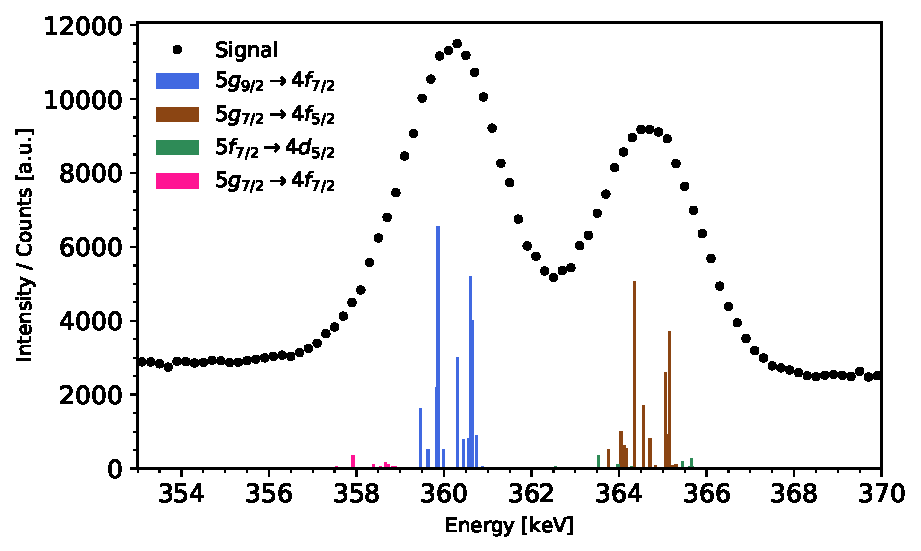
\includegraphics[width=0.95\linewidth]{pics/comparison_54}}\\
\subfloat[]{\label{fig:comp54theo}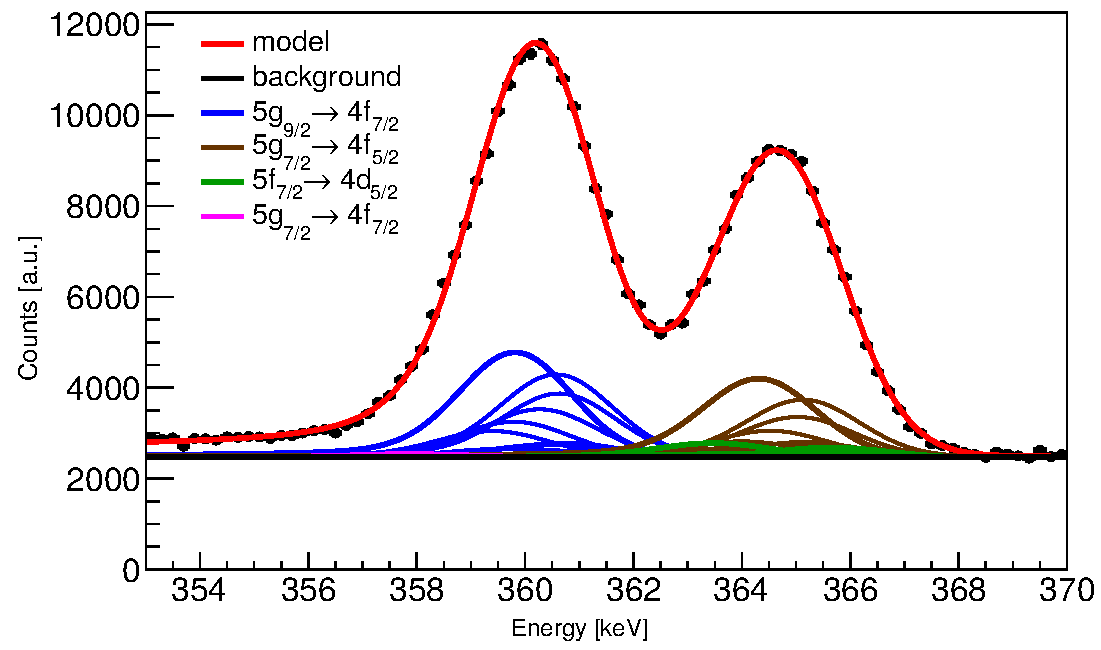
\includegraphics[width=0.915\linewidth]{pics/comparison_exp}}
\caption{
Comparison of the experimental data and theoretical predictions in region of the $5g_{9/2}\rightarrow4f_{7/2}$, $5g_{7/2}\rightarrow4f_{7/2}$, $5f_{7/2}\rightarrow4d_{5/2}$, $5g_{7/2}\rightarrow4f_{7/2}$ groups in $^{185}$Re. The black dots are the measurements and the nuclear quadrupole moment of $^{185}$Re has been extracted by fitting the theoretical prediction to the data. 
In part (a), the colored lines show the calculated transition energies and corresponding transition probabilities.
In part (b), the predicted signals for each transition are shown. The center corresponds to the calculated transition probability and the shape is given by the natural line width and the detector response function. The red function represents the calculated total signal and is the sum of all separate signals. Details about the calculations can be found in Section~\ref{sec:muon_re}, and about the detector response function in Ref.~\cite{vogiatzi2018}.
}
\label{fig:re54}
\end{figure}%
%
% figure k x-rays
\begin{figure}%
\centering
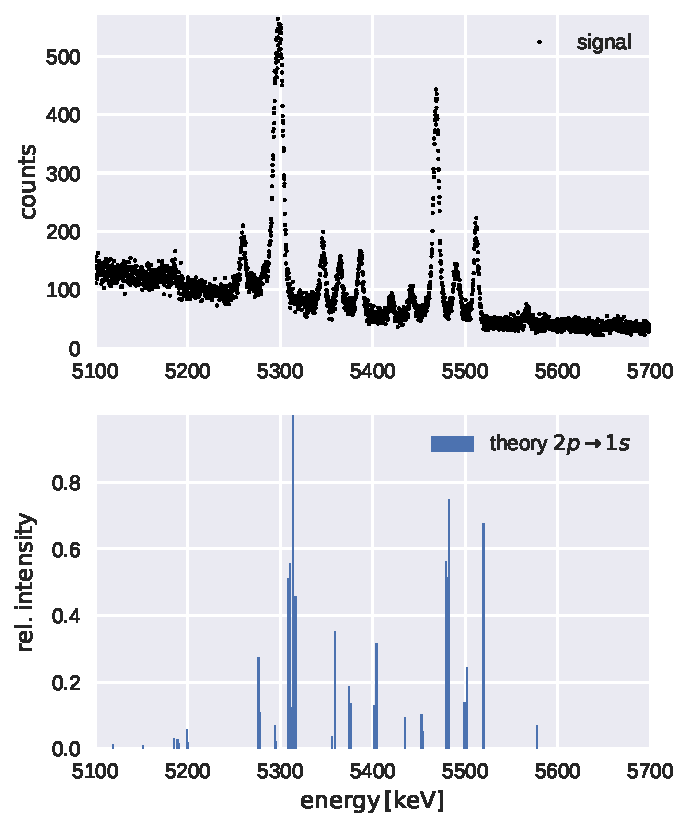
\includegraphics[width=0.99\textwidth]{pics/comparison_21}
\caption{
Comparison of experimental spectrum (upper plot) and theoretical calculations (lower plot) in the area of the $K$ x-rays for muonic $^{185}$Re. The first 5 rotational states of the $^{185}$Re nucleus and a muonic cascade starting from statistically populated $5g$ states have been used for the calculations. The spectrum is complex due to excited nuclear states and large hyperfine splitting in the muonic $2p$ states. The small shift of the theoretical values is due to the non-calculated nuclear polarization corrections. For further details, see Section~\ref{sec:muon_re}.
}
\label{fig:re54_K}
\end{figure}%
%
%
%re185 tables
%
\clearpage
\begin{table}
%\setlength\extrarowheight{1pt}
\caption{\label{tab:re185centroid}%
Quadratic fits of the energies of the centroid transitions for $^{185}$Re. The formula for the energy difference in terms of a give quadrupole moment $Q$ is given in Eq.~\eqref{eq:en_fit}. See Section~\ref{sec:muon_re} for details.}
%\begin{ruledtabular}
\centering
\begin{small}
\begin{tabular}{cc|ccc}
centroid& $F_i \rightarrow F_f$ & $\Delta E_2^{if} [\text{keV/barn}^2]$ & $\Delta E_1^{if} [\text{keV/barn}]$ & $\Delta E_0^{if} [\text{keV}]$\\[1pt]\hline%\\[1pt]
$5g_{9/2} \rightarrow 4f_{7/2}$ & $7 \rightarrow 6$ & 0.0000 & -0.1743 & 360.2145\\
$5g_{7/2} \rightarrow 4f_{5/2}$ & $6 \rightarrow 5$ & 0.0040 & -0.1601 & 364.6631\\
$5f_{7/2} \rightarrow 4d_{5/2}$ & $6 \rightarrow 5$ &-0.0016 & -0.4396 & 364.4165\\
$5g_{7/2} \rightarrow 4f_{7/2}$ & $6 \rightarrow 6$ &-0.0004 & -0.1775 & 358.2798\\
$5f_{5/2} \rightarrow 4d_{5/2}$ & $5 \rightarrow 5$ &-0.0039 & -0.4480 & 361.1407
\end{tabular}
%\end{ruledtabular}
\end{small}
\end{table}%
%\clearpage
%
%
\begin{longtable}{c c | r r r}
%\setlength\extrarowheight{1pt}
\caption{\label{tab:re185energ}%
Quadratic fits of the transitions energies compared to the most intense (centroid) transition for the 15 most intense transitions for the $5g_{9/2}\rightarrow4f_{7/2}$, $5g_{7/2}\rightarrow4f_{7/2}$, $5f_{7/2}\rightarrow4d_{5/2}$, $5g_{7/2}\rightarrow4f_{7/2}$, and $5f_{5/2}\rightarrow4d_{5/2}$ groups in $^{185}$Re. The absolute transition energies of the centroid transitions are given in Table~\ref{tab:re185centroid}. The formula for the transition energy in terms of a give quadrupole moment $Q$ is given in Eq.~\eqref{eq:en_fit}. See Section~\ref{sec:muon_re} for details.}\\
\\\hline\\[-10pt]\hline\\[-10pt]
\centering
Group& $F_i \rightarrow F_f$ & $\Delta E_2^{if} [\text{eV/barn}^2]$ & $\Delta E_1^{if} [\text{eV/barn}]$ & $\Delta E_0^{if} [\text{eV}]$\\[1pt]\hline
\endfirsthead

Group& $F_i \rightarrow F_f$ & $\Delta E_2^{if} [\text{eV/barn}^2]$ & $\Delta E_1^{if} [\text{eV/barn}]$ & $\Delta E_0^{if} [\text{eV}]$\\[1pt]\hline
\multicolumn{5}{c}{{(continuation from previous page)}}\\
\endhead

\multicolumn{5}{c}{{(continued on next page)}}\\ \endfoot
\hline \\[-10pt] \hline \endlastfoot

$5g_{9/2} \rightarrow 4f_{7/2}$ & $7 \rightarrow 6$ & 0.0000 & 0.0000 & 0.0000 \\
& $6 \rightarrow 6$ & 0.4349 & -112.8421 & -4.3710 \\
& $6 \rightarrow 5$ & -3.9990 & 374.5405 & 8.1664 \\
& $5 \rightarrow 6$ & 0.0083 & -130.4566 & -8.6014 \\
& $5 \rightarrow 5$ & -4.4255 & 356.9260 & 3.9360 \\
& $5 \rightarrow 4$ & -0.0011 & 385.3921 & 20.3954 \\
& $4 \rightarrow 5$ & -4.3353 & 397.2028 & 0.5956 \\
& $4 \rightarrow 4$ & 0.0891 & 425.6690 & 17.0550 \\
& $4 \rightarrow 3$ & -1.3357 & 210.0265 & 28.0955 \\
& $3 \rightarrow 4$ & 0.2441 & 494.0067 & 14.3378 \\
& $3 \rightarrow 3$ & -1.1807 & 278.3642 & 25.3784 \\
& $3 \rightarrow 2$ & -2.3757 & -23.6926 & 33.7363 \\
& $2 \rightarrow 3$ & -1.2154 & 350.5410 & 23.3930 \\
& $2 \rightarrow 2$ & -2.4104 & 48.4842 & 31.7510 \\
& $2 \rightarrow 1$ & -1.5016 & -218.4484 & 36.5602 \\[7pt]
$5g_{7/2} \rightarrow 4f_{5/2}$ & $6 \rightarrow 5$ & 0.0000 & 0.0000 & 0.0000 \\
& $5 \rightarrow 5$ & 0.4268 & -116.6524 & -6.0881 \\
& $5 \rightarrow 4$ & -4.0133 & 397.3030 & 15.1612 \\
& $4 \rightarrow 5$ & 0.3365 & -124.8666 & -11.3476 \\
& $4 \rightarrow 4$ & -4.1035 & 389.0888 & 9.9017 \\
& $4 \rightarrow 3$ & -2.6732 & 339.4603 & 29.0257 \\
& $3 \rightarrow 4$ & -4.2588 & 440.6240 & 5.7383 \\
& $3 \rightarrow 3$ & -2.8284 & 390.9955 & 24.8623 \\
& $3 \rightarrow 2$ & -1.6187 & 86.2278 & 39.1264 \\
& $2 \rightarrow 3$ & -2.7939 & 463.6869 & 21.6868 \\
& $2 \rightarrow 2$ & -1.5843 & 158.9191 & 35.9509 \\
& $2 \rightarrow 1$ & -2.4783 & -172.9226 & 46.2225 \\
& $1 \rightarrow 2$ & -1.3654 & 223.6477 & 33.7757 \\
& $1 \rightarrow 1$ & -2.2595 & -108.1940 & 44.0473 \\
& $1 \rightarrow 0$ & -3.9788 & -312.5737 & 49.2916 \\[7pt]
$5f_{7/2} \rightarrow 4d_{5/2}$ & $6 \rightarrow 5$ & 0.0000 & 0.0000 & 0.0000 \\
& $5 \rightarrow 5$ & 2.3569 & -252.5291 & -6.3945 \\
& $5 \rightarrow 4$ & -39.2156 & 1142.4006 & -7.6361 \\
& $4 \rightarrow 5$ & 0.0075 & -267.1910 & -14.9468 \\
& $4 \rightarrow 4$ & -41.5650 & 1127.7387 & -16.1884 \\
& $4 \rightarrow 3$ & -2.9973 & 940.7303 & 47.5074 \\
& $3 \rightarrow 4$ & -40.8162 & 1239.4485 & -21.8866 \\
& $3 \rightarrow 3$ & -2.2485 & 1052.4401 & 41.8091 \\
& $3 \rightarrow 2$ & -21.1329 & 231.4531 & 70.3569 \\
& $2 \rightarrow 3$ & -1.6192 & 1208.9013 & 37.4969 \\
& $2 \rightarrow 2$ & -20.5036 & 387.9143 & 66.0447 \\
& $2 \rightarrow 1$ & -23.4328 & -470.1437 & 68.4933 \\
& $1 \rightarrow 2$ & -20.9818 & 526.1606 & 63.5780 \\
& $1 \rightarrow 1$ & -23.9109 & -331.8974 & 66.0266 \\
& $1 \rightarrow 0$ & 1.6436 & -869.1530 & 73.0235 \\[7pt]
$5g_{7/2} \rightarrow 4f_{7/2}$ & $6 \rightarrow 6$ & 0.0000 & 0.0000 & 0.0000 \\
& $6 \rightarrow 5$ & -4.4339 & 487.3826 & 12.5375 \\
& $5 \rightarrow 6$ & 0.4268 & -116.6524 & -6.0881 \\
& $5 \rightarrow 5$ & -4.0071 & 370.7302 & 6.4493 \\
& $5 \rightarrow 4$ & 0.4173 & 399.1963 & 22.9087 \\
& $4 \rightarrow 5$ & -4.0974 & 362.5159 & 1.1898 \\
& $4 \rightarrow 4$ & 0.3270 & 390.9821 & 17.6492 \\
& $4 \rightarrow 3$ & -1.0978 & 175.3397 & 28.6898 \\
& $3 \rightarrow 4$ & 0.1718 & 442.5174 & 13.4858 \\
& $3 \rightarrow 3$ & -1.2530 & 226.8749 & 24.5264 \\
& $3 \rightarrow 2$ & -2.4480 & -75.1819 & 32.8844 \\
& $2 \rightarrow 3$ & -1.2185 & 299.5663 & 21.3508 \\
& $2 \rightarrow 2$ & -2.4135 & -2.4905 & 29.7088 \\
& $2 \rightarrow 1$ & -1.5047 & -269.4231 & 34.5180 \\
& $1 \rightarrow 2$ & -2.1947 & 62.2380 & 27.5336 \\
& $1 \rightarrow 1$ & -1.2858 & -204.6945 & 32.3428 \\[7pt]
$5f_{5/2} \rightarrow 4d_{5/2}$ & $5 \rightarrow 5$ & 0.0000 & 0.0000 & 0.0000 \\
& $5 \rightarrow 4$ & -41.5725 & 1394.9297 & -1.2415 \\
& $4 \rightarrow 5$ & 2.3621 & -267.5452 & -10.8732 \\
& $4 \rightarrow 4$ & -39.2104 & 1127.3845 & -12.1147 \\
& $4 \rightarrow 3$ & -0.6427 & 940.3761 & 51.5811 \\
& $3 \rightarrow 4$ & -39.9636 & 1153.2006 & -21.9500 \\
& $3 \rightarrow 3$ & -1.3959 & 966.1922 & 41.7458 \\
& $3 \rightarrow 2$ & -20.2803 & 145.2052 & 70.2936 \\
& $2 \rightarrow 3$ & -2.0370 & 1124.7959 & 34.4113 \\
& $2 \rightarrow 2$ & -20.9214 & 303.8089 & 62.9591 \\
& $2 \rightarrow 1$ & -23.8506 & -554.2491 & 65.4077 \\
& $1 \rightarrow 2$ & -20.4551 & 476.5200 & 57.6634 \\
& $1 \rightarrow 1$ & -23.3843 & -381.5380 & 60.1120 \\
& $1 \rightarrow 0$ & 2.1702 & -918.7936 & 67.1089 \\
& $0 \rightarrow 1$ & -22.4779 & -275.1695 & 57.4097
\end{longtable}%
%
%
%
\begin{longtable}{cc|rrr}
\caption{\label{tab:re185intens}%
Quadratic fits of the relative intensities for the 15 most intense transitions each for the $5g_{9/2}\rightarrow4f_{7/2}$, $5g_{7/2}\rightarrow4f_{7/2}$, $5f_{7/2}\rightarrow4d_{5/2}$, $5g_{7/2}\rightarrow4f_{7/2}$, and $5f_{5/2}\rightarrow4d_{5/2}$ groups in $^{185}$Re. The intensities are given relative to the most intense (cenroid) transition. The formula for the transition energy in terms of a give quadrupole moment $Q$ is given in Eq.~\eqref{eq:tran_fit}. See Section~\ref{sec:muon_re} for details.}\\
\hline\\[-10pt]\hline\\[-10pt]
\centering
Group& $F_i \rightarrow F_f$ & $I_2^{if} [\%\text{/barn}^2]$ & $I_1^{if} [\%\text{/barn}]$ & $I_0^{if} [\%]$\\[1pt]\hline\endfirsthead

Group& $F_i \rightarrow F_f$ & $I_2^{if} [\%\text{/barn}^2]$ & $I_1^{if} [\%\text{/barn}]$ & $I_0^{if} [\%]$\\[1pt]\hline
\multicolumn{5}{c}{{(continuation from previous page)}}\\
\endhead

\multicolumn{5}{c}{{(continued on next page)}}\\ \endfoot
\hline \\[-10pt] \hline
\endlastfoot
$5g_{9/2} \rightarrow 4f_{7/2}$  &  $7 \rightarrow 6$  &  0.000  &  0.000  &  100.000\\
&  $6 \rightarrow 6$  &  -0.011  &  -0.115  &  8.045\\
&  $6 \rightarrow 5$  &  -0.008  &  0.383  &  78.602\\
&  $5 \rightarrow 6$  &  0.000  &  -0.002  &  0.311\\
&  $5 \rightarrow 5$  &  -0.012  &  0.036  &  12.375\\
&  $5 \rightarrow 4$  &  0.000  &  0.214  &  60.644\\
&  $4 \rightarrow 5$  &  -0.001  &  0.012  &  0.669\\
&  $4 \rightarrow 4$  &  -0.001  &  0.109  &  13.527\\
&  $4 \rightarrow 3$  &  -0.002  &  0.007  &  45.818\\
&  $3 \rightarrow 4$  &  0.000  &  0.019  &  0.837\\
&  $3 \rightarrow 3$  &  -0.001  &  0.104  &  11.900\\
&  $3 \rightarrow 2$  &  -0.002  &  -0.102  &  33.944\\
&  $2 \rightarrow 3$  &  0.000  &  0.013  &  0.619\\
&  $2 \rightarrow 2$  &  -0.001  &  0.050  &  7.725\\
&  $2 \rightarrow 1$  &  -0.001  &  -0.105  &  25.000\\[7pt]

$5g_{7/2} \rightarrow 4f_{5/2}$  &  $6 \rightarrow 5$  &  0.000  &  0.000  &  100.000\\
&  $5 \rightarrow 5$  &  0.022  &  0.218  &  12.062\\
&  $5 \rightarrow 4$  &  0.036  &  0.360  &  72.591\\
&  $4 \rightarrow 5$  &  0.003  &  0.024  &  0.730\\
&  $4 \rightarrow 4$  &  0.008  &  0.088  &  18.102\\
&  $4 \rightarrow 3$  &  0.021  &  0.397  &  50.423\\
&  $3 \rightarrow 4$  &  0.001  &  0.009  &  1.642\\
&  $3 \rightarrow 3$  &  0.012  &  -0.046  &  19.212\\
&  $3 \rightarrow 2$  &  0.013  &  0.257  &  33.003\\
&  $2 \rightarrow 3$  &  0.002  &  -0.022  &  2.192\\
&  $2 \rightarrow 2$  &  0.009  &  -0.097  &  16.477\\
&  $2 \rightarrow 1$  &  0.009  &  0.094  &  19.797\\
&  $1 \rightarrow 2$  &  0.001  &  -0.027  &  1.829\\
&  $1 \rightarrow 1$  &  0.004  &  -0.078  &  10.989\\
&  $1 \rightarrow 0$  &  0.005  &  -0.008  &  10.262\\[7pt]

$5f_{7/2} \rightarrow 4d_{5/2}$  &  $6 \rightarrow 5$  &  0.000  &  0.000  &  100.000\\
&  $5 \rightarrow 5$  &  -0.041  &  -0.307  &  12.106\\
&  $5 \rightarrow 4$  &  -0.106  &  1.215  &  72.304\\
&  $4 \rightarrow 5$  &  0.000  &  -0.002  &  0.738\\
&  $4 \rightarrow 4$  &  -0.106  &  0.343  &  18.040\\
&  $4 \rightarrow 3$  &  -0.007  &  0.381  &  50.338\\
&  $3 \rightarrow 4$  &  -0.016  &  0.086  &  1.639\\
&  $3 \rightarrow 3$  &  -0.002  &  0.330  &  19.267\\
&  $3 \rightarrow 2$  &  -0.019  &  -0.188  &  32.976\\
&  $2 \rightarrow 3$  &  -0.001  &  0.097  &  2.206\\
&  $2 \rightarrow 2$  &  -0.009  &  0.170  &  16.510\\
&  $2 \rightarrow 1$  &  -0.018  &  -0.275  &  19.773\\
&  $1 \rightarrow 2$  &  0.000  &  0.056  &  1.836\\
&  $1 \rightarrow 1$  &  -0.010  &  0.009  &  10.995\\
&  $1 \rightarrow 0$  &  0.000  &  -0.157  &  10.257\\[7pt]

$5g_{7/2} \rightarrow 4f_{7/2}$  &  $6 \rightarrow 6$  &  0.000  &  0.000  &  100.000\\
&  $6 \rightarrow 5$  &  0.722  &  1.664  &  10.899\\
&  $5 \rightarrow 6$  &  -0.010  &  -0.401  &  10.234\\
&  $5 \rightarrow 5$  &  -0.117  &  -8.661  &  68.235\\
&  $5 \rightarrow 4$  &  0.022  &  -1.370  &  15.636\\
&  $4 \rightarrow 5$  &  -0.009  &  -1.686  &  15.656\\
&  $4 \rightarrow 4$  &  0.101  &  -3.994  &  44.693\\
&  $4 \rightarrow 3$  &  0.210  &  -3.201  &  16.754\\
&  $3 \rightarrow 4$  &  0.019  &  -1.220  &  16.889\\
&  $3 \rightarrow 3$  &  -0.120  &  0.243  &  28.837\\
&  $3 \rightarrow 2$  &  0.149  &  -2.527  &  14.555\\
&  $2 \rightarrow 3$  &  -0.054  &  0.005  &  14.624\\
&  $2 \rightarrow 2$  &  -0.166  &  1.893  &  19.289\\
&  $2 \rightarrow 1$  &  0.015  &  -0.887  &  9.296\\
&  $1 \rightarrow 2$  &  -0.066  &  0.637  &  9.265\\
&  $1 \rightarrow 1$  &  -0.128  &  1.955  &  16.650\\[7pt]

$5f_{5/2} \rightarrow 4d_{5/2}$  &  $5 \rightarrow 5$  &  0.000  &  0.000  &  100.000\\
&  $5 \rightarrow 4$  &  1.842  &  3.914  &  17.965\\
&  $4 \rightarrow 5$  &  -0.008  &  -1.155  &  16.736\\
&  $4 \rightarrow 4$  &  0.792  &  -16.181  &  56.816\\
&  $4 \rightarrow 3$  &  0.382  &  -5.451  &  24.306\\
&  $3 \rightarrow 4$  &  0.130  &  -5.071  &  24.769\\
&  $3 \rightarrow 3$  &  -0.002  &  -1.881  &  25.862\\
&  $3 \rightarrow 2$  &  0.644  &  -7.174  &  24.558\\
&  $2 \rightarrow 3$  &  -0.017  &  -1.687  &  24.986\\
&  $2 \rightarrow 2$  &  -0.278  &  3.084  &  8.988\\
&  $2 \rightarrow 1$  &  0.079  &  -3.215  &  20.127\\
&  $1 \rightarrow 2$  &  -0.351  &  2.589  &  19.702\\
&  $1 \rightarrow 1$  &  0.043  &  1.509  &  1.602\\
&  $1 \rightarrow 0$  &  -0.122  &  0.943  &  10.821\\
&  $0 \rightarrow 1$  &  -0.154  &  3.105  &  10.510
\end{longtable}
\clearpage
\section{Conclusion}
\label{sec:muon_summary}
In this chapter, the following results have been presented:\\
\begin{itemize}
\setlength{\itemsep}{0.75cm}
\item An state-of-the-art numerical approach, namely the dual-kinetic-balance method based on B-splines, has been used for fully relativistic precision calculations in muonic atoms. Many important contributions have been implemented, like finite nuclear size effects, magnetic and electric hyperfine interactions, electron screening, and the most important QED corrections. 

\item The calculations include the level mixing of low-lying nuclear rotational states and muonic fine-structure components due to strong electric quadrupole interaction. The transition energies and probabilities were calculated in this framework in a fully relativistic approach, which enables an accurate theoretical prediction of the observed spectra of heavy muonic atoms.
%This work has been published in Ref.~\cite{michel2017}.
\item Additionally, enhanced numerical approaches for the calculation of the quadrupole vacuum polarization correction in the Uehling approximation and for the treatment of residual second order quadrupole interactions have been presented. The extended nuclear charge distribution is described exactly and kept as such in our calculations, and not expanded in a low-order power series.
%This work has been submitted for publication in Ref.~\cite{michel_muonHO}.
\item The nuclear spectroscopic quadrupole moment of $^{185}$Re and $^{187}$Re was extracted by fitting theoretical spectra to the experimental ones in connection with measurements of isotopically pure muonic rhenium perfomed by the MuX collaboration at the Paul Scherrer Institute in 2016. Also, the spectrum of the low-lying transitions was calculated and is in a good qualitative agreement with the measured one. This provides a solid basis for the extraction of further nuclear parameters in the future, including both rhenium and other elements.
%A corresponding manuscript is being prepared~\cite{psiReDraft}.
%\item Calculations of the finite nuclear size -, the firt and higher-order Uehling -, and the Källen-Sabry correction have been performed and have contributed to a theoretical prediction of the bound-muon $g$ factor of helium-4 on a $10^{-9}$ level. With the same experimental accuracy, a more accurate value of the muon mass could be obtained.
%This work has been published in Ref.~\cite{sikora2018}.
\end{itemize}
